\documentclass[11pt]{report}

\usepackage{./packages/penndiss3}
\usepackage{times}
\usepackage{tabularx}
\usepackage{epsfig}
\usepackage{amsmath}
\usepackage{amssymb}
\usepackage{theorem} 
\usepackage{multirow}
\usepackage{./packages/doublespace}
\usepackage{graphicx}
\usepackage{subfigure}
\usepackage{url}
\usepackage{gloss}
\usepackage{csquotes}
\usepackage{float}
\usepackage{cite}
\usepackage{enumitem}
\usepackage[section]{placeins}
\usepackage[subsection]{placeins}
\usepackage[caption = false]{subfig}
%\usepackage[demo]{graphicx}

\usepackage[top=1.2in,right=1.2in,left=1.5in,bottom=1.4in]{geometry} %needed to get margins right

\renewcommand\glossheading[1]{%
\stopglosslist
\subsection*{{{{\large \em \bf || #1 ||}}}}}
\makegloss %to make a glossary

\renewcommand{\topfraction}{.85}
\renewcommand{\bottomfraction}{.85}
\renewcommand{\textfraction}{.10}
\renewcommand{\floatpagefraction}{.85}
\renewcommand{\dbltopfraction}{.85}
\renewcommand{\dblfloatpagefraction}{.85}
\renewcommand{\floatpagefraction}{.85}
\renewcommand{\dbltopfraction}{.85}
\renewcommand{\dblfloatpagefraction}{.85}
\setcounter{topnumber}{9}
\setcounter{bottomnumber}{9}
\setcounter{totalnumber}{20}
\setcounter{dbltopnumber}{9}

\newcommand{\comment}[1]{}
\newcommand{\mua}{\mu_a}
\newcommand{\musp}{\mu_s^{\prime}}
\newcommand{\mbf}[1]{\mathbf{#1}}

\begin{document}
\thispagestyle{empty}
\title{Spatially-dense, Multi-spectral, Frequency-domain Diffuse Optical Tomography of Breast Cancer}
\author{Han Y. Ban}
\submitdate{July 2015} \dept{Physics and Astronomy}
\superviser{Arjun G. Yodh, Professor of Physics and Astronomy} 
\groupchair{Marija Drndic, Professor of Physics and Astronomy}
\memberA{Masao Sato, Professor of Physics and Astronomy}
\memberB{Timothy Zhu, Professor of Radiation Oncology}
\memberC{Ravinder Reddy, Professor of Radiology}
\memberD{Frank Moscatelli, Professor of Physics and Astronomy}


\figurespagetrue
\tablespagetrue
\raggedbottom
\beforepreface
\dedicationsection{./Preface/Dedication}
\acknowlsection{./Preface/Acknowledgement}
\clearpage
\pagebreak
\abstractsection{./Preface/Abstract}
\afterpreface

\chapter{Introduction}


Diffuse optical tomography (DOT) employs near-infrared light to probe the optical properties of highly-scattering biological tissues~\cite{arridge_99_1,boas_01_1,arridge_09_1}. DOT has shown
promise in breast cancer imaging~\cite{colak_99_1,hawrysz_00_1,mcbride_01_1,culver_03_1,intes_03_1,li_03_1,choe_05_1,yates_05_1,corlu_07_1,cerussi_07_1,choe_09_1,durduran_10_1} because optical methods are sensitive to changes in physiological parameters such as blood volume and tissue oxygenation, alterations of which are biomarkers for cancer and other disease processes.  Typical source-detector arrangements in DOT include the ring~\cite{pogue_95_1} and slab~\cite{grosenick_05_1,pifferi_03_1,choe_09_1} geometries. In the latter case, both transmission~\cite{choe_09_1} and reflection~\cite{ge_08_1} measurements have been used, though transmission measurements provide more sensitivity for deep tissues since the detected light in this geometry is more likely to travel through all areas of interest.
\chapter{Theory}
\section{Modelling of light propagation in tissue}
Photon migration through turbid media such as human tissue is usually well described by the radiative transport equation \cite{Durduran2010,Ishimaru1978}. The radiative transport equation, in turn, is well approximated by the diffusion equation for the photon fluence rate when the medium has low absorption but substantial scattering \cite{Ishimaru1978,Rossum1999}. The derivation of the photon diffusion equation from the transport equation can be traced back to nuclear transport theory \cite{Case1967}, and the reader who is interested in the passage from the transport to diffusion equation should consult several useful review articles \cite{Durduran2010,Gibson2005,Venugopal2012}. Herein, we will assume the diffusion approximation is valid for the media we investigate, i.e., human tissues. Thus, for the purposes of this thesis, in a media with low absorption and high scattering, we will assume that the photon fluence rate $\Phi(\mbf{r},t) \ (W/cm^{2})$ obeys the diffusion equation:
%
\begin{equation}
\label{eqn:DEtime}
\nabla\cdot ( D(\mbf{r}) \nabla \Phi(\mbf{r},t)) - v\mu_a(\mbf{r}) \Phi(\mbf{r},t) + S(\mbf{r},t) = \frac{\partial \Phi(\mbf{r},t)}{\partial t}.
\end{equation}
\noindent
Here $\mbf{r}$ represents position in the sample, $t$ is time, $v$ is the speed of light in the medium (i.e., $c/n$ where $c$ is the speed of light in vacuum and $n$ is the index of refraction of the medium), $\mu_a(\mbf{r})\ (\rm{cm^{-1}})$ is the tissue absorption coefficient, $D(\mbf{r})=\frac{v}{3(\mu_a(\bf{r})+\mu_s^{\prime}(\mbf{r}))}$ is the tissue diffusion coefficient wherein $\mu_s'(\mbf{r})~(\rm{cm^{-1}})$ is the tissue reduced scattering coefficient, and $S(\mbf{r},t)\ (\rm{W/cm^{3}})$ is the light source term. In the near-infrared (NIR) wavelength range, typical optical properties of the human breast are $\mu_a\sim 0.05\,\rm{ cm^{-1}}$ and $\mu_s^{\prime}\sim 8\,\rm{ cm^{-1}}$.
\\ \indent
The experiments in this thesis employ frequency-domain (FD) techniques. In the frequency-domain, the light source is typically point-like in space (which we often model with a delta function) and is modulated sinusoidally at an angular frequency $\omega$. In this case, the source and resulting photon fluence rate have DC and AC components. %
\begin{eqnarray}
\label{eqn:DE_ac}
S(\mbf{r},t) & = & [S_{dc} + S_{ac}e^{-i\omega t}]\delta(\mbf{r}-\mbf{r}_s) \ ;\\
\label{I_AC}
\Phi(\mbf{r},t) & = & \Phi(\mbf{r})_{dc} + \Phi(\mbf{r})_{ac}e^{-i\omega t} \ .
\end{eqnarray}
%
\noindent
Here $S_{dc}$ is the DC light source power density (with units $(W/cm^{3})$), $S_{ac}$ is the AC light source power density, and $\mbf{r}_s$ is the source location. Equation (\ref{eqn:DE_ac}) shows that the photon fluence rate also has corresponding AC and DC components. Note, here the equations are expressed using complex notation; in this case, we expect that the AC components for both the source and the fluence rate to be complex. In later chapters, we are mainly concerned with the phase and the amplitude of the AC component of the fluence rate. Substituting for the light source and fluence rate from the two equations above into the diffusion equation, one readily derives the following frequency-domain diffusion equation i.e., equation for the AC component of the fluence rate: 
%
\begin{equation}
\label{eqn:DE}
[-\nabla \cdot D(\mbf{r}) \nabla + v \mu_a(\mbf{r})-i\omega]\Phi({\bf
  r},\omega)=S\delta(\mbf{r}-\mbf{r}_s) \ .
\end{equation}
%
\noindent
For clarity, I have suppressed the AC subscript, and explicitly written the frequency dependence, $\omega$, into the argument of the fluence rate in order to remind the reader of its importance.  Equation~(\ref{eqn:DE}) is the starting point for most of the analyses in this thesis, including the tomographic image reconstruction algorithms. However, before we delve into the tomographic reconstruction, we will solve this equation analytically for some common and simple geometries: homogeneous infinite media, semi-infinite media and slab media.

\subsection{Boundary Conditions}
To find a complete solution to any differential equation, one needs boundary conditions. For infinite medium, the primary requirement is for the photon fluence rate to reduce to zero at infinity. However, in practice, most important situations involve interfaces between diffuse and non-diffuse media, e.g., the air-tissue interface. The boundary condition problem has been discussed in books and review papers \cite{Haskell1994,Aronson1993,Aronson1995,Contini1997, Durduran2010}. Here I provide a review of the key results without detailed derivations.

To accomplish this task, we must return to the transport equation and its key functional quantities. Consider a small volume element centered on the point at $\mbf{r}$. The radiance $L$ ($\rm{W/m^2sr^1}$), is a measure of the light energy per unit area per unit solid angle at $\mbf{r}$ and traveling in the direction $\mbf{s}$. Thus, the isotropic fluence rate, $\Phi(\mbf{r},t)$ in the diffusion equation above is obtained by integrating the radiance over all possible angles/directions; the associated photon flux, $\mbf{j(r)}$, is the vector sum of the radiance emerging from the volume element:
%
\begin{eqnarray}
\Phi(\mbf{r}) &=& \int\int_{4\pi} d\Omega \ L(\mbf{r},\mbf{ s})\ ; \\
\mbf{ j}(\mbf{ r}) &=& \int\int_{4\pi} d\Omega \ L(\mbf{ r},\mbf{ s}) \ \hat{\mbf{ s}} \ .
\end{eqnarray}
\indent
In the diffusion approximation, which is also called the $P_1$ approximation because it only retains spherical harmonics of order zero and one from the transport equation, the radiance only depends on the fluence rate and photon flux. Specifically, at any point, $\mbf{ r}$, the radiance is simply the sum of the isotropic fluence rate at $\mbf{ r}$ plus an additional term involving the dot product of the photon flux at $\mbf{ r}$ and the unit vector along $\mbf{s}$, i.e., 
%
\begin{eqnarray}
L(\mbf{r},\mbf{s}) &=& \frac{1}{4\pi} [ \Phi(\mbf{r}) + 3 \mbf{j}(\mbf{r}) \cdot \hat{\mbf{s}}] \ .
\end{eqnarray}
\ident
Typically, we study diffuse media (like tissue) that are bounded by non-diffuse media (like air). Therefore, we must carefully consider what happens to the radiance at the air-tissue boundary (see Fig.~\ref{fig:boundary}). Let $\mbf{\hat{n}}$ be the outward unit normal on the tissue surface, and let $\mbf{\hat{s}}$ define a direction of the light radiance propagation. In this case, the radiance exiting and entering the tissue at the boundary is determined, respectively, by integrating the radiance over all outward directions ($L(\mbf{s}) (\mbf{\hat{s}} \cdot \mbf{\hat{n}})$) and integrating  the radiance over all inward directions ($L(\mbf{s}) (\mbf{\hat{s}} \cdot - \mbf{\hat{n}})$). Since air is non-scattering medium, the only light radiance that can enter the tissue from the boundary is due to Fresnel (specular) reflections of outgoing light radiance at the boundary. Let $R(\mbf{s})$ be the Fresnel reflection coefficient for unpolarized light at the angle $\theta$ (where $\mbf{\hat{s}}\cdot \mbf{\hat{n}}=\cos\theta$ and $\mbf{\hat{j}}\cdot \mbf{\hat{n}}=j_z\cos\theta$), then
\begin{equation}
\label{eqn:partialflux}
\int\int_{\mbf{\hat{s}} \cdot \mbf{\hat{n}} > 0} R(\mbf{s}) L(\mbf{s}) (\mbf{\hat{s}} \cdot \mbf{\hat{n}}) d\Omega =
\int\int_{\mbf{\hat{s}} \cdot \mbf{\hat{n}} < 0} L(\mbf{s}) (\mbf{\hat{s}} \cdot {- \bf\hat{n}}) d\Omega \ .
\end{equation}
%
\indent
\begin{figure}[t]
\centering
\label{fig:boundary}
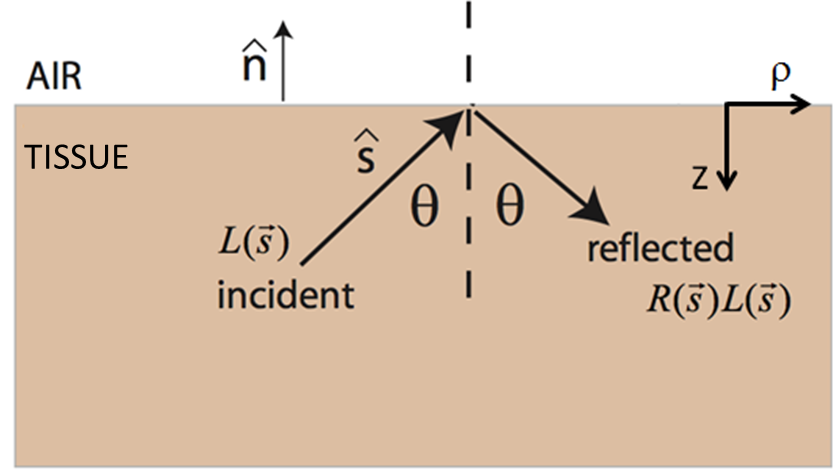
\includegraphics[width=8cm]{./figures/2_Theory/BoundaryReflect.png}
\caption[Diagram of air-tissue boundary]{At the air-tissue boundary, a fraction of the incident radiance $L(\hat{s})$ is Fresnel reflected ($R(\hat{s})$) back into the turbid medium due to index mismatch. This reflected light $R(\hat{s})L(\hat{s})$ accounts for all light diffusing inwards into the medium at the boundary. The boundary condition is derived using this observation. $\hat{n}$ is the unit vector normal to the air-tissue boundary. $z$ increases downward into the tissue and $\rho$ is parallel with the boundary.}
\end{figure}
The solution of this equation leads us to the well-known partial-flux boundary condition \cite{Haskell1994,Aronson1995}, i.e.,
\begin{align}
\Phi + \ell \nabla \Phi\cdot\mbf{\hat{n}} = 0 \label{eqn:BC_DE} \ ; \\ 
\ell = 2D\frac{1+R_{eff}}{1-R_{eff}} \ .
\label{eqn:extrap}
\end{align}
Here $R_{eff}$ is the effective reflection coefficient due to the index of refraction differences at the interface \cite{Orchard1969,Godavarty2002}. The positive parameter, $\ell$ (Equation~\ref{eqn:extrap}), is called the extrapolated boundary length; it corresponds to the distance (along the direction normal to the interface) for which the solution to Equation~\ref{eqn:BC_DE} is zero. (Note, this result is obtained with the Taylor expandsion of the fluence rate around its value at the interface, while keeping only the terms up to first order). Again, the details of this approach have been worked out in \cite{Haskell1994,Aronson1993,Aronson1995,Durduran2010}, and I will not carry out the derivation here. The resulting so-called extrapolated boundary condition is:
\begin{equation}
\Phi(z=-\ell)= 0 \ .
\end{equation}

We will use this extrapolated boundary condition to construct the Green's functions for semi-infinite and slab media. These Green's functions (or some equivalent form), in turn, facilitate solution of the problem when the turbid medium is heterogeneous. Of course, this latter situation is important for imaging inside a breast with cancerous lesions.
%
\subsection{Analytical Solutions}
This section covers three analytical solutions to the photon diffusion equation. We will solve for the fluence rate, $\Phi$, in homogenous turbid media in the infinite, the semi-infinite, and the slab geometries. For the infinite medium, we will derive the Green's function. For the semi-infinite and slab problems we will use the method of images and the extrapolated boundary condition to derive new Green's functions. 

\subsubsection{Infinite Geometry}
The simplest case we consider is the infinite geometry. Starting with the diffusion equation in the frequency domain (Equation~\ref{eqn:DE}), we assume that both the diffusion coefficient and the absorption coefficient of the medium are constant (i.e., the medium is homogeneous). Further, we assume that the point light source sits at the origin of the coordinate system. After dividing both sides by $D$, and defining the constant $k_0^2 = \frac{- v\mua^0 + i\omega}{D}$, (Equation ~\ref{eqn:DE}) can be written in the following Helmholtz-like form:
%
\begin{equation}
\label{eqn:DEhelm}
(\nabla^2+k_0^2)\Phi(\mbf{r},\mbf{r}_s)=-\frac{S}{D}\delta(\mbf{r}-\mbf{r}_s) \ .
\end{equation}
%
\noindent
Note, in this form, the photon fluence rate, $\Phi$, due to a point source is proportional to the Green's function solution (in this case the proportionality constant is $S/D$) for the Helmholtz equation (i.e., for the Helmholtz-like equation above with the unusual wave-vector). This equation for the Green's function with point source at $\mbf{r_s}$ is:
%
\begin{equation}
\label{eqn:Ghelm}
(\nabla^2+k_0^2)G(\mbf{r},\mbf{r}_s)=-\delta(\mbf{r}-\mbf{r}_s) \ .
\end{equation}
%
\noindent
With the boundary condition that the fluence rate goes to zero at infinity we obtain the well-known result:
%
\begin{equation}
\label{eqn:Ginf}
G(\mbf{r},\mbf{r}_s) = \frac{1}{4\pi}\frac{e^{ik_o|\mbf{r}-\mbf{r}_s|}}{|\mbf{r}-\mbf{r}_s|} \ .
\end{equation}
%
This Green's function solution is an overdamped spherical wave that vanishes at infinity. The wave-vector has real and imaginary parts that depend on the absorption coefficient, the reduced scattering coefficient, and the modulation frequency. The photon fluence rate solution is computed by spatial convolution of the Green's function and source distribution (which can originate at only a single point, but need not).
%
\subsubsection{Semi-infinite Geometry}
Now that we have the Green's function solution for infinite media, it is straight-forward to derive related solutions in the semi-infinite geometry. A key assumption from the partial-flux boundary condition facilitates the solution: the fluence rate is zero at the so-called extrapolated boundary (which is typically close to the real air-tissue boundary) \cite{Haskell1994,Aronson1993,Aronson1995}. Thus, if we know the source position, then we can use the method of images to construct our Green's function such that it vanishes at the extrapolated boundary. Recall that the extrapolated zero boundary is located a distance $\ell$ from the air-diffusive media interface ($z=0$) as shown in figure \ref{fig:semiinf}. 

The solution for the semi-infinite geometry can be readily determined using the well-known method of images. If a source exits some distance $\ell + z_s$ away from the extrapolated boundary (i.e., in the turbid medium), then we must place a sink the same distance on the opposite side of the boundary to insure that the net fluence rate at the extrapolated boundary position (i.e., between the real and image sources) is zero (see figure \ref{fig:semiinf}). This method-of-images approach yields the Green's function for the semi-infinite medium. The Green's function with the source and image source is
%
\begin{equation}
\label{semisoln}
G(\rho_s=0,z_s;\rho,z) = \frac{1}{4\pi} \left( \frac{exp[ikr_+]}{r_+} 
- \frac{exp[ikr_-]}{r_-} \right) \ ;
\end{equation}
%
\begin{eqnarray}
\label{ext_both}
r_{+} = & \sqrt{\rho^2+(z-z_{+})^2} \ ; \nonumber \\
r_{-} = & \sqrt{\rho^2+(z-z_{-})^2} \ .
\end{eqnarray}
%
\noindent
Here $z_+=z_s$ is the position of the source and $z_-=-2\ell-z_s$ is the position of our image source. Note, typically the source position due to a light fiber located at the air-tissue interface is set to be at a distance (into the diffuse medium) equal to the reciprocal of the reduced scattering coefficient and measured from the air-tissue interface at $z=0$.  Finally, as was the case for the infinite medium, the photon fluence rate solution is computed by spatial convolution of the Green's function and source distribution (which can originate at a only one point, but need not).
%
\begin{figure}[t]
\centering
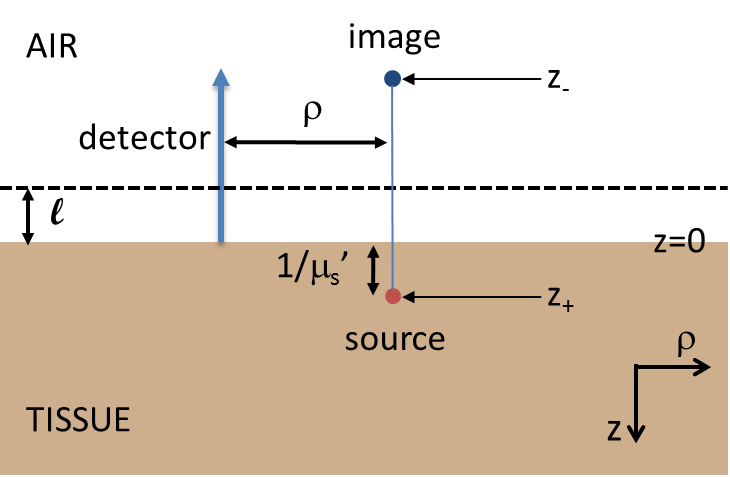
\includegraphics[width=8cm]{./figures/2_Theory/semiinf.png}
\caption[Diagram of the semi-infinite case]{The semi-infinite case where the method of images is used to find the solution of the Green's function. The $z$ direction increases downwards into the medium. $z_+$ is the location of the source, $z_-$ is the location of the image sink, and $z=0$ is the boundary between the tissue and air. The dotted line is where the extrapolated boundary is located a distance $\ell$ away from the boundary. $\rho$ is the distance between the source and detector fibers.}
\label{fig:semiinf}
\end{figure}
%
\subsubsection{Slab Geometry}
The solution for the slab geometry is just a more complicated variant of the solution for the semi-infinite case. We use the method of images again. This time, however, there is a second boundary, and we again make the assumption that $\Phi=0$ some distance $\ell$ away from the air/diffuse-media boundary for the second interface at $z=L$. As in the semi-infinite case, we add an image sink above the top ($z=0$) boundary, but now we also need to add another image sink below the bottom ($z=L$) boundary to the source.
\begin{figure}[h]
\begin{center}
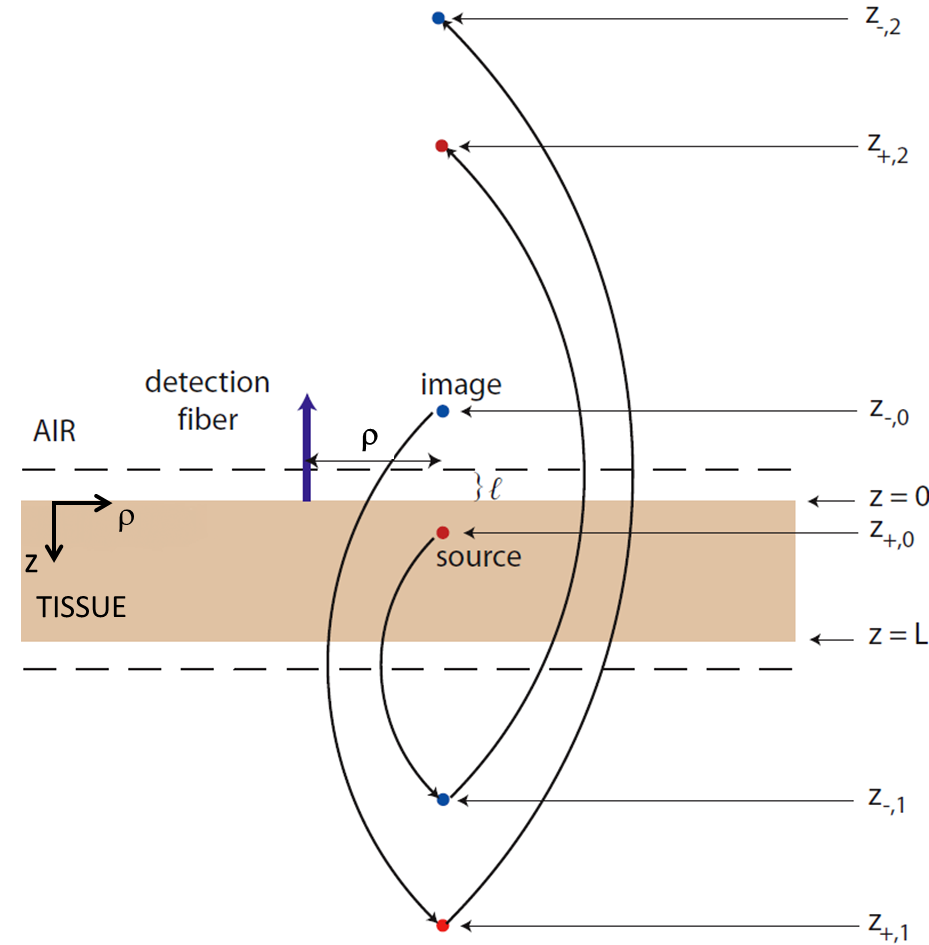
\includegraphics[width=10.5cm]{./figures/2_Theory/slab.png}
\caption[Diagram of the slab case]{The slab case where the method of images is used to find the solution of the Green's function. $z_+,0$ is the location of the source, $z_-,0$ is the location of the image sink, $z_+,1$ is the first source image, $z_-,1$ is the 2nd sink image and so on. $z=0,L$ is location of the boundaries between the tissue and air. The dotted line is where the extrapolated boundaries are located a distance $\ell$ away from the tissue/air boundaries. $\rho$ is the distance between the source and detector fibers. $z$ increases downwards into the slab.}
\label{fig:slab}
\end{center}
\end{figure}

Notably, every additional sink that is added would need its own image source, leading to a recursive procedure of adding sources and sinks. Therefore a pattern in the position of these sources and sinks emerge, and the Green's function for the original source and all the images can be written as an infinite sum:
\begin{equation}
G(\rho_s,z_s;\rho,z) = \frac{1}{4\pi} \sum_{m=-\infty}^{m=\infty} 
\left\{ \frac{exp[ikr_{+,m}]}{r_{+,m}} - \frac{exp[ikr_{-,m}]}{r_{-,m}} \right\} \ ;
\end{equation}
\vspace{-20mm}
\begin{eqnarray}
\label{ext_both}
r_{+,m} = & \sqrt{(\rho-\rho_s)^2+(z-z_{+,m})^2} \ ; \notag \\
r_{-,m} = & \sqrt{(\rho-\rho_s)^2+(z-z_{-,m})^2} \ .
\end{eqnarray}
\noindent
Here $z_{+,m}=2m(L+2\ell)+z_s$, $z_{-,m}=2m(L+2\ell)-2\ell-z_s$, $m=0,\pm 1, \pm 2, ...$, and $L$ is the thickness of the slab. For the semi-infinite geometry, only the $m=0$ term is used. 

Again, typically the source position due to a light fiber located at the air-tissue interface is set to be at a distance (into the diffuse medium) equal to the reciprocal of the reduced scattering coefficient; $z_{+,m}$ is positive as measured from air-tissue interface at $z=0$. Also, the terms in the sum are decreasing in size with distance of the image sources from the primary interface, so one typically does not have to keep too many terms to obtain good agreement between theory and experiment. Finally, as was the case for the infinite medium, the photon fluence rate solution is computed by spatial convolution of the Green's function and source distribution (which can originate at only one point, but need not).
%
\subsection{Multi-spectral Methods}
\subsubsection{Chromophore Absorption}
In tissues and other turbid media, the total absorption, $\mua$, is dependent on the relative concentrations of chromophores within the medium. If the number of chromophores is $N$, and they have spatial concentration distributions $c_i(\mbf{r})$,($i=1..N$), then 

\begin{equation}
\label{eqn:Chromo}
\mu_a(\lambda,\mbf{r}) = \sum_{i=1}^N c_i(\mbf{r}) \varepsilon_i(\lambda) \ .
\end{equation}
Here $\lambda$ is the wavelength of the probing light, and $\varepsilon_i$ is the wavelength-dependent extinction coefficient of chromophore $i$. The $\varepsilon_i$ are typically known from independent spectral measurements. Notice, it is possible to determine the chromophore concentrations, $c_i$, using this linear relationship. That is, the chromophore concentrations can be reconstructed directly from measurements of the absorption coefficient ($\mua$) at multiple wavelengths $\lambda_j$ ($j=1..M$), provided the number of independent equations ($M$) is equal to or greater than the number of unknowns ($N$). 

In breast tissue, the major chromophores are deoxy- (Hb), oxy-hemogloblin (${\rm HbO_2}$), lipid, and water (${\rm H_2O}$) in the near-infrared (NIR) wavelength range. The extinction coefficients for these chromophores are known \cite{Mourant1997,Doornbos1999,Wang2012,Jacques2013}. Furthermore, typical concentration values are known for breast, and this knowledge often helps to provide bounds/constraints on the allowed absorption in tomographic reconstructions. In our reconstructions in Chapter 4 the volume concentrations of water and lipid in the breast is assumed based on values from the literature \cite{Lee1997,White1987,Woodard1986}. 

Various analysis schemes are employed to extract physiological concentration information from the wavelength-dependent data. The traditional method determines an absorption coefficient at each wavelength, and then employs the equation above to extract chromophore concentrations. However, it is also possible to use all data at all wavelengths simultaneously to reconstruct chromophore concentrations. This latter, so-called multi-spectral approach has been shown to stabilize the reconstructions and to improve concentration fidelity \cite{Corlu2003,Srinivasan2005,Li2007}, provided that enough wavelengths are utilized.
%
\subsubsection{Scattering: Spectral Signatures from Mie Theory}
In tissue, the scattering properties are due to a number of factors, especially organelles (e.g., mitochondria, nuclei, cells, cell/tissue interfaces) and their concentration. In practice, the scattering coefficient, $\musp$, has been found to exhibit a power law variation as a function of wavelength in the NIR. Interestingly, this power law follows from a Mie scattering analysis too; the simplest Mie analysis assumes that all of the scattering is due to spherical particles of fixed size, but more complex analyses can add in particle size polydispersity, etc.

Mie scattering is a theory for light scattering from spherical particles based on Maxwell's equations. It is quite general, and it becomes especially important to use when the wavelength of the incident light becomes comparable to the particle size. 

Although Mie theory is old, its application to scattering in tissues in this context is relatively recent \cite{Mourant1997,Bevilacqua2000,Jacques2013}. If we assume a Mie scattering model as described above, then the wavelength dependence of the scattering coefficient,  $\musp$, has a power-law form: 
%
\begin{equation}
\musp(\lambda,\mbf{r}) = a(2\pi\varrho n_m)^b \lambda^{-b}  .
\end{equation}
%
Here $a$ is a constant that is proportional to the scatterer density, $\varrho$ is the radius of the spheres, $n_m$ is the index of refraction of the medium, and $b$ is the scattering power. In biomedical optics, this equation is often further simplified to
%
\begin{equation}
\label{eqn:Mie}
\musp(\lambda,\mbf{r}) = A(\mbf{r}) \lambda^{-b} \ .
\end{equation}
Here $A$ is called the scattering prefactor. A few papers have been published that fit scattering spectra from tissues, and, generally, $b$ is found to vary between 0.5 and 3 \cite{Bevilacqua2000,Jacques2013}. Notice, the spatial distribution of scattering model parameters, $A$ and $b$, can in principle be independently reconstructed from multi-spectral data \cite{Corlu2005}. However, it is quite common for experimenters to assume a fixed value for $b$ and then reconstruct $A$ and hence determine $\musp$. Since the NIR spectral range is not too broad, the scattering wavelength dependence is useful to employ in the reconstructions, which are often not very sensitive to the exact values of $A$ and $b$ in lieu of $\musp$.
%
\section{Reconstruction Methods}
The main rationale for using Diffuse Optical Tomography (DOT) in breast cancer imaging is that tumors have different physiological properties, such as vasculature, metabolic activity, organelle concenrations, and more, compared to surrounding healthy tissue. Furthermore, these differences in physiological properties are reflected as differences in optical properties, such as absorption and scattering coefficients.

Typical DOT instruments send photons into tissue at known points on the tissue surface (sources); output light that has traveled through the breast is then detected at known locations on the breast tissue surface (detectors). Importantly, this work is carried out in geometries that can be modeled reasonably with Green's function-based inverse problem approaches. Within these schemes, we utilize the measured data to solve for unknown $\mua$ and $\musp$ values in each volume element of the 3-dimensional image-space for the medium. Common reconstruction methods require two basic steps: 1) solving the forward problem and 2) solving the inverse problem (see Fig.~\ref{fig:forwardinverse}).

The forward problem, in essence, involves solving the diffusion equation for the fluence rate at known locations (e.g., within the medium or at the detector positions). The forward solution is readily determined, provided we are given specific values of $\mua$ and $\musp$ in each volume element within the sample, as well as information about input source locations and the tissue boundaries.

Solving the inverse problem is conceptually and technically more difficult than the forward problem. It involves determining new values of $\mua$ and $\musp$ from a comparison of the fluence rate at the boundary to the forward problem solution. Generally, as experimenters, we have knowledge about the diffuse light that we send into the medium and about the light that we measure after its emergence from the medium. The task of the inverse problem is to find unique solutions for the optical properties inside the medium, given this information.
%
\begin{figure}[t]
\centering
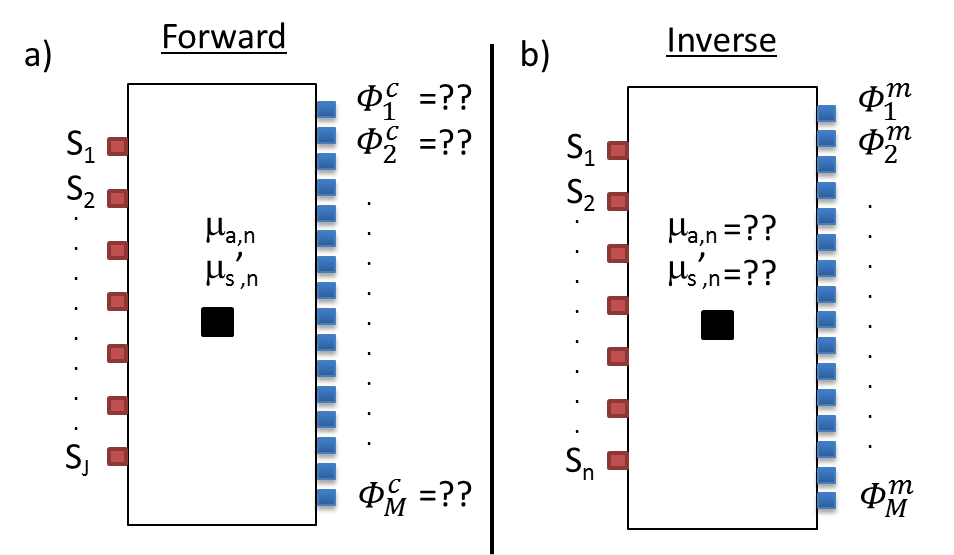
\includegraphics[width=10.5cm]{./figures/2_Theory/forwardinverse.png}
\caption[Forward and inverse problem diagrams]{a) Forward problem diagram (model) for slab geometry. The forward problem calculates the fluence $\Phi_{model}$ at detector locations, given values for the source ($S$) locations as well as $\mua$ and $\musp$ at $N$ voxel locations inside the turbid medium. b) Inverse problem diagram (experimental). From the measured value for the fluence at the boundaries $\Phi_{data}$, and the calculated fluence rate from the forward problem, the values for $\mua$, $\musp$ are updated/calculated.}
\label{fig:forwardinverse}
\end{figure}

For the forward problem, general theoretical approaches can be divided into three groups: Analytical methods, Numerical methods, and Monte-Carlo (MC) methods. These schemes range, respectively, from least to most computationally demanding. The analytical method is the fastest and easiest scheme (if we can figure out the analytic solution); given the source distribution, sample geometry, and optical properties, all that is required is a Green's function to generate the fluence rate within the medium (and on its boundaries). In principle, these analytical or semi-analytical approaches are well suited to use with very large data sets. However, the analytical approaches have limitations. These limitations come, in part, from “true” experimental geometries that differ from ideal cases and other experimental limitations such as small heterogeneities in the medium. Numerical methods, though more computationally intensive, are a bit more versatile. For example, by using numerical schemes, the number of assumptions about geometry are reduced, and it is possible to utilize well-worn techniques such as the Finite Element Method (FEM) and Finite Difference Method (FDM). The Monte-Carlo approach is a stochastic method which employs random step or Markov-chain models to account for transport of photons through the tissue; each of these photon trajectories is traced through the medium, with probability of absorption and scattering events included, until the photon exits or is absorbed. Though probably the most accurate method, this procedure employs a large number of photons ($>10^8$) and thus very computationally and time intensive. Of the methods described above, we will primarily investigate the first two groups.

The inverse problem is inherently more difficult than the forward problem; it involves the inversion of matrices (or similar/related mathematical operations). Such inversions are necessary to solve/update $\mua$ and $\musp$ from the measured and calculated fluence rates.  Standard inversions of the resulting sets of linear equations are non-trivial. For example, they can involve generating a pseudoinverse matrix (e.g., using singular value decomposition (SVD)). These operations are fast but are susceptible to large deviations due to the ill-conditioned matrices and noise, among other factors. A different approach to derive a solution is iterative and nonlinear (to varying degrees). In the nonlinear case, an iterative approach is utilized wherein the measured fluence is compared to the forward model (e.g., FEM model) solution of the diffusion equation using a cost function $\mbf{\Psi}$ (see Section \ref{sec:inverse}). The key iteration step chooses a direction in the solution-space and calculates (e.g., using either the Conjugate-Gradient (CG) method or the Gauss-Newton (GN) method) new optical property parameters; then the forward problem is solved again (with the new optical properties) and the iteration steps are repeated until a pre-set convergence criteria is reached. The nonlinear methods, while more accurate and flexible, are computationally very expensive and time consuming, especially when the data sets and the number of volume elements are large.

In the following sections we describe two inverse problem approaches using analytic (Section~\ref{sec:Analytic}) and algebraic (Section~\ref{sec:Algebraic}) linear schemes. Further, these reconstructions are used to analyze the experimental data described in Chapter 3. We will also discuss a nonlinear reconstruction method which is used for the experimental data in Chapter 4.
%
\subsection{Linear Reconstruction Methods}
\label{sec:linearrecon}
\subsubsection{Linearized Integral Equations}
\label{sec:rytov}
Here we derive linear solutions to the diffusion equation (\ref{eqn:DE}) in turbid media with heterogeneities. To simplify our problem, we divide the absorption and scattering (i.e., light diffusion coefficient) parameter into two parts: homogeneous background components and spatially heterogeneous (i.e., perturbative) components:
%
\begin{align}
\mua(\mbf{r}) &= \mua^0+\delta\mua(\mbf{r}) \ ; \\
D(\mbf{r}) &= D^0+\delta D(\mbf{r}) \ .
\end{align}

We use/substitute this perturbation expansion of the optical properties into the diffusion equation (Equation~\ref{eqn:DE}) in the presence of a single \textbf{point source} at $\mbf{r}_s$ (and we replace the fluence rate, $\Phi$, with the corresponding Green's function, $G$). Note, again, formally the fluence rate in this situation, $\Phi(\mbf{r}_s,\mbf{r})$, is proportional to the Green's function, $G(\mbf{r}_s,\mbf{r})$. Rearranging this resulting equation as described, we obtain:
%
\begin{equation}
\label{eqn:DEdiff}
\left[ - D^0 \nabla^2 + v\mu_a^0 - i\omega \right]G(\mbf{r}_s,\mbf{r})= \delta(\mbf{r}-\mbf{r}_s) - \Big[v\delta\mua(\mbf{r})-\nabla \cdot \delta D(\mbf{r})\nabla\Big] G(\mbf{r}_s,\mbf{r}) \ .
\end{equation}

The LHS of this equation is essentially the homogeneous diffusion equation with average/background values of absorption and diffusion. The spatially heterogeneous perturbations introduce important additional terms on the RHS of the equation. These terms account for how the fluence rate propagation is modified by the heterogeneous perturbations. We can manipulate this equation to derive an expression for the Green's function, $G(\mbf{r}_s,\mbf{r}_d)$, for a particular source-detector pair where $\mbf{r}_d$ is the detector position. The Green's function satisifes the Dyson equation:
\begin{equation}
\label{eqn:Dyson}
G(\mbf{r}_s,\mbf{r}_d) = G_0(\mbf{r}_s,\mbf{r}_d) - \int_V G_0(\mbf{r},\mbf{r}_d) [\delta\mu_a(\mbf{r}) - \nabla \cdot \delta D(\mbf{r}) \nabla] G(\mbf{r}_s,\mbf{r}) \ d^3 r \ .
\end{equation}
\noindent
Here the integral is taken over $V$, the full volume of our medium (i.e., the slab), and $G_0(\mbf{r}_s,\mbf{r}_d)$ is the analytic Green's function solution for the homogenous medium, i.e., homogenous slab, in this case.

This equation is intrinsically nonlinear, since $G(\mbf{r}_s,\mbf{r})$ depends on the optical properties too. Linearization involves the recursive substitution of the Green's function $G(\mbf{r}_s,\mbf{r})$ in the integrand, with Equation~\ref{eqn:Dyson}. The higher order terms are then neglected, leading to a linearized equation, where we have now excluded $G(\mbf{r}_s,\mbf{r})$ from the RHS. In addition, to simplify the notation, we let $\alpha(\mbf{r})=[v\delta\mu_a(\mbf{r}) - \nabla \cdot \delta D(\mbf{r}) \nabla]$. The lowest order linear solution, as might be expected from any Born expansion, is: 
\begin{align}
\label{eqn:LinDyson}
G(\mbf{r}_s,\mbf{r}_d) = G_0(\mbf{r}_s,\mbf{r}_d) - \int_V G_0(\mbf{r},\mbf{r}_d) \alpha(\mbf{r}) \
G_0(\mbf{r}_s,\mbf{r}) \ d^3 r \ .
\end{align}
\noindent
If, instead of the Born approximation the first Rytov approximation~\cite{Schotland1997} is adopted, Equation~(\ref{eqn:LinDyson}) yields: 
\begin{equation}
\label{eqn:linearDE}
G(\mbf{r}_{\rm d}, \mbf{r}_{\rm s}) = G_0(\mbf{r}_{\rm d}, \mbf{r}_{\rm s})
\exp\left[ -\int_V \frac{ G_0(\mbf{r}_{\rm d}, \mbf{r}) \alpha(\mbf{r})
G_0(\mbf{r}, \mbf{r}_{\rm s})\,d^3r}{G_0(\mbf{r}_{\rm d}, \mbf{r}_{\rm s})} \right] .
\end{equation}

Now let us connect this result to the data we might measure in an experiment. In practice, two independent measurements of the transmitted intensity are made. (Note, this intensity is derived from and is proportional to the diffuse light fluence rate at the output plane.) One measurement is made on a homogeneous (reference) media, and the another measurement is made on the medium with heterogeneities (i.e., the medium we want to understand). We denote these measurements by $I_0(\mbf{r}_{\rm d}, \mbf{r}_{\rm s})$ and $I(\mbf{r}_{\rm d}, \mbf{r}_{\rm s})$, respectively, where $\mbf{r}_{\rm d}$ and $\mbf{r}_{\rm s}$ are vectors specifying the positions of the detector and the source. Note, in my experimental work in Chapters 3 and 4, these quantities, $I_0$ and $I$, are ultimately derived from measured CCD counts in particular CCD pixels with specific integration times; the number of CCD counts in each pixel is linearly proportional to the corresponding photon fluence rate from the detected region. These measurements are readily connected to Green's function (which is also proportional to the fluence rate) and thus related to the optical properties of the sample medium through the relations:
\begin{align}
\label{eqn:Intensity1}
I(\mbf{r}_d, \mbf{r}_s) &= C_d(\mbf{r}_d)C_s(\mbf{r}_s)G(\mbf{r}_d,\mbf{r}_s) \ ; \\
\label{eqn:Intensity2}
I_0(\mbf{r}_d, \mbf{r}_s) &= C_d(\mbf{r}_d)C_s(\mbf{r}_s)G_0(\mbf{r}_d,\mbf{r}_s) \ .
\end{align}
\noindent

As noted above, $G(\mbf{r}_d,\mbf{r}_s)$ is the Green's function solution that is proportional to the fluence rate we should measure with our CCD. The quantities $C_d(\mbf{r}_d)$ and $C_s(\mbf{r}_s)$ are unknown coupling coefficients on the detectors and sources respectively. The coupling coefficients are cancelled out (in principle) when we normalize the true sample data by the reference measurement for the reconstructions (i.e., when we compute $I/I_0$).

We divide both sides of Equation~\ref{eqn:linearDE} by $G_0$, and take the natural log of both sides of the resulting equation. Finally we multiply both sides by $-G_0$ and obtain:
\begin{align}
-G_0(\mbf{r}_{\rm d}, \mbf{r}_{\rm s}) \ln\bigg[\frac{G(\mbf{r}_{\rm d}, \mbf{r}_{\rm s})}{G_0(\mbf{r}_{\rm d}, \mbf{r}_{\rm s})}\bigg] &= \int_V G_0(\mbf{r}_{\rm d}, \mbf{r}) \alpha(\mbf{r}) G_0(\mbf{r}, \mbf{r}_{\rm s})\,d^3r \ ; \\
\phi(\mbf{r}_d,\mbf{r}_s) &= \int_V G_0(\mbf{r}_{\rm d}, \mbf{r}) \alpha(\mbf{r}) G_0(\mbf{r}, \mbf{r}_{\rm s})\,d^3r \ .
\label{eqn:linearphi}
\end{align}
Here we define the so-called Rytov data function, $\phi(\mbf{r}_d,\mbf{r}_s)$ as
\begin{equation}
\label{eqn:datafunction}
\phi(\mbf{r}_d,\mbf{r}_s) =-G_0(\mbf{r}_{\rm d}, \mbf{r}_{\rm s}) \ln\bigg[\frac{I(\mbf{r}_{\rm d}, \mbf{r}_{\rm s})}{I_0(\mbf{r}_{\rm d}, \mbf{r}_{\rm s})}\bigg] \ .
\end{equation}
\noindent
Note, that the data function $\phi(\mbf{r}_d,\mbf{r}_s)$ is proportional to the measured fluence rate $\Phi(\mbf{r}_d,\mbf{r}_s)$. The right-hand side of the equation above contains the measured data function, and the left-hand side is an integral transform of the contrast within the sample. This formulation of the linearized DOT inverse problem is standard~\cite{Schotland1997}. 

\subsubsection{Analytical Inverse Reconstruction}
\label{sec:Analytic}
The analytical inverse reconstruction method that describe here and use in Chapter 3 was pioneered by my collaborators \cite{Markel2001,Markel2002,Markel2002a,Markel2003,Markel2003a,Markel2004,Konecky2008a}. Its application in the slab geometry has been reported in Refs.~\cite{Wang2005,Konecky2008a,Ban2013}. In this method, the inverse problem is simplified by taking advantage of symmetries which reduce the complexity of the Green's function while also enabling simplified data inversions through the use of the Fourier transform. To achieve this goal, one first decomposes the Green's function into plane waves so that it has the following form:
\begin{equation}
\label{eqn:Gplanes}                                               
G(\mbf{r},\mbf{r}^{\prime}) = \frac{1}{(2\pi)^3}\int d^3k \ g(k) \ e^{i\mbf{k} \cdot (\mbf{r}-\mbf{r}^{\prime})} \ .
\end{equation}
Here $g(k)$ gives the amplitude and phase for each plane wave. For complex boundaries, it is impossible to solve for $g(k)$. However, for some simple symmetric geometries (i.e., semi-infinite, slab, cylindrical, spherical), formulas for the Fourier components can be derived \cite{Markel2002a}.
\begin{figure}
\label{fig:slabcoord}
\centering{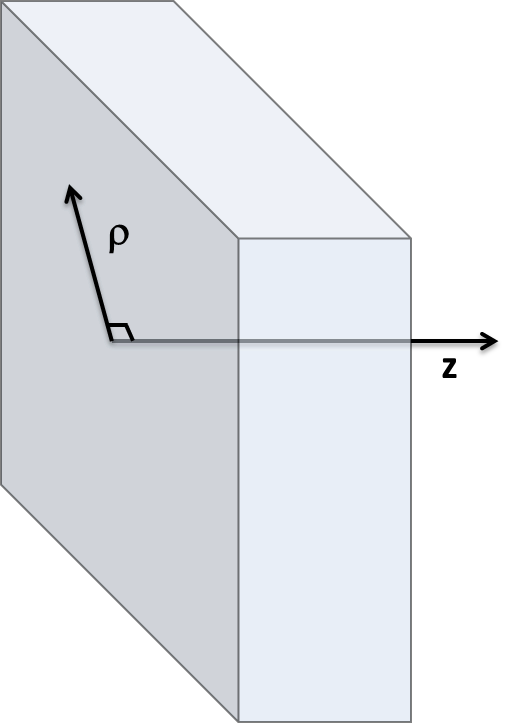
\includegraphics[width=5.5cm]{./figures/2_Theory/slabcoord.png}}
\caption[Slab geometry diagram]{Coordinates in the slab geometry. The positive z direction points into the slab while $\rho$ is parallel to the surface.}
\end{figure}

Our experiments in Chapters 3 and 4 are carried out in the slab geometry. Therefore, we will study the specifics of the slab geometry. In the slab, we define $\mbf{r} = (\mbf{\rho},z)$ where $z$ is depth in the medium and $\mbf{\rho}$ is parallel to the surfaces (see Fig.~\ref{fig:slabcoord}). In the Fourier space, $\mbf{k}=(\mbf{q},k_z)$. The form of the Helmholtz equation is thus modified: 
\begin{equation}
\label{eqn:slabhelm}
(\nabla^2_{{\bm \rho}} + \frac{\partial^2}{\partial z^2} + k_0^2)G(\mbf{r},\mbf{r}^{\prime}) = \frac{-1}{D_0} \delta (\mbf{r}-\mbf{r}^{\prime}) \ .
\end{equation}
Since no translational symmetry exists in the $z$ direction, we expand the Greens function in plane waves along ${\bm \rho}$. Then
\begin{equation}
\label{eqn:G_slab}
G(\mbf{r},\mbf{r'}) = \frac{1}{(2\pi)^2} \int d^2q \ g(q,z,z') e^{i\mbf{q} \cdot ({\bm \rho}-{\bm \rho}^{\prime})} \ .
\end{equation}
\label{eqn:g_1d}
Substitution of Equation~\ref{eqn:G_slab} into Equation~\ref{eqn:slabhelm} gives a one-dimensional differential equation for each value of $\mbf{q}$.
\begin{equation}
\left(\frac{\partial^2}{\partial z^2} - (q^2-k_0^2) \right) g(q,z,z') = \frac{-1}{D} \delta (z-z') \ .
\end{equation}
Although I will not write out the derivation here (see reference \cite{Konecky2008,Konecky2008a}), please note that g(q,z,z') can be solved for in the slab geometry and has the form:
\begin{equation}
\label{eqn:g_slab}
g(q;z,z') = \frac{\ell}{D} \frac{{\rm sinh}[Q(L-|z-z'|)]+Q\ell {\rm cosh}[Q(L-|z-z'|)]}{{\rm sinh}(QL)+2Q\ell {\rm cosh}(QL)+(Q\ell)^2{\rm sinh}(QL)}
\end{equation}
where $Q = q^2 -k_0^2$, $L$ is the slab thickness, and $\ell$ is the extrapolated boundary distance.

\subsubsection{Fourier Inversion Equations}
We next derive the inversion equations. We begin by substituting the plane wave Green's function (Equation~\ref{eqn:G_slab}) into the linearized forward equation we must solve (i.e., Equation~\ref{eqn:linearphi}). This substitution yields the following equation for the data function:
%
\begin{eqnarray}
\label{eqn:linearphiG}
\phi(\mbf{r}_s,\mbf{r}_d) = & \frac{1}{(2\pi)^4} \int d^2q_s \int d^2q_d \int d^3r \ g(q_d,z,z_d) {\rm exp}[i\mbf{q}_d \cdot ({\bm \rho} - {\bm \rho}_d)] \ ; \nonumber \\
 & \times \alpha(\mbf{r}) \ g(q_s,z_s,z) {\rm exp}[i\mbf{q}_s \cdot ({\bm \rho}_s - {\bm \rho})] \ .
\end{eqnarray}
%
For discrete source-detector pairs, the Fourier transform and the substitution of $\mbf{q} = \mbf{q}_s + \mbf{q}_d$, and $\mbf{p}=-\mbf{q}_s$, gives us a set of separate integral equations for each value of $q$:
%
\begin{equation}
\label{eqn:1Dfourier}
\tilde{\phi}(\mbf{q}_s, \mbf{q}_d) = \int_{z_s}^{z_d} \ \left[
\kappa_A(\mbf{q}_s,\mbf{q}_d;z)\ c \ \delta \tilde{\mu}_a(\mbf{q}_s+\mbf{q}_d) +
\kappa_D(\mbf{q}_s,\mbf{q}_d;z) \ \delta \tilde{D}(\mbf{q}_s+\mbf{q}_d) \right] dz
\end{equation}
%
where
\begin{align}
\label{kappaA}
\kappa_A(\mbf{q},\mbf{p};z) & = g(-\mbf{p};z_s,z) g(\mbf{q}+\mbf{p};z,z_d) \ ; \\
\label{kappaD}
\kappa_D(\mbf{q},\mbf{p};z) & = \frac{\partial g(-\mbf{p};z_s,z)}{\partial z}\frac{\partial g(\mbf{q}+\mbf{p};z,z_d)}{\partial z}+\mbf{p} \cdot (\mbf{q}+\mbf{p}) \ g(-\mbf{p};z_s,z) g(\mbf{q}+\mbf{p};z,z_d) \ .
\end{align}
%
Each integral in Equation~(\ref{eqn:1Dfourier}) can be inverted independently, thereby reducing computation time. From these results, we obtain inverse equations for $\mua$ and $D$ (and thus $\musp$).

Specifically:  1) we compute the Fourier transform of Equation~(\ref{eqn:linearphiG}) to obtain Equation~(\ref{eqn:1Dfourier}); 2) then we solve for $\delta \mua(\mbf{q},z)$ and $\delta D(\mbf{q},z)$ using singular value decomposition; 3) finally, the inverse Fourier transform for a given value of $z$ is computed with the equations below.
\begin{equation}
\delta \mu_a(\mbf{r}) = \frac{1}{(2\pi)^2} \int d^2q {\rm exp}(-i \mbf{q} \cdot {\bm \rho}) \sum_{\mbf{r},\mbf{p}} \kappa_A^*(\mbf{q},\mbf{r};z) \ [\kappa\kappa^*]^{-1}(\mbf{q},\mbf{r},\mbf{p}) \tilde{\phi}(\mbf{q},\mbf{p}) \ .
\end{equation}
\begin{equation}
\delta D(\mbf{r}) = \frac{1}{(2\pi)^2} \int d^2q {\rm exp}(-i \mbf{q} \cdot {\bm \rho}) \sum_{\mbf{r},\mbf{p}} \kappa_D^*(\mbf{q},\mbf{r};z) \ [\kappa\kappa^*]^{-1}(\mbf{q},\mbf{r},\mbf{p}) \tilde{\phi}(\mbf{q},\mbf{p}) \ .
\end{equation}
Here $\kappa_A^* [\kappa\kappa^*]^{-1}$ is the SVD pseudoinverse.

As an aside, note that the computational complexity of the analytical reconstruction is $O(N_q N_p^3)$, where $N_q$ is the number of discrete values of the vector $\mbf{q}$, and $N_p$ is the number of discrete values of $\mbf{p}$ in Equation~\ref{eqn:1Dfourier}. In the numerical implementation of the analytical method in Chapter 3, we have closely followed reference~\cite{Konecky2008a} and used a total of $49\times3249\simeq1.6\times10^5$ independent Fourier-space data points. Using these parameters, the necessary computations require $7\times 10^{9}$ floating point operations. On a single-core Intel Core 2 Duo processor with a peak performance of 19 GFlops, this calculation translates to 7 minutes of computation time.

\subsubsection{Algebraic Method}
\label{sec:Algebraic}
\label{subsec:alg_rec}
In general, variants of the algebraic image reconstruction are among the most popular methods per linear inversion techniques that have been applied to DOT \cite{Kak1987,OLeary1995,Ntziachristos2000,Intes2002}. These reconstructions are obtained by discretization of the volume integral in Equation~(\ref{eqn:linearphi}) and subsequent computation of the pseudo-inverse of the obtained system of linearized equations~\cite{Gonatas1995}.  This method does not require large windows (i.e., it does not need the large field-of-views which are required by symmetry in the analytic inversions), and it can be used with any type of data restriction. For the case of the analytical reconstruction method, on the other hand, for data restriction, it must be assumed that the data function $\phi=0$ (see Equation~(\ref{eqn:linearphi}) at these data points (i.e., $\Phi / \Phi_0=1$ at these restricted data points). On the other hand, the algebraic method requires explicit volume discretization in terms of voxels, while the analytical method allows one to reconstruct the target $z$ plane without much additional effort and is not dependent on volume discretization.

For the purpose of obtaining algebraic reconstructions we divide the slab into cubic voxels. In the discretization we approximate the integral in Equation~(\ref{eqn:linearphi}) with a Riemann sum, resulting in a system of algebraic equations $Ax=\phi$ where $A_{mn}$ is the $M\times N$ weight matrix, where $M$ is the number of distinct source-detector pairs, $N$ is the number of voxels, $x_n = \delta\alpha(\mbf{r}_n) / \alpha_0$ is the vector of dimensionless contrast $(n=1,\dots,N)$, and $\phi_m$ is the $m$-th data point $(m=1,\dots,M)$.  The equations are cast in dimensionless form by defining a dimensionless Green's functions according to $\tilde{G}_0(\mbf{r}, \mbf{r}^\prime) = D_0 h G_0(\mbf{r}, \mbf{r}^\prime)$, where $D_0$ is the diffusion coefficient in the background solution. Then we have:
%
\begin{align}
\label{eq6}
A_{mn} &= (k_{\rm d} h)^2 \tilde{G}_0(\mbf{r}_{{\rm d}m}, \mbf{r}_n) \tilde{G}_0(\mbf{r}_n, \mbf{r}_{{\rm s}m}) \ ; \\
\phi_m &= -\tilde{G}_0(\mbf{r}_{{\rm d}m}, \mbf{r}_{{\rm s}m}) \ln\left[\frac{I(\mbf{r}_{{\rm d}m}, \mbf{r}_{{\rm s}m})} {I_0(\mbf{r}_{{\rm d}m}, \mbf{r}_{{\rm s}m})}\right] .
\end{align}
%
\noindent
Here $k_d=\sqrt{\alpha_0/D_0}$, $\mbf{r}_n$ is the position of the center of the $n$-th voxel, and $\mbf{r}_{{\rm d}m}$, $\mbf{r}_{{\rm s}m}$ are the detector and source positions of the $m$-th data point used in the reconstruction.

The pseudoinverse solution to the above system of equations is defined as the unique solution to the system $(A^*A + \lambda^2 I)x = A^*\phi$, where $\lambda$ is the regularization parameter and $I$ is the identity matrix. In the experiments in Chapter 3, the number of measurements $M$ is much larger than the number of voxels $N$ (e.g., $M\sim 10^7$ and $N\sim 10^4$). Correspondingly, the most time consuming part of finding the pseudoinverse (at least, with the numerical approach we used) is the computation of the matrix product $A^*A$. In the most challenging case considered, we have used $M=2\times 10^7$ and $N=2\times 10^4$, which requires $8\times 10^{15}$ floating point operations. 

On an 8-core Xeon workstation with the peak performance of 56 GFlops, this calculation translates into 40 hours of computation time. However, this time-consuming procedure need only be repeated once for a given source-detector arrangement and given optical properties of the background medium; this situation is the case for my experiment in Chapter 3. Importantly, the resultant matrix, $A^*A$, once computed, can be stored on a hard drive and re-used for image reconstruction with each new data set obtained, e.g., for various positions of the chest wall phantom.  Furthermore, computation of the projection, that is, of the $N$-component vector $A^*\phi$, involves only one matrix-vector multiplication, and its computational cost is insignificant. In our case, the matrix $A^*A$ is small enough to be diagonalized; its eigenvectors and eigenvalues can be also stored on a hard drive for future use. In the reconstructions of Chapter 3, however, we solved the equation $(A^*A+\lambda^2I)x=A^*\phi$ directly by the conjugate-gradient descent method \cite{Hestenes1952}.

\subsection{Nonlinear Reconstruction Methods}
For the approaches described thus far, the tomography problem was linearized. Ultimately, however, it is desirable to employ nonlinear methods to find the solution, because in general the relationship between the measurements made and the unknown optical parameters is nonlinear. Among the advantages of the nonlinear reconstruction methods is that one typically has no restrictions on the experimental geometry; further, no linear assumptions are made to solve the diffusion equation, i.e., as we did in Section~\ref{sec:rytov}. While these conditions usually result in the problem being computationally intensive and time consuming, this drawback is typically compensated with parallelization of the problem. The nonlinear method we employ in this thesis is a model-based reconstruction technique. A forward model of light propagation generates an expected fluence rate, and then we seek to iteratively minimize the differences between our measurement and our model (forward) data by updating the parameters in the forward model. The forward model (diffusion equation) is solved using the finite element method (FEM).
%
\subsubsection{Finite Element Method}
\label{sec:FEM}
The FEM programs I employ are already standardized functions in most inversion software. Nevertheless, here I will quickly describe the basic premise of FEM for DOT, and I refer the interested reader to the literature for a more complete treatment \cite{Arridge1993,Paulsen1995}. To solve the forward problem with FEM, we first define a diffusion equation operator $\mathcal{L} =-\nabla \cdot D(\lambda)\nabla+\mua(\lambda)+i\omega/v$ such that: 
\begin{equation}
\label{eqn:DE_FEM}
\mathcal{L}\Phi(\mbf{r})=q_0(\mbf{r}) \ .
\end{equation}
Here $q_0(\mbf{r})$ is a our source term (note, it doesn't have to be a point source). The boundary condition used here is the Robin-type (partial flux) boundary condition: 
%
\begin{equation}
\Phi(r_b)+ \frac{D(z_b)}{\alpha}\mbf{\hat{n}}\cdot\nabla\Phi(r_b)=0 \ .
\end{equation}
Here $r_b$ is a point on the measurement boundary and $\alpha$ is a refractive index mismatch term \cite{Arridge2000}. Assuming that our detected signal is the normal component of the photon flux $\phi_m = \mbf{\hat{n}}\cdot[-D(r_b)\nabla\Phi(r_b)]$, the equation in the case of the Robin boundary condition simplifies to
\begin{equation}
\phi_m(r_b)=\alpha\Phi(r_b) \ .
\end{equation}

The volume $\Omega$ we are interested in imaging (in our case the slab) is discretized into $V$ vertex nodes. If $ u_i(\mbf{r})$ is a basis function from a V-dimensional subspace, then the approximate piecewise continuous polynomial FEM solution to $\Phi(\mbf{r})$ is 
\begin{align}
\Phi^h(\mbf{r})= \sum_i^V \Phi_i u_i(\mbf{r}) \ .
\end{align}
\noindent
The linear or higher order basis functions are defined over triangle (2D), tetrahedral (3D), or square grid elements (3D, used in TOAST++ \cite{Schweiger2014}).

To find the appropriate basis vectors $u_i(\mbf{r})$, we minimize the residual defined as:
\begin{align}
\label{eqn:FEM_R}
\mathcal{L}\Phi(\mbf{r}) - q_0(\mbf{r})
&= R, \\
&= \sum_i^V R_i u_i(\mbf{r}) \ ,
\end{align}
%
by requiring that $R$ be orthogonal to $u_i$ (for $i=1...V$) which in Equation~\ref{eqn:FEM_R} gives
\begin{equation}
\label{eqn:FEM}
(\mbf{K}(D) + \mbf{C}(\mua) + i\omega\mbf{B} + \alpha\mbf{A})\mbf{\Phi}= \mbf{Q} \ ;
\end{equation}
\begin{align}
K_{ij} &= \int_\omega D(r)\nabla u_i(\mbf{r})\cdot\nabla u_j(\mbf{r}) d\Omega \ ; \\
C_{ij} &= \int_\omega \mua(r) u_i(\mbf{r})u_j(\mbf{r}) d\Omega \ ; \\
B_{ij} &= \frac{1}{v}\int_\omega u_i(\mbf{r})u_j(\mbf{r}) d\Omega \ ; \\
A_{ij} &= \int_{\dell\omega} u_i(\mbf{r})u_j(\mbf{r}) d(\dell\Omega) \ ;
\end{align}
\begin{equation}
q_{0,i} = \int_{\omega} \mua(r) u_i(\mbf{r})q_0(\mbf{r}) d\dell\Omega \ .
\end{equation}
Here $\mbf{\Phi}$ is the FEM basis expansion coefficient vectors for $\Phi(\mbf{r})$. These equations are the FEM discretization of the diffusion equation. Note that $\mbf{K},\mbf{C},\mbf{B},$ and $\mbf{A}$ are matrices of size $V\times V$. Equation~(\ref{eqn:FEM}) can can be inverted to give us our forward solver using Cholesky factorization (CW only), LU Decomposition, or iterative solvers like the Conjugate-Gradient method and GMRES.

\subsubsection{The Inverse Problem}
\label{sec:inverse}
The central problem to image reconstruction lies in finding a solution vector $\mbf{\hat{x}}$ that best fits the measurement data where
\begin{equation}
\mathbf{x}=[\mua_{,1},\cdots,\mu_{,V},\musp_{,1}, \cdots, \musp_{,V}]^T \ .
\end{equation}
The elements of $\mathbf{x}$ are $\mua$ and $\musp$ (at a single wavelength) for every vertex of the volume that we want to reconstruct. A straightforward way to utilize multi-spectral data is to reconstruct $\mbf{x}$ for each wavelength, and then convert $\mua$ and $\musp$ to $C_i$ (where $i$ indexes the chromophore) and $A$ using the relationship given by Equation~(\ref{eqn:Chromo}) and (\ref{eqn:Mie}). (Note, the exponent $b$ can also be a free parameter if desired but is often fixed). It has been learned that multi-spectral methods stabilize various inverse problems \cite{Corlu2005,Corlu2003}, so the preferred method (when the data quality is good for many wavelengths) is to reconstruct for $C_i$ and $A$ utilizing all the data simultaneously in the inversion. Then $\mbf{x}$ is instead
\begin{equation}
\mathbf{x}=[C_{1,1},\cdots,C_{1,V}, \cdots, C_{K,1},\cdots, C_{K,V}, A_1, \cdots, A_V]^T
\end{equation}
\noindent
where the number of elements in $\mbf{x}$ is $N=[(K+1)\times V]$.

Finding the solution vector $\mbf{\hat{x}}$ can be approached as an optimization problem \cite{Arridge1998,Schweiger2005} wherein the solution $\mathbf{\hat{x}}$ is found by minimizing an objective function
%
\begin{equation}
\mbf{\hat{x}} = \arg \min_{\mbf{x}} \Psi(\mbf{x}) \ ,
\end{equation}
\noindent
where above we search for some parameter \mbf{x} that returns the minimum of $\Psi(x)$. Here $\Psi$ is defined
%
\begin{equation}
\label{eqn:Psi}
\Psi = \frac{1}{2}\sum_{l=1}^L\sum_{s=1}^S\sum_{d=1}^{D_s}\Big[\Phi^c(\mbf{x})-\Phi^m\Big]^2 \ .
\end{equation}
\noindent
The summations are over all source-detector pairs and wavelengths in the data sets, where $L$ is the number of wavelengths, $S$ is the number of source positions, and $D_s$ is the number of detector positions for a given source. The total number of measurements is $\ M=L\times(\sum_{s=1}^S D_s)\ $. $\Phi^c(\mbf{x})$ is the fluence rate calculated by our forward FEM (Section~\ref{sec:FEM}) and $\Phi$ is our measured fluence rate for a given source-detector pair, and thus the term to minimize is $[\Phi^c(\mbf{x})-\Phi]^2$.
%
\begin{figure}[h]
\centering
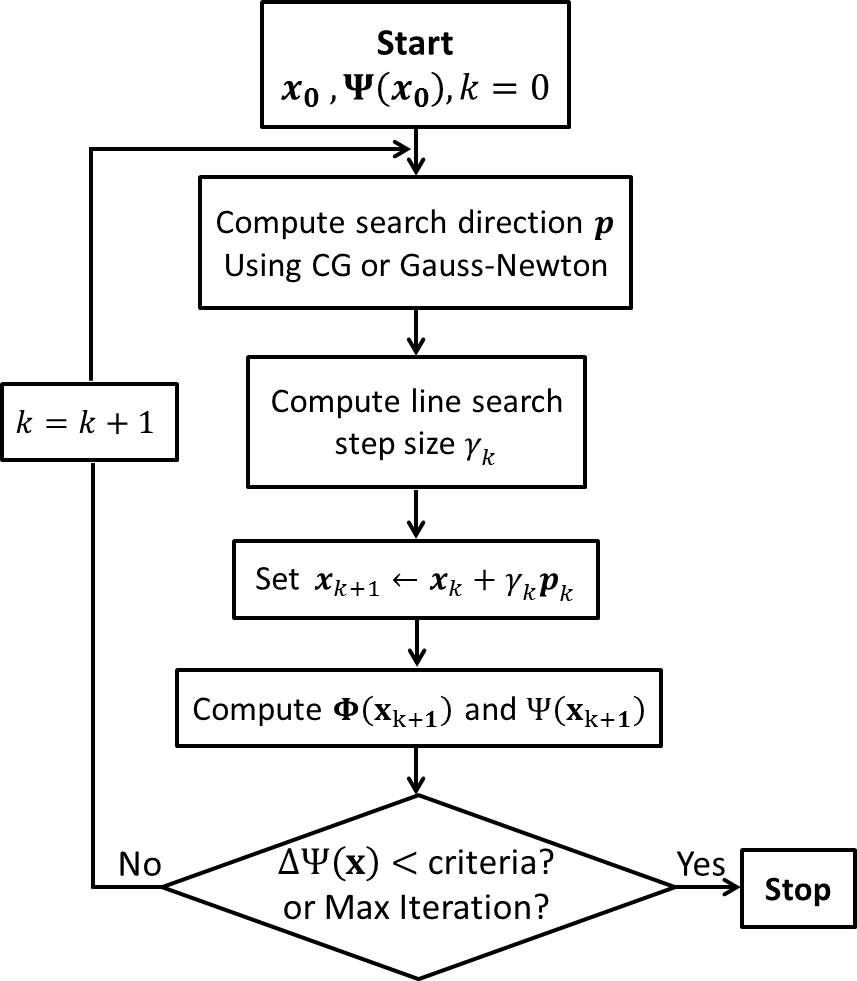
\includegraphics[width=9cm]{./figures/2_Theory/reconflow.png}
\caption{Reconstruction flowchart.}
\label{fig:reconflow}
\end{figure}
%
Fig.~\ref{fig:reconflow} is the flowchart for the image reconstruction algorithms. We start with an initial guess $\mbf{x_0}$ for the parameters, and then calculate the $\Psi$ function by solving the forward problem for $\mbf{\Phi^c(x)}$ and using the measured data $\mbf{\Phi^m}$. The parameter vector $\mbf{x_0}$ is updated by adding a scaled vector $\Delta \mbf{x} = \gamma_k\mbf{p_k}$. Then $\Psi$ is recalculated with the updated parameter vector and checked again to determine if the stopping criteria, which is set by the user to test how close the model fluence rate is to the data, is satisfied. If the criteria, or some maximum iteration number, is not met, then $x$ is updated again, and the loop is continued.

$\Delta\mbf{x}$ depends on the step size $\gamma$ and the step direction $\mbf{p}$. $\gamma$ is determined by a line search along $\mbf{p_k}$ that sufficiently minimizes $\Psi$:
\begin{equation}
\min_{\gamma}\mbf{\Psi(x}_k+\gamma\mbf{p_k}).
\end{equation}
The Taylor's expansion of our updated objective function $\mbf{\Psi(x}_k+\gamma\mbf{p}_k})$ is:
\begin{equation}
\label{eqn:PsiTaylor}
\mbf{\Psi(x}_k+\gamma\mbf{p}_k}) = \mbf{\Psi(x})_k+\gamma\mbf{p}_k^T\nabla\mbf{\Psi(x}_k) + \frac{1}{2}\gamma^2 \mbf{p}_k^T\nabla^2\mbf{\Psi(x})_k\mbf{p}_k + \cdots
\end{equation}
%
The search direction $\mbf{p}_k$ can be derived using either the first order derivative (Conjugate Gradient) or the second order derivative (Gauss-Newton). We will briefly discuss these methods in the following sections.
%
\subsubsection{Conjugate Gradient Method}
The Conjugate-Gradient technique is a commonly implemented method in DOT reconstruction algorithms. For a detailed derivation of the Conjugate Gradient (CG) method, I refer the reader to \cite{Arridge1998,Shewchuk1994}. Very briefly, to use the CG method, $\nabla\mbf{\Psi}$ from the 2nd term of Equation~(\ref{eqn:PsiTaylor}) is needed. It is
\begin{align}
\nabla\mbf{\Psi(x)} &= \mbf{J(x)^T F(x)} \label{eqn:dPsi} \ ; \\
f_i(\mbf{x}) & =\Phi^c_i(\mbf{x})-\Phi^m_i \ ; \\
\mbf{F(x)} &= \Big[f_1(\mbf{x}),f_2(\mbf{x}),\cdots,f_{M}(\mbf{x})\Big]^T \ .
\end{align}
where the Jacobian is
\begin{equation}
J=
\begin{bmatrix}
    \frac{\partial f_1(\mbf{x})}{\partial x_1} & \frac{\partial f_1(\mbf{x})}{\partial x_2} & \cdots & \frac{\partial f_1(\mbf{x})}{\partial x_N} \\
    \frac{\partial f_2(\mbf{x})}{\partial x_1} & \frac{\partial f_2(\mbf{x})}{\partial x_2} & \dots  & \frac{\partial f_2(\mbf{x})}{\partial x_N} \\
    \vdots & \vdots & \ddots & \vdots \\
   \frac{\partial f_M(\mbf{x})}{\partial x_1} & \frac{\partial f_M(\mbf{x})}{\partial x_2} & \dots  & \frac{\partial f_M(\mbf{x})}{\partial x_N}
\end{bmatrix} \ .
\end{equation}

For real experimental data in Chapter 4, the Jacobians are arranged as shown in Fig.~\ref{fig:jacobill}. The Jacobian is typically calculated for known $\mua$ and $\musp$. The image reconstruction software that we use (Toast++) readily provides the gradients for the standard DOT optical coefficients, i.e., 
\begin{equation}
f'^{(\mu_a)} = \frac{\partial \Phi}{\partial \mu_a}, \quad f'^{(\mu_s)} = \frac{\partial \Phi}{\partial \mu_s} \ .
\end{equation}
For multi-spectral data, we want the Jacobian to be written in terms of the chromophore concentration and the scattering factor and power A, b. The required gradients with respect to these parameters can be obtained by applying the chain rule:
\begin{eqnarray}
f'^{(c_i)} &=& \sum_{j=1}^L f'^{(\mu_a)}(\lambda_j) \frac{\partial \mu_a(\lambda_j)}{\partial c_i} = \sum_{j=1}^L f'^{(\mu_a)}(\lambda_j) \varepsilon_i(\lambda_j) \ ; \\
f'^{(A)} &=& \sum_{j=1}^L f'^{(\mu_s)}(\lambda_j) \frac{\partial \mu_s(\lambda_j)}{\partial A} = \sum_{j=1}^L f'^{(\mu_s)}(\lambda_j) \lambda_j^{-b} \ ; \\
f'^{(b)} &=& \sum_{j=1}^L f'^{(\mu_s)}(\lambda_j) \frac{\partial \mu_s(\lambda_j)}{\partial b} = \sum_{j=1}^L f'^{(\mu_s)}(\lambda_j) A \lambda_j^{-b} \ln{\lambda_j} \ .
\end{eqnarray}
%
Now we are able to use the Conjugate Gradient algorithm:
\begin{enumerate}[noitemsep]
\item Initialize: $k=0$
\vspace{-17mm}
\begin{align}
\mbf{r}_0 &=-\nabla\mbf{\Psi(x}_0) \ ; \\
\mbf{p}_0 &= \mbf{r}_0 \ .
\end{align}
\item Find step size (find $\gamma$):
\vspace{-10mm}
\begin{equation}
\min_{\gamma}\mbf{\Psi(x}_k+\gamma_k\mbf{p_k}) \ .
\end{equation}
\item Update parameters:
\vspace{-10mm}
\begin{equation}
\mbf{x}_{k+1} = \mbf{x}_{k} + \gamma_k \mbf{p}_{k} \ .
\end{equation}
\item Check \Big[$\mbf{\Psi(x}_{k+1})<$ criteria?\Big]: ~~~~~~\textbf{Yes:} Stop ~~~~~~\textbf{No:} Continue
\vspace{4mm}
\item Update direction vector:
\vspace{-17mm}
\begin{align}
\mbf{r}_{k+1} &=-\nabla\mbf{\Psi(r}_{k+1}) \ ; \\
\beta_{k+1} &= \frac{\mbf{r}^T_{k+1}(\mbf{r}_{k+1}-\mbf{r}_{k})}{\mbf{r}^T_{k}\mbf{r}_{k}} \ ; \\
\mbf{p}_{k+1} &= \mbf{r}_{k+1} + \beta_{k+1}\mbf{p}_{k} .
\end{align}
\item \vspace{-5mm} $k=k+1$. Move to Step 2.
\end{enumerate}
\begin{figure}[h]
\centering
\label{fig:jacobill}
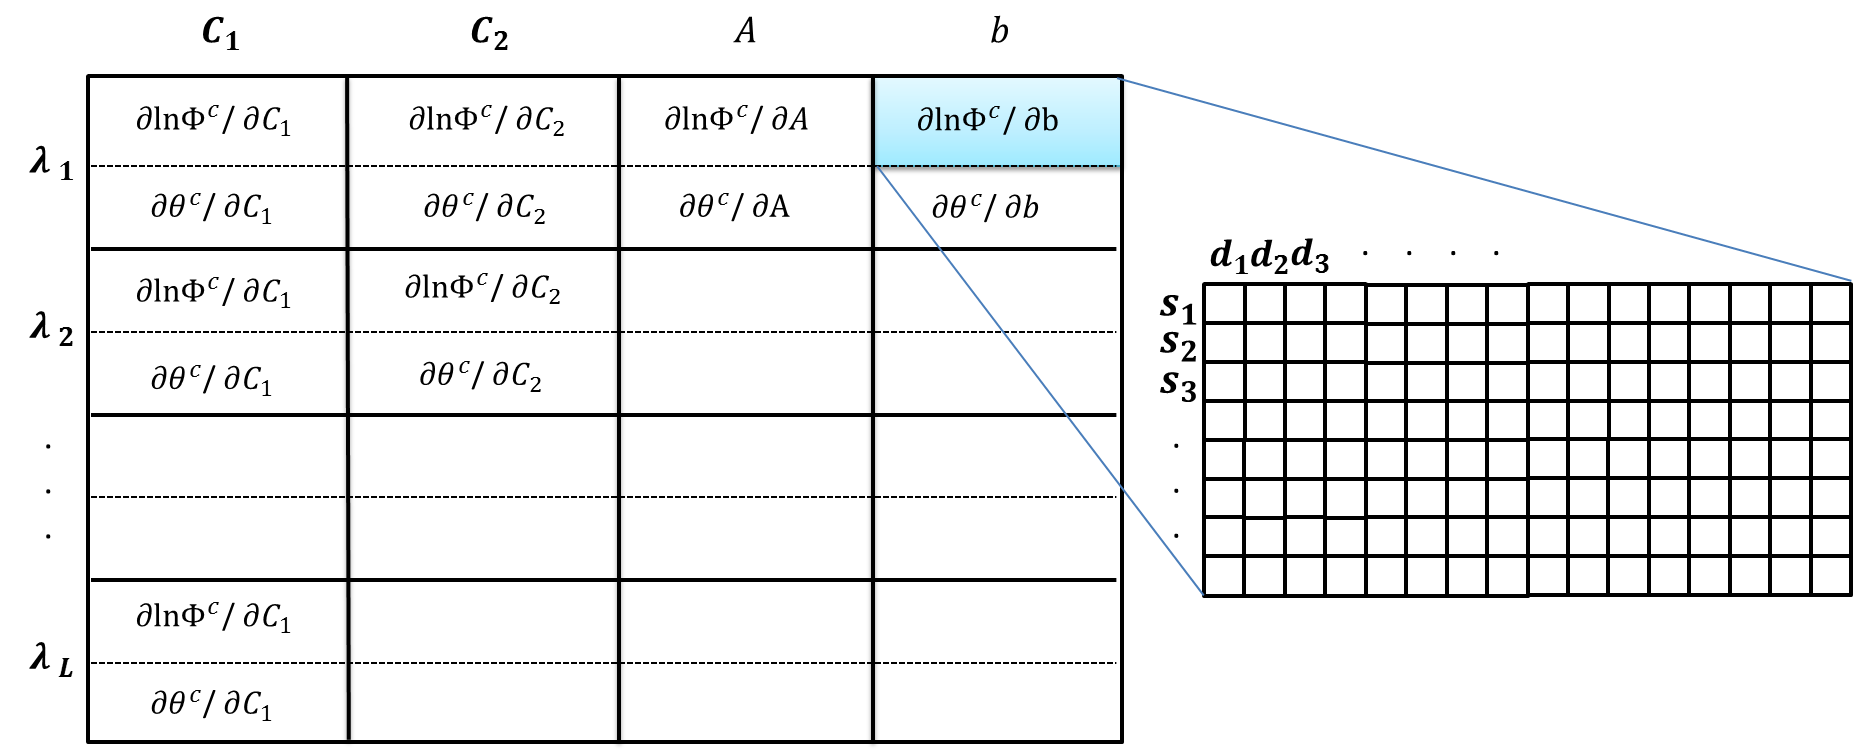
\includegraphics[width=14.5cm]{./figures/2_Theory/jacobschem.png}
\caption[Illustration of the Jacobian matrix for Gen3 imager datasets]{Illustration of the Jacobian matrix for datasets collected in Chapter 4. Row blocks are organized by wavelengths; they are further divided into amplitude and phase. Column blocks are organized by the chromophores ($C$), and A,b. The amplitude and phase data blocks (light blue) consist of data for every source-detector pair: the rows indexes the sources $s$ and the columns indexes the detectors $d$ for each source. }
\end{figure}
%
\subsubsection{Gauss-Newton Method}
The Gauss-Newton method is an iterative method that uses an approximation of second order derivatives in the cost function. Consider Equation~(\ref{eqn:PsiTaylor}) with $\gamma=1$. Let us assume that $\mbf{\Psi(x}_k+\gamma\mbf{p}_k})$ is twice differentiable. Beginning with Equation~(\ref{eqn:PsiTaylor}) and differentiating both sides with respect to $\mbf{p}_k$ we have:
%
\begin{equation}
\nabla\mbf{\Psi(x}_k+\gamma\mbf{p}_k}) = \nabla\mbf{\Psi(x}_k) + \nabla^2\mbf{\Psi(x})_k\mbf{p}_k \ .
\end{equation}
%
$\mbf{\Psi(x}_k+\gamma\mbf{p}_k})$ is minimized when $\nabla\mbf{\Psi(x}_k+\gamma\mbf{p}_k})=0$. The above equation then becomes:
%
\begin{equation}
\nabla^2\mbf{\Psi(x})_k\mbf{p}^{GN}_k = -\nabla\mbf{\Psi(x}_k) \ ,
\end{equation}
\noindent
where $\mbf{p}^{GN}_k$ is a vector that points in the Newton direction. We know $\Big[\nabla\mbf{\Psi(x}_k) = \mbf{2J(x}_k)^T \mbf{F(x}_k)\Big]$ from Equation~(\ref{eqn:dPsi}). $\nabla^2\mbf{\Psi(x})$ is
%
\begin{equation}
\nabla^2\mbf{\Psi(x}_k)=\sum_{m=1}^M\nabla^2(\mbf{\Psi(x}_k)^2)=\sum_{m=1}^M\mbf{H^m(x}_k) \ ,
\end{equation}
where $\mbf{H}^m(\mbf{x}_k)$ is the Hessian. Written out explicitly:
\begin{equation}
\nabla^2\mbf{\Psi(x}_k)= 2\mbf{J(x}_k)^T\mbf{J(x}_k)+\sum_{m=1}^M\sum_{i=1}^N\sum_{j=1}^N f_i(\mbf{x})\frac{\partial f_m(\mbf{x})}{\partial x_i \partial x_j} \ .
\end{equation}
\noindent
The second term is much smaller than the first term, and in the Gauss-Newton method an approximation is made wherein the second term is ignored such that:
%
\begin{equation}
\nabla^2\mbf{\Psi(x}_k)=2\mbf{J(x}_k)^T\mbf{J(x}_k) \ .
\end{equation}
%
Thus the main equation in the Gauss-Newton method is:
%
\begin{equation}
\label{eqn:GN}
2\mbf{J(x}_k)^T\mbf{J(x})_k\mbf{p}_k^N = -\mbf{2J(x}_k)^T \mbf{F(x}_k) \ .
\end{equation}

With this method to ascertain the Gauss-Newton direction $\mbf{p}_k^N$, this relation can be used repeatedly in an iterative manner. A line search method can also be added into the algorithm where the minimum is searched for along $\mbf{p}_k^N$. The Gauss-Newton algorithm is as follows:
\begin{enumerate}[noitemsep]
\item Initialize: k = 0
\item Evaluate:
\vspace{-17mm}
\begin{align}
\nabla\mbf{\Psi(x}_k) &= \mbf{2J(x}_k)^T \mbf{F(x}_k) \ ;\\
\nabla^2\mbf{\Psi(x}_k)&=2\mbf{J(x}_k)^T\mbf{J(x})_k \ .
\end{align}
\item Solve for $\mbf{p}_k^N$ in 
\vspace{-17mm}
\begin{align}
2\mbf{J(x}_k)^T\mbf{J(x})_k\mbf{p}_k^N &= -\mbf{2J(x}_k)^T \mbf{F(x}_k) \\
&{\rm(using~GMRES,~CG,~etc.)} \ . \notag
\end{align}
\item Compute $\gamma_k$ (line search) \ .
\item Update parameter:
\vspace{-10mm}
\begin{equation}
\mbf{x}_{k+1} = \mbf{x}_{k} + \gamma_i \mbf{p}_{k} \ .
\end{equation}
\item Check \Big[$\mbf{\Psi(x}_k)<$ criteria?\Big]: ~~~~~~\textbf{Yes:} Stop ~~~~~~\textbf{No:} Continue
\vspace{4mm}
\item Update $k=k+1$, go to Step 2.
\end{align}
\subsubsection{Levenberg-Marquardt Method}
The Levenberg-Marquardt Method is another technique commonly used in DOT reconstruction packages (e.g., TOAST++, NIRFAST) that I will very briefly summarize. The Levenberg-Marquardt Method is a variation on the Gauss-Newton method wherein a term is added to the Hessian in Equation~\ref{eqn:GN}
\begin{align}
2[\mbf{J(x}_k)^T\mbf{J(x})_k+\lambda I]\mbf{p}_k &= -\mbf{2J(x}_k)^T \mbf{F(x}_k)\ ; \label{eqn:LM-2}\\
\mbf{p}_k &= -2[\mbf{J(x}_k)^T\mbf{J(x})_k]^{-1}\mbf{2J(x}_k)^T \mbf{F(x}_k) \label{eqn:LM-2}\ .
\end{align}
$\lambda$ is called the damping parameter. This additional term has two main effects. The first effect is to increase the the number on the diagonals and therefore suppress the 2nd derivatives. A large $\lambda$ will result in the left hand side of the equation being more like the identity matrix, resulting in the steps becoming more like the steepest descent method. One common technique is to start with a large $\lambda$ and then decrease its value at each iteration (i.e., by half every iteration); this procedure causes a gradual switch from the gradient descent method to Gauss-Newton over each step of the reconstruction. The second effect that this additional term introduces is to limit the step size. Since they are inversely related with the search direction vector $\mbf{p}_k$ (Equation \ref{eqn:LM-2}), higher damping terms have the effect of decreasing the step size. This decrease in step size prevents large changes in the iteration at early steps which is useful when there could be instabilities due to errors in the initial guess. Overall these two functions have an effect of stabilizing the reconstruction in the early iterations.

\subsubsection{Regularization}
\label{sec:reg}
The image reconstruction problems we discussed above are generally ill-posed  and often under-determined (i.e., the number of independent measurements are less than the number of unknowns). Among the characteristics of ill-posed problems is that small changes in detected signals can induce large changes in the reconstructed optical properties This situation implies that the reconstructions have non-uniqueness problems and will require additional constraints to help achieve convergence. In practice the solution space is constrained or \textit{regularized} to utilize \textit{apriori} information. Generally, any scientist working on ill-posed image reconstruction (or ill-posed inverse problems) will utilize some type of regularization technique to optimize their images. In the medical imaging field, regularization is common.

For our nonlinear methods, regularization is typically introduced as a term in the objective function as shown below:
\begin{equation}
\Psi = \frac{1}{2}\sum_{l=1}^L\sum_{s=1}^S\sum_{d=1}^{D_s}\Big[\Phi^c(\mbf{x})-\Phi\Big]^2 + \Lambda R(\mbf{x})\ .
\end{equation}
\noindent
Here $\Lambda$ is the scaling factor, and $R(\mbf{x})$ is called the regularization functional. As in Equation~\ref{eqn:Psi}, $L$ is the total number of wavelengths, $S$ is the total number of sources, and $D_s$ is the number of detectors for a particular source $s$. The additional term can be thought of as a penalty on the cost function based on the regularization functional. A few examples are: $R=||\mbf{x-x_0}||^2_2$,  $R=||\nabla\mbf{x}||_1$, and $R=-\nabla\cdot(\nabla \mbf{x}/|\nabla\mbf{x}|)$; in these cases, the reconstruction is effectively penalized for large optical property excursions within the image based on, respectively, its difference, its gradient, or a function of its change in gradient. The relative importance of these  penalties is adjusted through the scaling factor $\Lambda$, which can be modified with each iteration as well. These kinds of regularization terms are useful when spatial information about the optical properties of the medium are known, or when some information about the optical property variations are expected. The more information one has in advance, the more that can be included in the cost function.

Throughout this thesis, I have explored the utility of various regularization schemes, and I have tried to identify the best ones for our problem. These tasks are non-trivial and have only just begun. In our reconstructions in Chapter 4, we found that the Total Variation (TV) method, which is an edge-preserving regularization, can work well. TV was applied to preserve contrast and to preserve transverse size of targets in our DOT reconstructions, but it also had the cost of increasing certain classes of artifacts. The particular form we used is $\Lambda\sqrt{|\nabla\mbf{x}|^2+\beta^2}$, which is actually an approximation of the TV method. Here $\beta>0$ is a small parameter added to deal with the non-differentiability of the absolute value $|\nabla\mbf{x}|$ when $\nabla\mbf{x}=0$. It is worth noting that it is also possible to employ different regularization multiplicative scaling terms for different optical parameters. For example, in our reconstructions in Chapter 4, we found that using a separate regularization factor for absorption and for scattering improved the spatial fidelity of the target reconstructions (see Section~\ref{sec:2Dsim} in Chapter 4).


\chapter{Imaging Breast Cancer: Chest Wall Effects}
\label{Chap:3_chestwall}
\vspace{-5mm}
\section{Introduction}
\vspace{-5mm}
Although various forms of diffuse optical tomography (DOT) have been employed to derive spatial maps of physiological features in the human breast with some success, the fidelity of these images is compromised by boundary effects such as those that arise from data obtained near the subject's chest wall. 

The breast is sometimes approximated as a slab, which allows the formulation of imaging problem with analytical Green's functions. The chest wall falls within the vicinity of the breast through which light can travel. Furthermore, from a general diffuse optics viewpoint, the very existence of the chest wall breaks the natural symmetry of the slab geometry, a symmetry which is often utilized when formulating Green's functions for the imaging problem. The chest wall introduces perturbations into the inverse problem that become more important as the source and detector locations move away from the nipple region and closer to the chest.

The DOT community has not dealt systematically with the influence of the chest wall. Dealing with these chest wall issues is the primary purpose of the research described in this Chapter, which is based on and expands upon my publication in the Journal of Biomedical Optics \cite{Ban2013}.  The remainder of this sub-section provides a brief perspective about the whole of my work on this problem. Following the present section, it is organized as follows: in Section~\ref{sec:3_exp} the experimental set-up is described in detail;  Section~\ref{sec:3_methods} explains our approaches to data restriction; Section~\ref{sec:3_results} presents the results, and Section~\ref{sec:3_summary} contains a brief discussion about the findings and implications of the work.
\\ \indent
Specifically, as part of our effort to translate DOT into the clinic, I set about to explore the effect of the chest wall in a systematic study at the optical bench. I assessed image quality of two types of DOT reconstructions: fast data-intensive analytic inversions and algebraic linear DOT. The investigation employed tissue phantoms with sub-centimeter targets in the presence of large absorbing regions that mimic the chest wall. My experiments show that this chest wall phantom can introduce image artifacts, and that these artifacts are especially severe for features near the boundary region.  The responses are fully characterized, and I show how these artifacts can be mitigated by exclusion of data near the chest wall. As part of this effort, in addition to exploring the utility of well-understood analytic inversions, I introduce and demonstrate a linear algebraic reconstruction method that is well suited for very large data sets (i.e., large data sets characteristic of CCD-based imagers); I study the performance of this algorithm for the first time as a function of distance from the phantom chest wall.

Here we employ linear image reconstruction methods and take measurements using continuous-wave (CW) illumination. In principle, one could also resort to time-~\cite{Patterson1989,Benaron1993,Andersson-Engels1990,Jacques1989,Schmidt2000,Ntziachristos1998} or frequency-domain~\cite{Gratton1990,Fishkin1993,Chance1998,Pogue1994} measurements and nonlinear reconstruction methods~\cite{Arridge1999,Markel2003a} to obtain a reconstruction of the target and the chest wall phantom simultaneously; however, these approaches require more expensive and complex instrumentation, as well as more time-consuming computational schemes.

The algorithms and experimental apparatus employed for these studies were carefully chosen to provide “best case” scenarios for breast imaging. It has been demonstrated that image quality in DOT~\cite{Wang2005,Konecky2008a,Bonfert-Taylor2012}, and in other imaging modalities such as inverse diffraction~\cite{Chaillat2012}, can be significantly improved by utilization of large data sets for the reconstruction. Furthermore, it has been shown that the plane-parallel transmission geometry is particularly well suited for utilization of larger data sets. The plane-parallel transmission geometry benefits from the possibility of non-contact source scanning~\cite{Schulz2003,Ripoll2003,Ripoll2004,Turner2005,Wang2005} and detection where a collimated laser beam can be scanned on one side of the sample for illumination, and is paired with a CCD camera for parallel detection.

A characteristic feature of such non-contact scanning approaches is the availability of very large data sets with up to $\sim 10^9$ independent measurements, e.g., with $\sim 10^3$ source positions and $\sim 10^6$ CCD pixels per source. Unfortunately, utilization of data sets consisting of more than $\sim 10^5$ independent measurements presents a serious computational challenge for traditional inversion methods, primarily due to data storage requirements. For this reason, theorists in the DOT community are motivated to develop new (and fast) algorithms capable of reconstructing very large data sets, albeit in simple imaging geometries (including the slab geometry) \cite{Markel2001,Markel2002,Markel2003,Markel2003a,Markel2004}. Numerical simulations~\cite{Markel2002} have explored some aspects of these methodologies, and they also indicate that large image windows (i.e., wide-field illumination and detection) are required to achieve optimal resolution. For example, the simulations suggest that the dimensions on both sides of the slab, wherein sources are scanned and CCD-detectors collect data, ideally, should be larger by a factor of approximately $3$ in both transverse directions compared to the slab thickness.  In practice, experimental studies have shown that a somewhat smaller ratio can be used and the ultimate limits will be due to the presence of noise and other imperfections of the imaging system~\cite{Wang2005,Konecky2008a}. My experiments employ this type of ideal experimental geometry and data generation/collection scheme with the additional complication of the chest-wall phantom. Thus my research helps to set best-case bounds for DOT breast imaging.

The tissue phantoms used for the experiment are similar to many that have been utilized with success in the DOT community for preclinical, {\em in vitro} investigations that ascertain the strengths and limitations of various image reconstruction schemes~\cite{Culver2003,Pogue2006,Cerussi2012}. One advantage of the present tissue phantom experiment is that it is possible to compare reconstructions obtained under similar conditions but with different imaging windows and spatial sampling, some of which would be difficult to realize {\em in vivo}. Thus, based on this single set of experimental results, I am able to discuss and compare two (or more) approaches for image reconstruction of large data sets under conditions of large/small imaging windows. In this way, one can more fully explore methods to ameliorate chest wall effects.
\clearpage
\section{Experiment and Setup}
\label{sec:3_exp}
In this sub-section, I will describe details of the experimental set-up including illumination, detection, and mechanical features of the tissue phantom. The experimental apparatus is shown in  Fig.~\ref{fig:chestwallschem}.
\begin{figure}[h]
\centering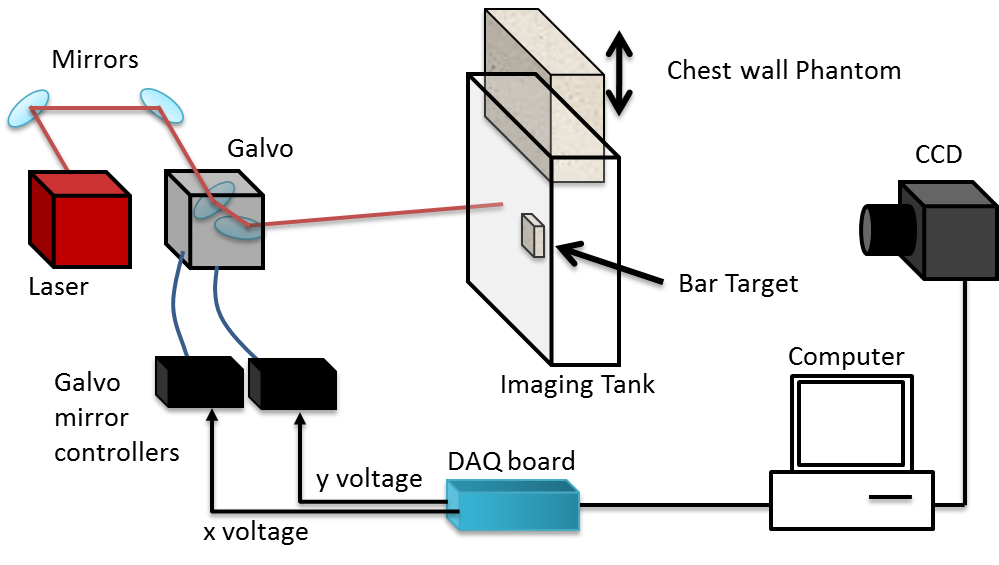
\includegraphics[width=14cm]{./figures/3_Chestwall/chestwallschem.png}
\caption[Schematic of the chest wall experiment]{Schematic of the experimental setup at the optical bench. A CW $785\,{\rm nm}$ laser source is raster scanned on one side of the imaging tank. The transmitted light on the detection plane is collected in parallel by a CCD and then binned (flexibly) for each source position.}
\label{fig:chestwallschem}
\end{figure}
\subsection{Light source}
Source illumination light is derived from a collimated $785$nm $90$mW  diode laser (Thorlabs, L785P090). The laser is coupled to a 2D galvonometer scanner (Thorlabs, GV012). The diode laser output is temperature sensitive, and therefore it is temperature controlled using a diode laser mount (Thorlabs, TCLDM9) and a temperature controller (ILX lightwave, LDT-5525) with custom cable for different pin configurations (required when using different brands for the mount and controller). The laser is current driven at $160\,{\rm mA}$ using the diode laser controller (Thorlabs, LDC500). The wavelength of the laser is $785\,{\rm nm}$. The output of the beam is collimated (Thorlabs, C140TMD-B) on the laser mount and is then focused, over a $2\,{\rm m}$ length, to a $0.5\,{\rm mm}$ spot size onto the source plane of the imaging tank.

The beam is raster scanned across this source plane of the imaging tank. Specifically, the collimated laser light is aligned with a pair of mirrors into the galvo scanner which raster scans a $35\times 35$ square grid with a $4\,{\rm mm}$ spacing covering an area of $13.6\times 13.6\,{\rm cm}^2$ on the inner side of the source window of the imaging tank. The galvo is controlled with a pair of drivers (one for each mirror). Voltages can be applied to the driver card to change the angle of the mirrors. Each mirror has a maximum angular displacement of $\pm 20^o$, and $1 \rm{V}$ moves the mirror $1^o$. Resistor pots on the driver were utilized to scale the voltage down (to $0.5 \rm{V}/1^o$) and to add an offset (as needed). A DAQ board (National Instruments, USB-6251) was used to output two distinct voltages (through its analog output channels a0 and a1) to the galvo scanner in series for each source position.

\begin{figure}[h]
\centering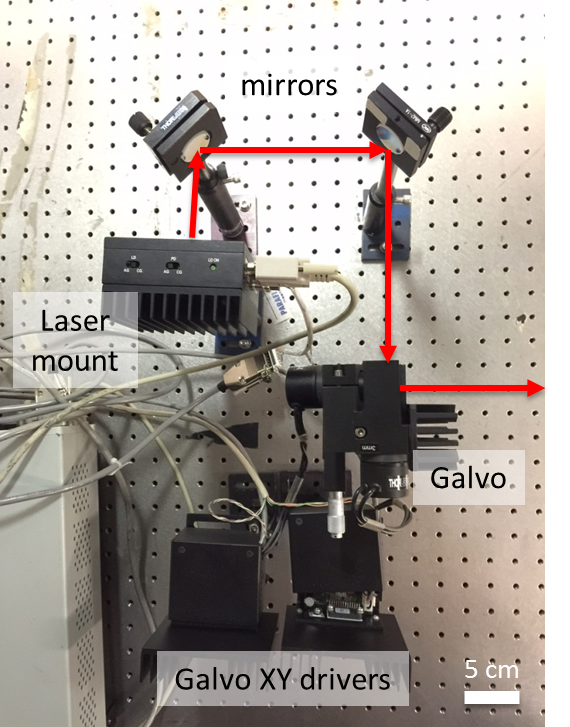
\includegraphics[width=7cm]{./figures/3_Chestwall/FSsource.png}
\caption[Photograph of the freespace laser and source position control setup]{Photograph of the laser and source position control setup. The diode laser is mounted on a TEC cooled mount with collimating lens that outputs the beam to a pair of mirrors which redirects the beam onto the galvo mirrors for scanning.}
\label{fig:FSsource}
\end{figure}

\subsection{Imaging Tank}
The imaging tank shown in Fig.~\ref{fig:chestwalltank} is designed specifically for the chest wall experiment. The tank is composed of aluminum walls on three surfaces (i.e., the bottom plate and two side plates) with acrylic windows in the input and output planes, and an opening at the top. The latter opening permits loading of Intralipid, targets and the chest wall phantom. In addition, a spigot is built into the side for easy draining and cleaning of the tank. The inner dimensions of the tank are $44\times 44\times 6\,{\rm cm}^3$. The $6\,{\rm cm}$ thickness of the tank was chosen to be close to the average compression used in our DOT clinical studies~\cite{Choe2009, Culver2003}. The unit has a removable black Delrin target holder which lines the walls of the tank, and it has evenly spaced holes that can be threaded with filamentous fishing lines to suspend various phantoms within the tank. These fishing lines hold bar targets (described in Section~\ref{sec:chestphant}). The windows are designed to be swappable and are lined with o-rings for water tight sealing. In this experiment a pair of $1/2-{\rm inch}$ acrylic windows were used. The top of the tank has optical posts that hold an aluminum plate which, in turn, holds a pair of threaded rods from which the chest wall phantom is suspended downwards.
\begin{figure}[h]
\centering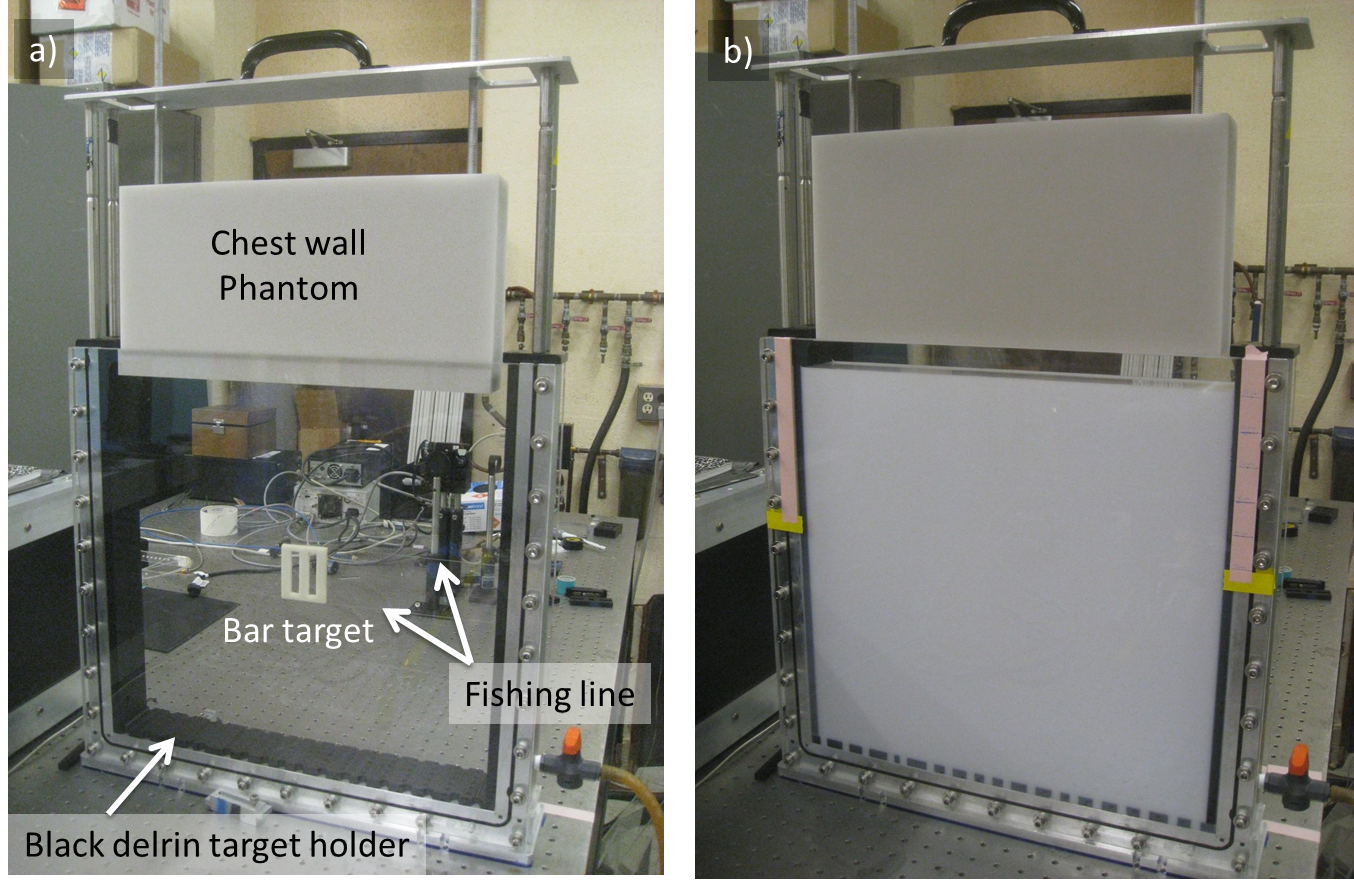
\includegraphics[width=14cm]{./figures/3_Chestwall/chestwalltank.png}
\caption[Photograph of the chest wall imaging tank]{Photograph of the imaging tank. a) The bar target is suspended below the chest wall phantom with fishing lines. b) The tank filled with Intralipid solution.}
\label{fig:chestwalltank}
\end{figure}

\subsection{CCD Detection}
For each illuminated source position, transmission data is collected on the opposite side of the tank over a $21.2\times 21.2\,{\rm cm}^2$ field-of-view (FOV) area. These data are collected with a CCD camera (Andor, DV887ECS-UV, lens $25\,{\rm mm}\ {\rm F}/0.95$). The FOV is effectively mapped to a grid of $512\times 512$ CCD pixels. This mapping yields a corresponding detected rectangular grid on the output surface of the tank with spacing $p=0.416\,{\rm mm}$. The CCD typically employed an exposure time of $500\,\rm{ms}$ at 16-bits (for a total of $2^{16}\sim64\rm{K}$ counts) with $1\times1$ binning. The total measurement time per scan was $\sim 11\,\rm{min}$.
\begin{figure}[h]
\centering
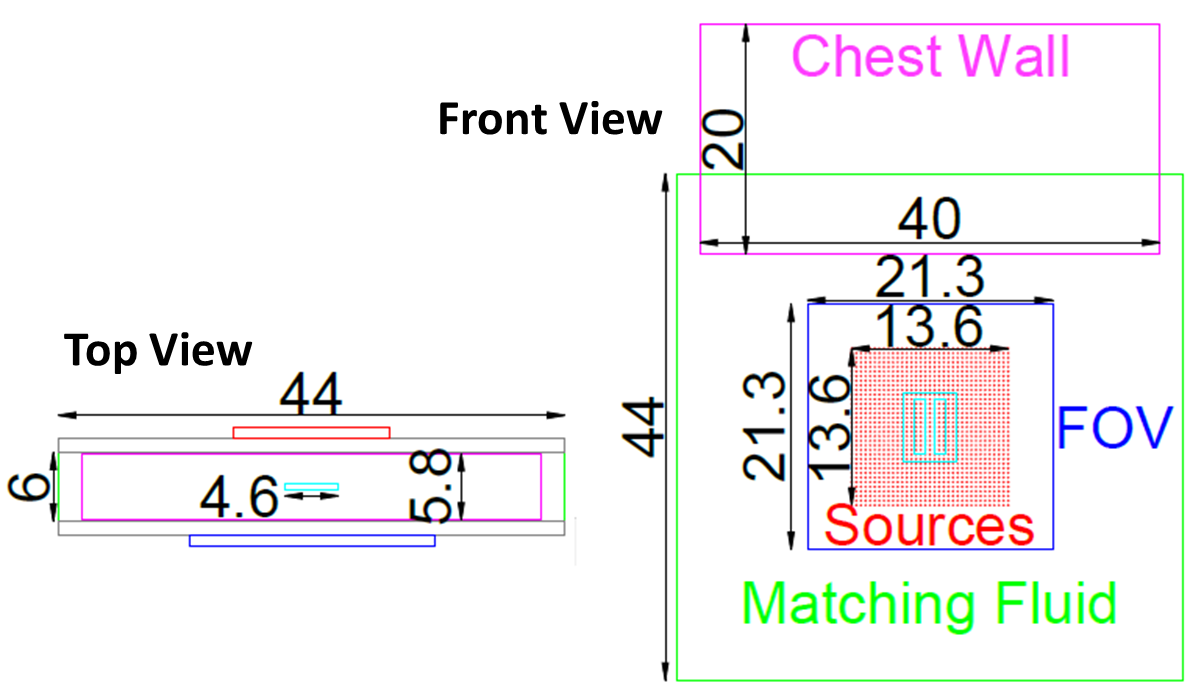
\includegraphics[width=11cm]{./figures/3_Chestwall/chestwalldim.png}
\caption[Schematic of the imaging tank with dimensions given in units of $\rm{cm}$]{Schematic of the imaging tank with dimensions given in units of $\rm{cm}$. The red sources make up a $13.6\times 13.6\,\rm{cm}$ grid within the blue $21.3\times 21.3\,\rm{cm}$ field of view of the CCD. The green dimensions are the tank size and the purple dimensions are those of the chest wall phantom.}
\label{fig:chestwalldim}
\end{figure}

\subsection{Phantoms: Bar Target and Chest Wall}
\label{sec:chestphant}
The bar target is made of silicon rubber (RTV-12, General Electric), titanium oxide (T-8141, Sigma-Aldrich) and carbon black (Raven 5000 Ultra Powder II). It has absorption coefficient $\mu_{\rm a}=0.2\,{\rm cm}^{-1}$ and reduced scattering coefficient $\mu_{\rm s}^\prime = 7.5\,{\rm cm}^{-1}$.  The tank is filled with an indian ink and intralipid solution ($\mu_{\rm a} = 0.05\,{\rm cm}^{-1}$ and $\mu_{\rm s}^\prime = 7.5\,{\rm cm}^{-1}$); these background optical properties are similar to those used in previous {\em in vitro} and clinical research. The contrast between the target and the surrounding fluid is purely absorptive with ratio of about 4. The bar target is suspended in the mid-plane of the tank ($3\,{\rm cm}$ from either surface) using the fishing line. 

A chest wall phantom (Biomimic, INO) with $\mu_{\rm a} = 0.1\,{\rm cm}^{-1}$ and $\mu_{\rm s}^\prime = 5.0\,{\rm cm}^{-1}$ and dimensions $40\times 20\times 5.8\,{\rm cm}^3$) is suspended at various distances, $d$, from the top edge of the bar target ($d=2$, $5$, $8$, $11$, $14$, $17\,{\rm cm}$) as shown in Fig.~\ref{fig:chestwallFOV} (a). The optical properties of the chest wall phantom were chosen to mimic muscle tissue~\cite{Ardeshirpour2010, Kienle1999,Taroni2003}. Thus both absorptive and scattering contrast exist between the chest wall phantom and the background fluid. The bar target and the chest wall phantom are shown in Fig.~\ref{fig:targets}.  Note that the chest wall phantom almost entirely fills the imaging tank; the clearance between the chest wall phantom and the inner surfaces of the tank is $1\,{\rm mm}$ on both sides.

\begin{figure}[t]
\centering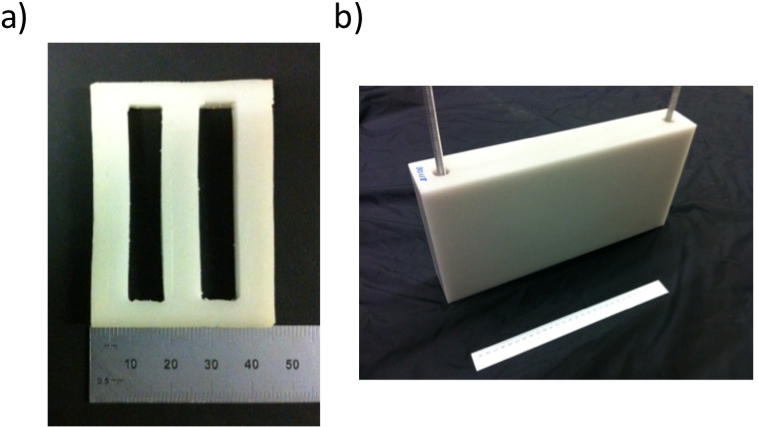
\includegraphics[width=10cm]{./figures/3_Chestwall/chestwallphant.pdf}
\caption[Phantoms used in chest wall experiment]{\label{fig:targets}
Phantoms used in the experiment. a) $6\,{\rm mm}$ thick bar target with $\mu_{\rm a}=0.2\,{\rm cm}^{-1}$ and $\mu_{\rm s}^{\prime}=7.5\,{\rm cm}^{-1}$ has slots $48\,{\rm mm}$ tall and $9\,{\rm mm}$ wide. The outer dimensions are $60\times 50\,{\rm mm}^2$. b) The chest wall phantom with $\mu_{\rm a}=0.1\,{\rm cm}^{-1}$ and $\mu_{\rm s}^{\prime}=5.0\,{\rm cm}^{-1}$.  }
\end{figure}

\section{Methods}
\label{sec:3_methods}
The experiments are straightforward. I first fill the tissue phantom tank with the background Intralipid suspension, and I collect baseline image data by cycling through each of the source positions and deriving a CCD-image output for each source position. Then I introduce the bar target into the suspension, and I insert the chest wall phantom into the suspension above the bar target (from the top). I then carry out another imaging measurement, i.e., obtaining CCD images while cycling through the source positions, with the bar target and chest wall phantom in the suspension and separated by a fixed distance. Lastly, I vary the distance between the bar target and the chest wall phantom and repeat the imaging procedure; I do this for multiple target-wall separation distances.

The data from the reference measurement and with the phantoms present are denoted by $I(\mbf{r}_d, \mbf{r}_s)$ and $I(\mbf{r}_d, \mbf{r}_s)$ (Eqns.~(\ref{eqn:Intensity1}) amd (\ref{eqn:Intensity2}) from Chapter 2) where $\mbf{r}_d$ $\mbf{r}_s$ which are the two dimensional vectors specifying the lateral positions of the detector and source on the respective surfaces of the tank. Image reconstruction is carried out using the methods described in Chapter 2 (see Section~\ref{sec:Analytic} and \ref{sec:Algebraic}). In this way, full 3D DOT reconstructions of the breast phantom and bar target are obtained as a function of the distance between the chest wall phantom and the bar target. This methodology permits characterization of the utility of the various methods in the presence of the chest wall, and it also permits exploration of selective data rejection schemes to ameliorate image artifacts. Below, I will describe this data rejection process in more detail.

In practice, a typical DOT measurement necessarily involves some rejection of data, i.e., rejection of data from source-detector pairs that are deemed unreliable or too noisy ~\cite{Blasi2007,Franceschini2007,Roche-Labarbe2010,Orihuela-Espina2010}. This data rejection could be a result of signals that are too small, uncontrolled fluctuations of the apparatus/subject, etc. In the usual approach, data are rejected based on {\em a priori} knowledge or a statistical model without specific regard for the location of the rejected source-detector pairs. In the present case, data restriction is used with a somewhat different goal to minimize systematic error effects due to the chest wall. Here particular data are rejected based solely on location. The purpose is not to suppress noise in the strictest sense, but rather to investigate the effects of imaging window restrictions and the effects of the proximity of the chest wall phantom and bar target on the quality of the image reconstructions. Importantly, the positions and distances of sources and detectors in close proximity to the chest wall are explored to determine which of them can be used, i.e., which source-detector pairs lead to reconstructions wherein the target is not significantly distorted or contaminated by chest wall systematics.

The distance between the top of the bar target and the bottom of the chest wall phantom as indicated in the figure is denoted $d$. Data is collected for $d=2$, $5$, $8$, $11$, $14$, and $17\,{\rm cm}$. The various data sets are graphically illustrated in Fig.~\ref{fig:chestwallFOV}. In Fig.~\ref{fig:chestwallFOV}(b), red lines show the positions of the lower edge of the chest wall phantom corresponding to different values of $d$ which fall within the CCD field-of-view (e.g, $d=8$, $5$, and $3\,{\rm cm}$). In this figure the source positions are shown as a small square grid of dots. Note, the image is to scale, and a slice of the sample reconstruction is superimposed with the drawing in order to indicate the target shape and position. The large dark blue square corresponds to the field-of-view (FOV) of the CCD camera. 
\begin{figure}[t]
\centering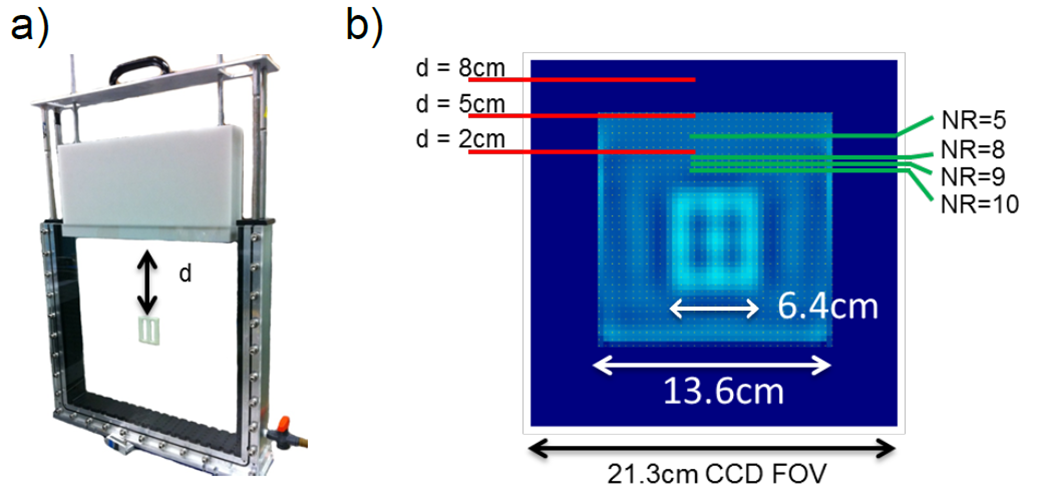
\includegraphics[width=13cm]{./figures/3_Chestwall/chestwallFOV.png}
\caption[Models for data restriction]{\label{fig:chestwallFOV}
Models for data restriction. (a) Photograph of the drained imaging tank illustrating the position the bar target with respect to the chest wall phantom. (b) Schematic of the imaging tank. (c) Illustration of the various data sets used for the reconstructions. The dark blue square is the CCD FOV; the inner light blue square indicates the reconstruction region. White dots in a square grid indicate the source positions. To illustrate the target shape and position, a slice of a sample reconstruction is superimposed with the drawing. Red lines indicate the three lowest positions of the chest wall phantom (other positions are outside of the CCD FOV), and the green lines illustrate the restricted data sets wherein all the sources and detectors situated above a given green line have been discarded.}
\end{figure}

The linear reconstruction techniques (analytical and algebraic) discussed in Section~\ref{sec:linearrecon} are applied to the experimental data obtained using the apparatus described above. These techniques are able to handle large data sets and permit comparison to previous work \cite{Konecky2008a}. The maximum number of independent source-detector pairs is $(512\times 35)^2\simeq 3.2\times 10^8$. However, only a fraction of this data (albeit still a large data set) was used in the reconstructions. Some data was eliminated by ``windowing'' (i.e., in the algebraic image reconstruction); other data were eliminated by a relatively sparse sampling of the detectors (e.g, in the algebraic reconstructions, every second detector was used), and still other data were eliminated by numerical data restrictions (described below). Thus the maximum data set utilized for reconstruction (in this case, for the algebraic reconstruction) was still very large, i.e., it consisted of $\simeq 2\times 10^7$ measurements.

In obtaining algebraic reconstructions, the reconstructed volume was divided into cubic voxels. The voxel size $h$ was taken to be equal to 8 CCD pixels $p$. Thus, $h=8\times 0.416\,{\rm mm}\simeq 3.3\,{\rm mm}$. The grid consisted of $41\times 41$ voxels in the lateral direction and 17 voxels in the depth direction. Therefore, the discretized volume was a parallelepiped with the dimensions $13.6\times 13.6\times 4.3\,{\rm cm}^3$ consisting of $N=21853$ voxels. This parallelepiped was positioned from each surface of the slab. The target was situated approximately in the middle of the discretized volume. The computation of $A^*A$ (see Section.~\ref{sec:Algebraic}is greatly accelerated by sampling the detectors for the purpose of computing the product $A^*A$, but not for computing the projection $A^*\phi$. In this way, the number of data points and the voxels used is not reduced but the computation time is shortened dramatically with no or minimal effects on the image quality. Indeed, we have verified that $A^*A$ can be computed by using the method in Ref.~\cite{Markel2005} in about 2 hrs with very minimal degradation of image quality.

An additional feature of the algebraic method is that it does not require that the set of detectors used be independent of the position of the source. We have taken advantage of this feature and have excluded the data points that are very far off-axis. Specifically, for each source, we have used only such detectors that are situated no further from the axis of the source than a given radius $R$. We have used $R=6.25\,{\rm cm}$, so that $R$ is slightly larger than the width of the slab ($6\,{\rm cm}$). The justification for discarding the strongly off-axis data points is that these measurements contain predominantly noise.

The critical sources and detectors for the chest wall problem are those whose location is physically near the chest wall. An important question concerns how close to the chest wall one can collect data and maintain good image fidelity. Thus, for the present study, numerical data restriction involved removing all sources and detectors above one of the green lines shown in Fig.~\ref{fig:chestwallFOV}(c). In the case of algebraic reconstruction, sources \textbf{and} detectors above these lines were simply not used; thus no additional approximation was made.  In the case of the analytical reconstruction (i.e., using analytic inversion formulas), data points cannot be excluded even for points above the green line. Rather it was assumed that the corresponding data points for these source-detector pairs ($b_m$) are zero ($I=I_0$), i.e., no change in intensity from the reference measurement (see Section.~\ref{sec:rytov} in Chapter 2). In the upcoming discussion, $NR$ denotes Numerical Data Restriction and is defined as the number of the “source row” (counting from top to bottom) above which no sources and/or detectors are included in the reconstruction. For example, $NR=5$ excludes the four top-most lines of sources and all detectors that lie above the fifth line of sources. In the test reconstructions, $NR=5, 8, 9, 10$ were used; for each value of $NR$, an image reconstruction was performed with all available values of $d$. Table 1 summarizes the subsets of data used for each value of $NR$. 
\begin{table}[t]
\centering\caption{Data Restriction Sizes.}
\begin{tabular}{|c|c|c|}
\hline 
Numerical Data Restriction ($NR$) & Number of sources & 
Number of distinct \\
&& source-detector pairs \\ \hline
No restriction & $35\times35=1,225$ & $20,591,492$ \\
           $5$ & $35\times31=1,085$ & $16,479,152$ \\
           $8$ & $35\times28=980$  & $14,661,145$ \\
           $9$ & $35\times27=945$  & $14,074,728$ \\
          $10$ & $35\times26=910$  & $13,457,507$ \\ \hline
\end{tabular}
\end{table}

\section{Results}
\label{sec:3_results}
In this section we report on the application of analytical and algebraic reconstruction methods (Section~\ref{sec:Analytic} and \ref{sec:Algebraic}) to the data sets collected as described above. The reconstruction results are displayed. In particular, I will show various reconstructions of the bar target with the chest wall at different distances $d$. 

The reconstructed image contrast in all figures of this section is $x(\mbf{r}) = \alpha(\mbf{r}) / \alpha_0+1$ where $\alpha = c\delta\mua$. Note we have redefined $\alpha$ (different from the more general form in Section~\ref{sec:rytov}, Chapter 2) for this experiment where only the absorption was reconstructed and scattering was assumed to be constant. This function is non-negative since the medium does not amplify light. However, the image reconstructions will employ various approximations. Sometimes a particular approximation can produce an unphysical negative value of absorption in the reconstruction; these volume elements are shown in the figures by the color black (note, the same color scale is used for all images). In practice, the occurrence of negative absorption can be avoided by using a positivity constraint in the algebraic reconstruction method. The positivity constraint can be directly incorporated into the conjugate-gradient descent algorithm, which was used to invert the matrix $A^*A$. However, in practice the areas of negative absorption appear mostly for the analytic image reconstruction method, and it is not possible to incorporate the positivity constraint into the analytic inversions. By contrast, the algebraic reconstructions have produced either no areas of negative absorption, or artifacts so severe (e.g., when $d=2\,{\rm cm}$ and no numerical data restriction is used) that the positivity constraint was unnecessary. Since no situation occurred wherein the positivity constraint was simultaneously numerically sensible and useful, it was not employed for the images shown in this chapter.

\subsection{Analytical Reconstruction Results}
Reconstructions of the central slice of the medium ($3\,{\rm cm}$ from either of the slab surfaces) obtained with varying values of $d$ and various numerical data restriction ($NR$) are shown in Fig.~\ref{fig:fastcenter}. It is apparent that the analytical inversion with no data restriction (the topmost row of images) produces severe image artifacts when chest wall is at distances of $d=2\,{\rm cm}$ and even $d=5\,{\rm cm}$ away from the target. To remove artifacts associated with the chest wall completely, $NR=10$ is required. The data restriction with $NR=5$ results in a reasonable, yet suboptimal, image quality when $d=5\,{\rm cm}$, but not when $d=2\,{\rm cm}$. 
\begin{figure}[h]
\centering
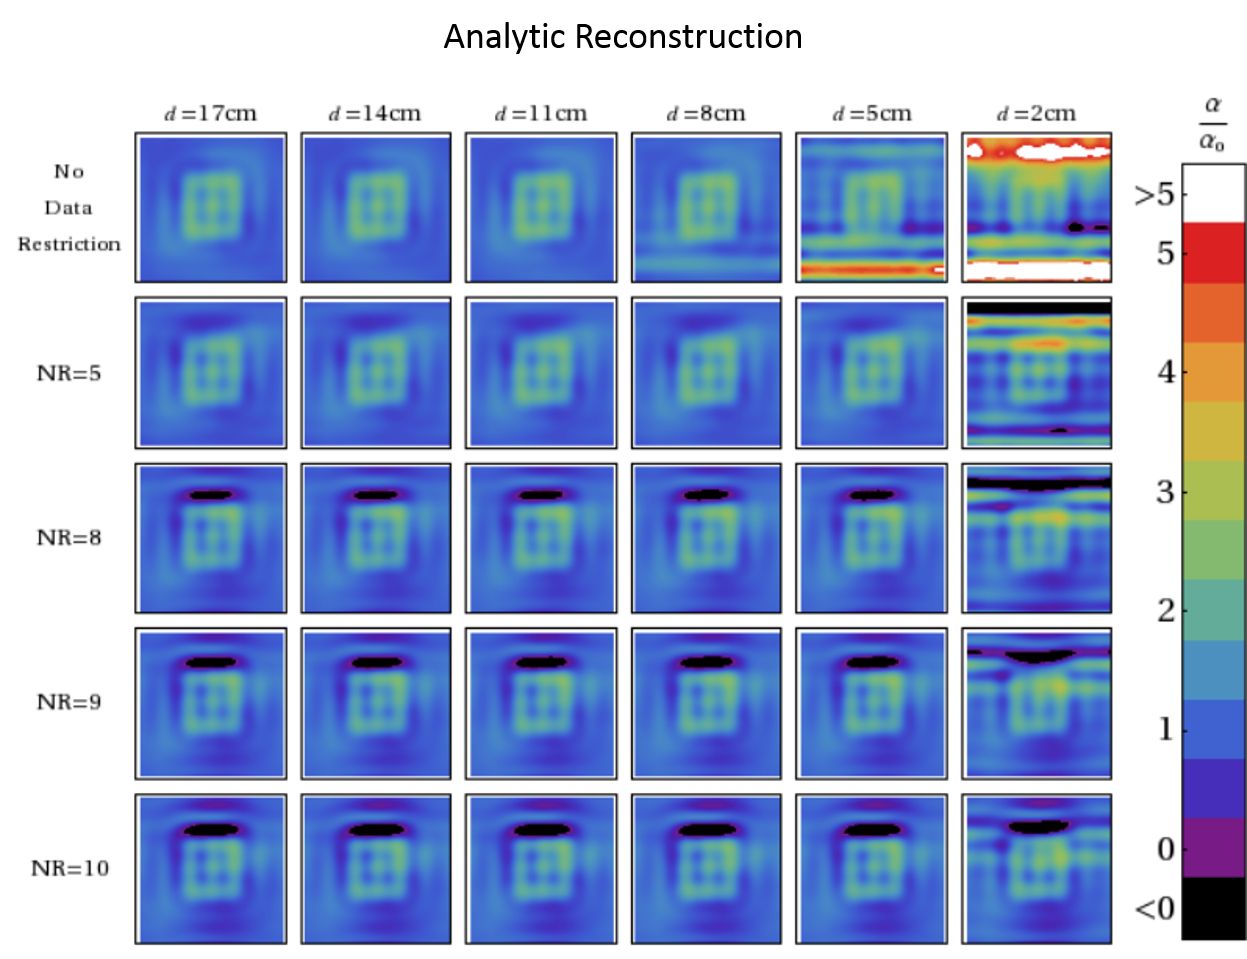
\includegraphics[width=0.9\textwidth]{./figures/3_Chestwall/fastcenter.png}
\caption[Images of the central slice obtained by analytical reconstruction method]{\label{fig:fastcenter}
Images of the central slice obtained by analytical reconstruction method. Different columns show data obtained with the chest wall phantoms at different distances $d$ from the bar target. Different rows of images correspond to different data restrictions $NR$, as indicated.}
\end{figure}

\begin{figure}[htbp]
\centering
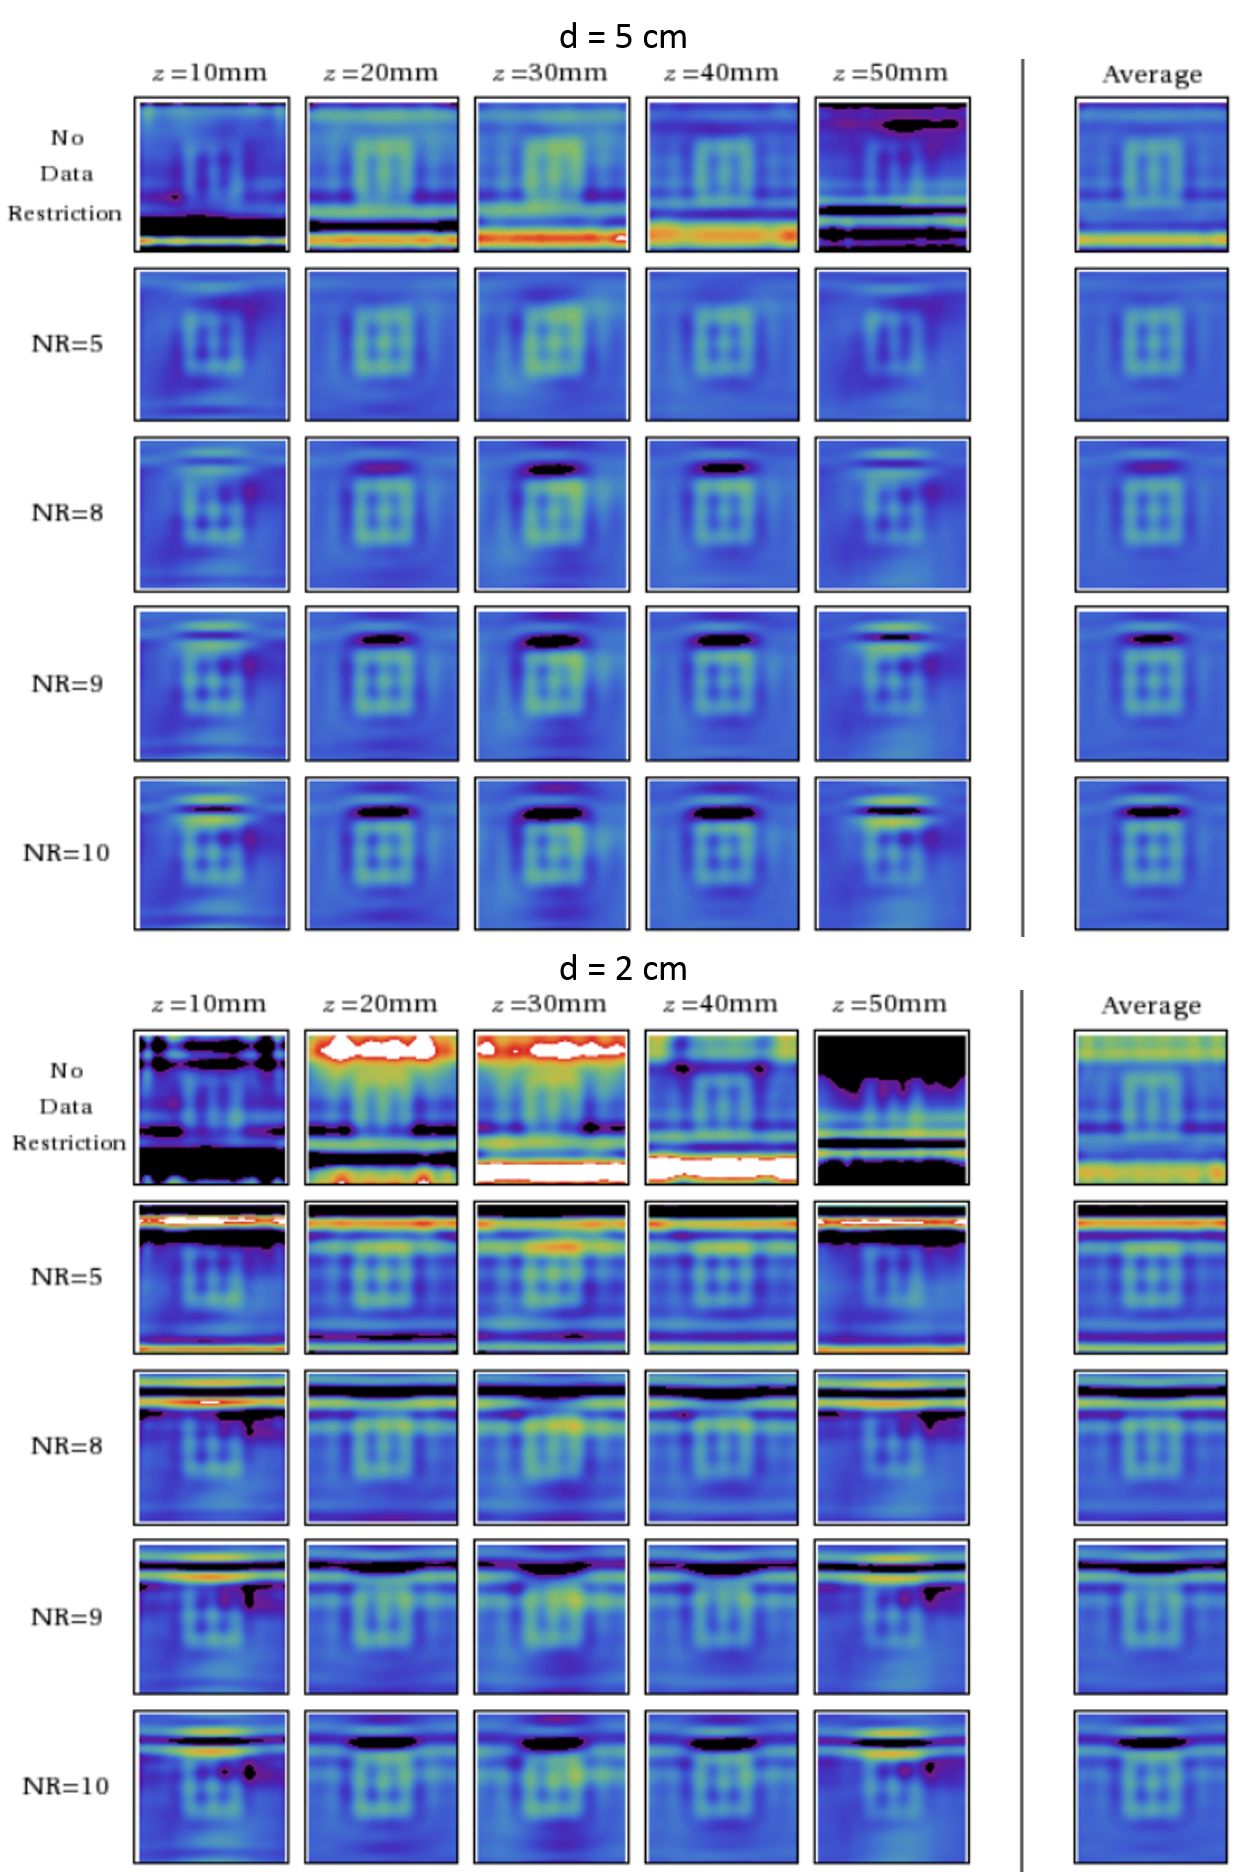
\includegraphics[width=0.9\textwidth]{./figures/3_Chestwall/anaslices.png}
\caption[Analytical reconstruction images at various depths]{\label{fig:slices_analytical}
Slices through the medium drawn at different depths (from plane of sources). The analytical inversion reconstruction method used for $d=5\,\rm{cm}$ and $d=2\,\rm{cm}$.}
\end{figure}
Interestingly, when the data restriction $NR = 8, 9, 10$ is used in conjunction with the analytical reconstruction, it yields an additional image artifact, which is unrelated to the chest wall phantom. To see that this is true, consider the images for $d=17\,{\rm cm}$, which are not affected at all by the chest wall phantom, yet exhibit the additional artifact just mentioned. This artifact is evident as a black area wherein the reconstructed absorption coefficient is negative; therefore, it is outside of the physically-allowable range. Thus, it is reasonable to conclude that reconstructing the target via the analytical reconstruction method is feasible, especially with the use of the appropriate data restriction, but additional image artifacts can arise where the absorption is underestimated. 

In fact, the appearance of this artifact can be understood. As mentioned above, the data restriction used with the analytical reconstruction amounts to assuming that the truncated data points are zero. In other words, if it is assumed (even in the presence of the target) that the truncated source-detector pairs would have measured the same intensity as in the homogeneous slab, then $I(\mbf{r}_d,\mbf{r}_s) = I_0(\mbf{r}_d,\mbf{r}_s)$ for the truncated source-detector pairs (see Section~\ref{sec:rytov}, Chapter 2). The reconstruction algorithm seeks a contrast function $\delta\alpha(\mbf{r})$, which is compatible with this assumption.  For a purely absorbing target, however, the actual intensity $I(\mbf{r}_d,\mbf{r}_s)$ is smaller than $I_0(\mbf{r}_d,\mbf{r}_s)$ when at least one of the points $\mbf{r}_d,\mbf{r}_s$ is located not too far from the target (in the lateral direction) due to increased optical absorption. Whenever such data points are discarded, an artifact with negative $\delta\alpha$ is produced by the reconstruction algorithm to compensate for the absorption in the target. It can be seen that this artifact is located between the target and the region of source-detector pairs, which have been discarded. Of course, this analysis applies to the case when the position and optical contrast of the target is known.  In general, it may be difficult to predict the position of this artifact or to distinguish it from a true occurrence of negative $\delta\alpha$. There may also be a spatial overlap of the artifact and a true inhomogeneity.

\subsection{Algebraic Reconstruction Results}
In the algebraic reconstructions in Fig.~\ref{fig:algcenter} with the unrestricted data set, the image quality is still poor when the chest wall is to close. However, when the data restriction is gradually introduced these artifacts disappear. In the case $NR=10$ and $d=2\,{\rm cm}$ (the image in the bottom right corner), the target is clearly visible, and the image quality is about the same as with the use of the unrestricted data set and $d=17\,{\rm cm}$. Thus, introduction of data restriction does not result in substantively additional image artifacts or image quality degradation when the algebraic method is used.
\begin{figure}[h]
\centering
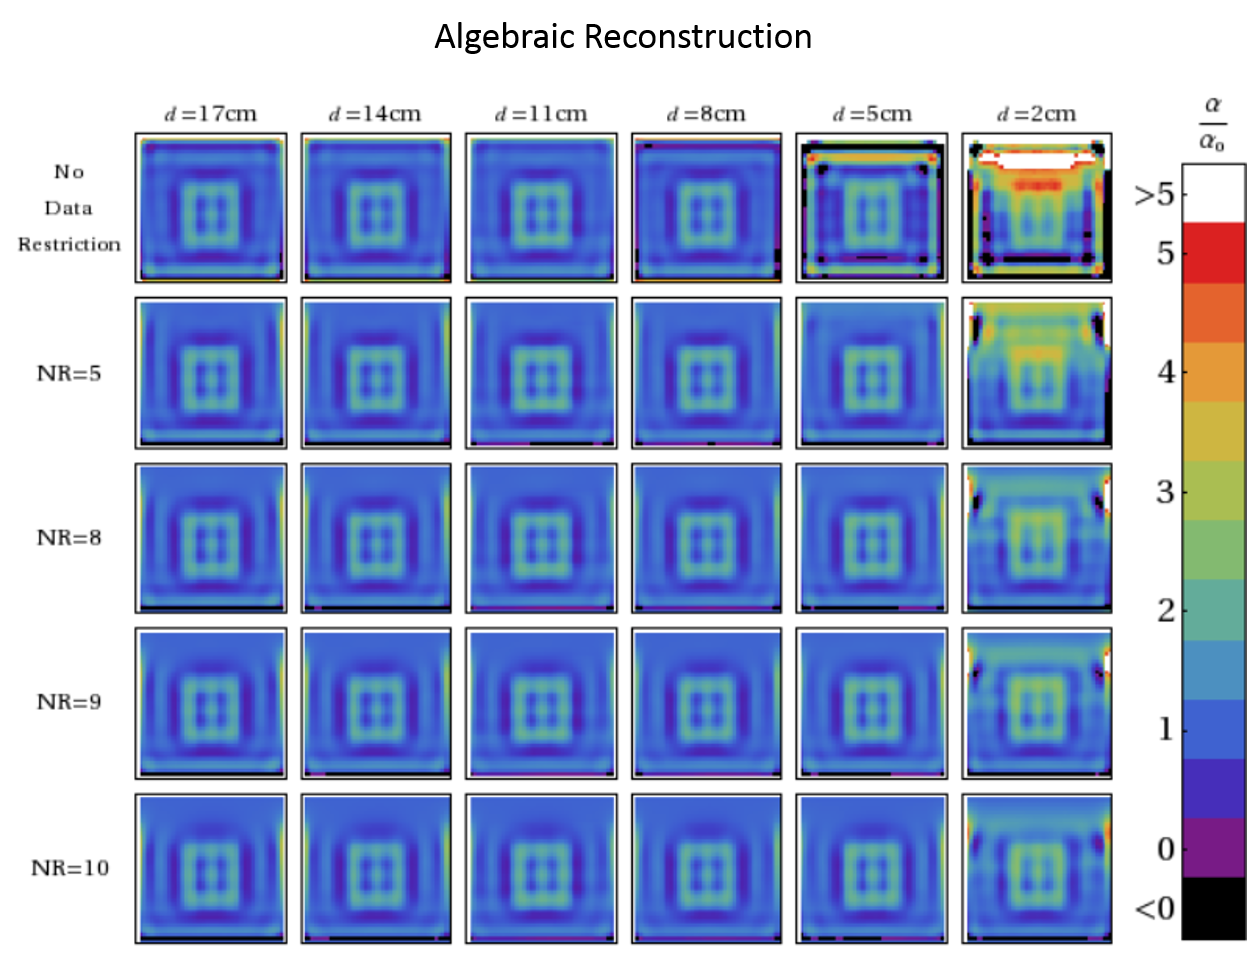
\includegraphics[width=0.9\textwidth]{./figures/3_Chestwall/algcenter.png}
\caption[Images of the central slice obtained by algebraic reconstruction method]{\label{fig:algcenter}
Images of the central slice obtained by algebraic reconstruction method. Different columns show data obtained with the chest wall phantoms at different distances $d$ from the bar target.  Different rows of images correspond to different data restrictions $NR$, as indicated.}
\end{figure}
\begin{figure}[p]
\centering
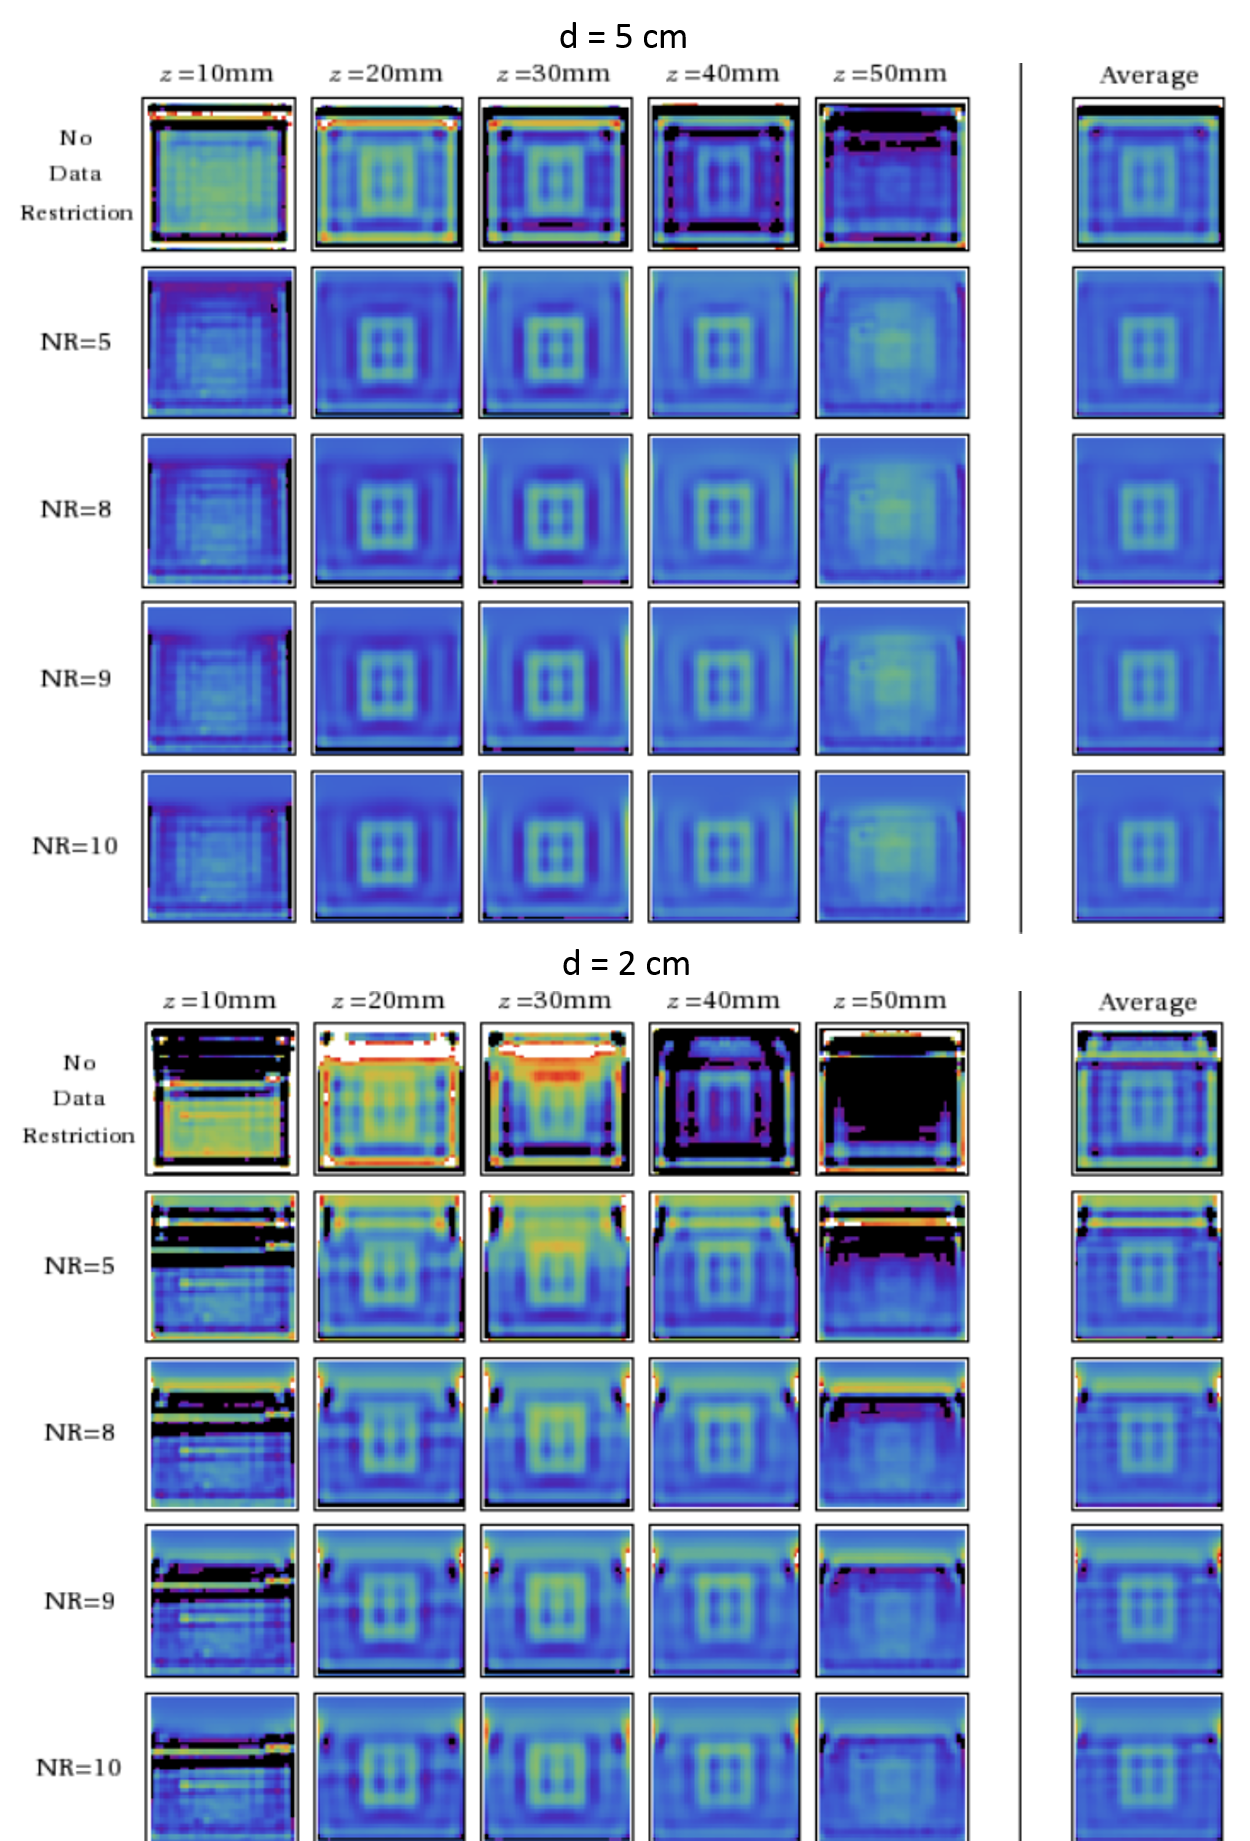
\includegraphics[width=0.9\textwidth]{./figures/3_Chestwall/algslices.png}
\caption[Algebraic reconstruction images at various depths]{Same as in Fig.~\ref{fig:slices_analytical}, but I this case the images are obtained by algebraic reconstruction}
\label{fig:slices_numerical}
\end{figure}

\subsection{Comparison of Reconstruction methods and Projection Images}
Figs.~\ref{fig:slices_analytical} and \ref{fig:slices_numerical} show slices drawn through the medium at different depths. Fig.~\ref{fig:slices_analytical} displays the results of the analytical image reconstruction for $d=5\,{\rm cm}$ and $d=2\,{\rm cm}$ and Fig.~\ref{fig:slices_numerical} displays analogous data obtained by the algebraic reconstruction. In addition, in the right-most column of images, a different kind of image is shown; these images are reconstructions derived by averaging the full 3D tomogram over the depth of the sample (that is, averaging over the different slices). Note that, in all cases $13$ slices in the tomogram are separated by the distance of $\approx 3.328{\rm mm}$, with the central slice located exactly in the mid-plane of the slab. The ``average'' reconstruction (in the right-most column of the images) was obtained by computing the arithmetic average of all $13$ slices.

These averaged (``projection'') images correspond to the usual radiological projections obtained with a parallel beam of X-rays. Interestingly, the qualitative conclusions that can be drawn from Figs.~\ref{fig:slices_analytical} and \ref{fig:slices_numerical} are largely the same as given above for the full tomograms. The analytical reconstruction produces reasonable image quality for the smallest chest wall-target separation $d=2\,{\rm cm}$ and $NR=10$, but at the cost of an additional image artifact. The algebraic reconstruction is free from this artifact, but it underestimates the image contrast relative to the analytic method (see below). The depth resolution is slightly better in algebraic reconstructions but, overall (i.e., in both methods), depth resolution is worse than lateral resolution. This effect is typical for DOT images.

Another interesting feature can be discerned from both types of image reconstructions. Generally, the projection images discussed above are more stable and exhibit reasonable quality even when the individual slices contain substantial artifacts. For example, consider the $d=2\,{\rm cm}$ algebraic reconstructions without data restriction (Fig.~\ref{fig:slices_numerical}). Even though all slices drawn through the medium are corrupted by the artifacts associated with proximity of the chest wall phantom, the projection image shows the target clearly. Moreover, the edge of the chest wall phantom is also clearly visible at the correct location. I was surprised, and indeed our group was surprised by this result. It can be useful in situations when the depth resolution is not of essence. However, it should be emphasized that obtaining the projections still requires knowledge of the three-dimensional distribution of the absorption coefficient; the projections cannot be computed or measured directly without such knowledge.

Finally, note that in both types of image reconstructions, an underestimation of the contrast for the target phantom is observed compared to the expected value. This underestimation can be attributed to the poor transverse (depth) resolution of the three-dimensional reconstruction which results in the ``spreading'' of the contrast in that direction. Indeed, consider the depth-integrated contrast, $H(x,y) = \int \left[\alpha(x,y,z) / \alpha_0 - 1 \right] {\rm d}z$, where $x$, $y$ are the coordinates in the plane of the slab and $z$ is the transverse (depth) coordinate. Inside the target, $\alpha(x,y,z) / \alpha_0 \simeq 4$ and the target thickness in the transverse direction is $\Delta z=0.6\,\ {\rm cm}$. Therefore, the actual value of $H$ for a line passing through the target and perpendicularly to the slab surface is $H\simeq 1.8\,{\rm cm}$. In the reconstructed images, the transverse thickness of the target is overestimated and is equal, approximately, to $2\,{\rm cm}$ while the quantity $\alpha(x,y,z)/\alpha_0$ is underestimated and is equal, approximately, to 2. By using the reconstructed values to estimate the integrated contrast, one obtains $H\simeq 2\,{\rm cm}$, which is reasonably close to the actual value. Again, this effect (and analysis scheme) can be useful in practice.

\section{Summary}
\label{sec:3_summary}
The aim of my experiment was to assess the effects of the chest wall on DOT and ultimately to explore methods to mitigate the effect of the chest wall on DOT reconstructions. Both the analytical and the algebraic data-intensive linearized image reconstruction methods produce reasonable results, provided the data points are appropriately restricted to exclude measurements that are strongly influenced by the chest wall. Under these conditions, an absorbing target with sub-ccentimeter features can be clearly reconstructed in the middle of a $6$ cm slab, even when the chest wall is only $2$ cm from the target. This situation corresponds to breast tumors very near the chest wall. Specifically, good images of the target were obtained even in the presence of a large chest wall phantom that introduces significant nonlinearities into the inverse problem,  i.e., due to its larger absorption coefficient compared to the background as well as its large size. 

A data restriction condition was discovered such that the presence of the chest wall phantom imposes minimal artifacts or distortions in the image. The image quality of the projections was good and it would be of interest to explore the utility of these reconstructions for improved 2D imaging or improved quantification or in combination with other 2D modalities. The performance of both algebraic and analytic image reconstruction methods were then compared under this condition and, while neither method is perfect, it appears that a role for both methods in DOT exists, the choice depending upon the particular clinical application. For example, the analytical method provides faster reconstruction while suffering from minor artifacts and flexibility. While the algebraic reconstruction method provides slightly better image quality, it will require a library of weight matrices for faster inversion that would have to be stored ahead of time before measurements (see Section~\ref{sec:Algebraic}. We hope to build on these techniques in the future, especially by implementing non-linear approaches or by modification of the Green's function used to account for the chest wall region and its optical properties.
\chapter{CCD-based Multispectral Frequency-Domain DOT of Breast Cancer}
\section{Introduction}
Diffuse optical tomography (DOT) of the breast has a long and successful history at Penn where several instruments have been developed to translate DOT techniques to the clinic \cite{corlu_03_1,culver_03_3,Holboke2000,Ntziachristos1999,Ntziachristos2001,Ntziachristos2000,Ntziachristos2002,OLeary1996,Zhu1999}. My work builds on and improves upon these works while addressing some critical limitations the previous generation of the DOT breast imager (Gen2) used in many successful clinical studies \cite{choe_05_1,choe_09_1,corlu_07_1,corlu_03_1,corlu_05_1,culver_03_1}. The new DOT imager (Gen3) includes several feature upgrades: 1) multispectral frequency-domain measurements in the transmission geometry using heterodyne measurement techniques, 2) addition of profilometry systems for enhanced breast segmentation and 3) deployment of the largest clinical source-detector pair datasets for improved 3D reconstructions 4) as well as an improved clinical patient interface. In this chapter, I provide an overview of the Gen3 instrument design and its new features, followed by characterization measurements with tissue simulating phantoms. Finally, clinical results from cancer patients will be shown.

\section{Previous Breast Imaging Device (Gen2)}
The previous DOT imaging device shown in Fig. \ref{fig:gen2pic}. The Gen2 DOT imaging device images the breast in transmission through parallel plate compression geometry. The device illuminates breast tissue with multi-spectral CW light while detecting the transmitted light with a CCD. In addition, the the bulk tissue optical properties is determined using frequency-domain measurements in the remission geometry. The measurement is made with the patient lying prone on a flat bed with her breast inserted inside a recessed box. This box has a grid of source fibers on one side (source plate) with a window on the other (detector plate). The source plate is moved axially to softly compress the breast between the source and detector plates. The box is then filled with a matching fluid with optical properties similar to average human breast tissue before measurement. The matching fluid consists of water, india ink (for absorption) and intralipid (for scattering).
\begin{figure}[ht]
\begin{center}
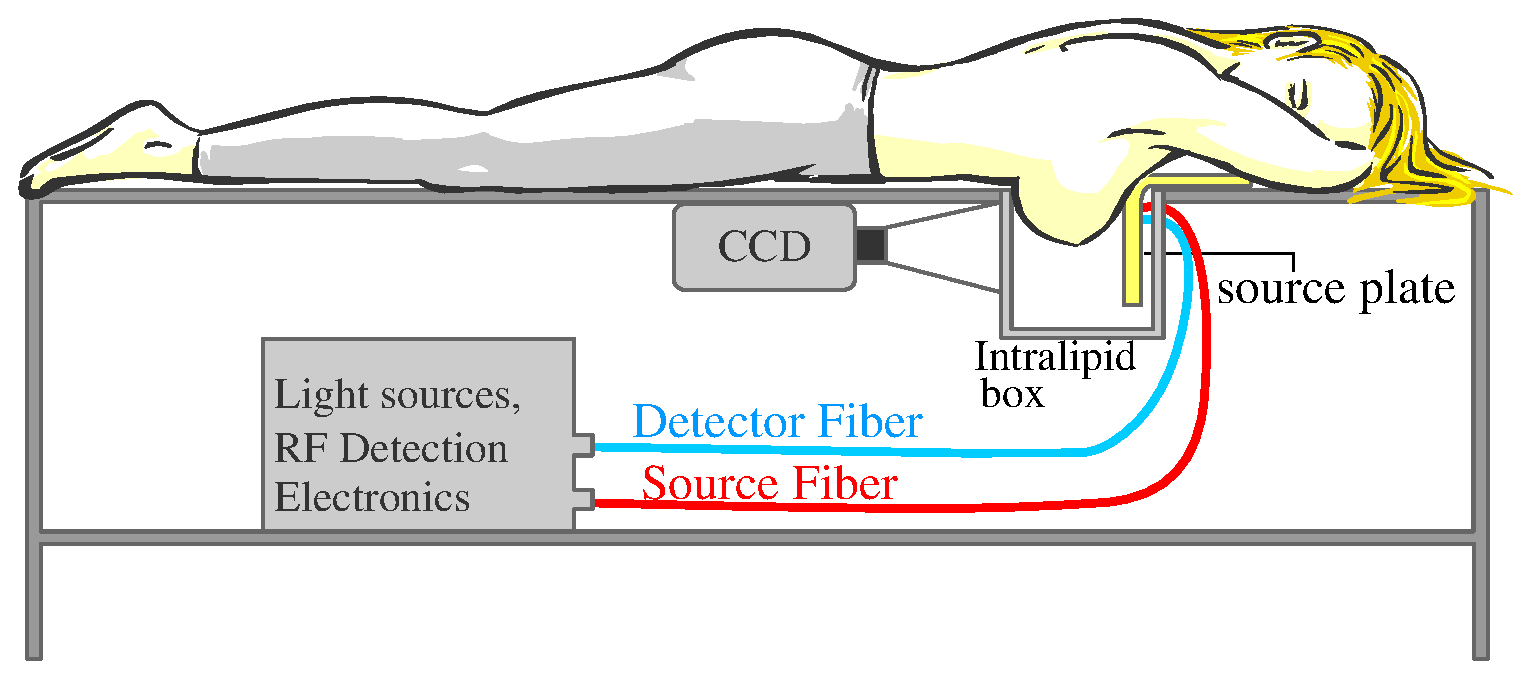
\includegraphics[width=10.5cm]{./figures/4_Gen3/gen2schem.eps}
\caption{Schematic of the previous generation breast scanner.}
\label{fig:gen2schem}
\end{center}
\end{figure}
The source plate has 45 fiber positions arranged in a 9x5 square grid with a spacing of 16 mm between nearest neighbors. The sources are measured in series using cascading optical switches (DiCon Fiber Optics, Richmond, CA). At each source position six measurements are made at varying wavelengths (650, 690, 750, 785, 830, 905 nm) using fiber-coupled laser diodes. On the detection side, a CCD camera (Roper Scientific, Trenton, NJ, VersArray:1300F) collects the light that exits in the transmission geometry focused on the detection window. A image is obtained for for each source and laser combination with an exposure time of 500 ms. From each image a  A 24$\times$41 grid of 984  decimated set is selected from the CCD after 2x2 hardware binning of the pixels. For the frequency-domain remission measurements, four out of the six lasers are modulated at 70MHz. At these wavelengths measurements are made with additional grid of 3mm detector fibers arranged on the source plate in a 3x3 grid with 16 mm spacing. The light from these fibers are collected by an avalanche photodiode for homodyne frequency-domain measurements.

A lot was learned from this device and it informed the design and development of the current DOT breast imager. In general, it is difficult to reduce the cross-talk of absorption and scattering with CW measurements as both can attenuate the level of detected light between a source and detector in a diffuse medium. We showed some success of mitigating this with multi-spectral measurement, but this can be improved upon with frequency-domain measurements. The breast was also compressed in the axial geometry required comparisons of the DOT to MRI images--which are taken in the saggital geometry more difficult.

\section{Clinical Breast Imaging Device (Gen3)}
The Gen3 breast imaging device primarily improves on the previous device through the use of multispectral and frequency-domain illumination and a CCD based heterodyne detection that  improves quantification and separation of absorption and scattering during 3D reconstruction of DOT data. Using a CCD camera for detection allow us to also collect a large number ($10^6$) of source detector pairs in parallel for improved resolution. In addition a supplemental pair of profilometry imaging systems were designed and built (discussed in Sec. \ref{sec:profilometry}) to provide 3D surface information about the breast shape. This 3D breast shape improves segmentation of the reconstruction volume of the breast. Finally, significant effort was made to build a clinical grade device with a patient interface that maximized comfort and minimized movement during our measurement. Software for the device was also developed to enable simple and streamlined operation by our clinical collaborators.
\begin{figure}[ht]
\begin{center}
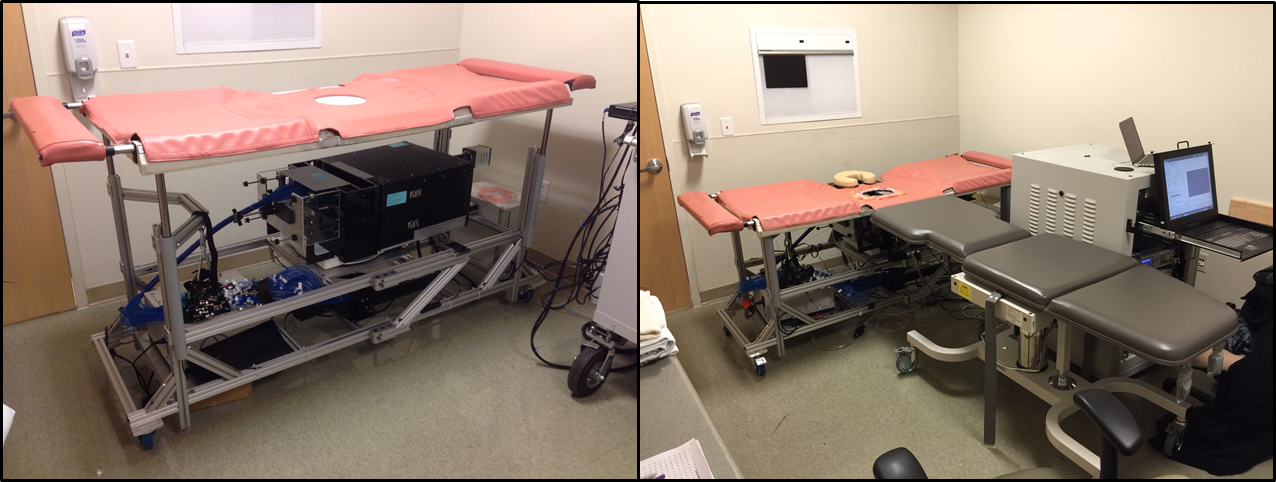
\includegraphics[width=14.5cm]{./figures/4_Gen3/gen3pic3.png}
\caption{Then breast imaging device in the mammography wing of Perelman Center for Advanced Medicine at the University of Pennsylvania (replace later)}
\label{fig:gen3pic}
\end{center}
\end{figure}
\begin{figure}[ht]
\begin{center}
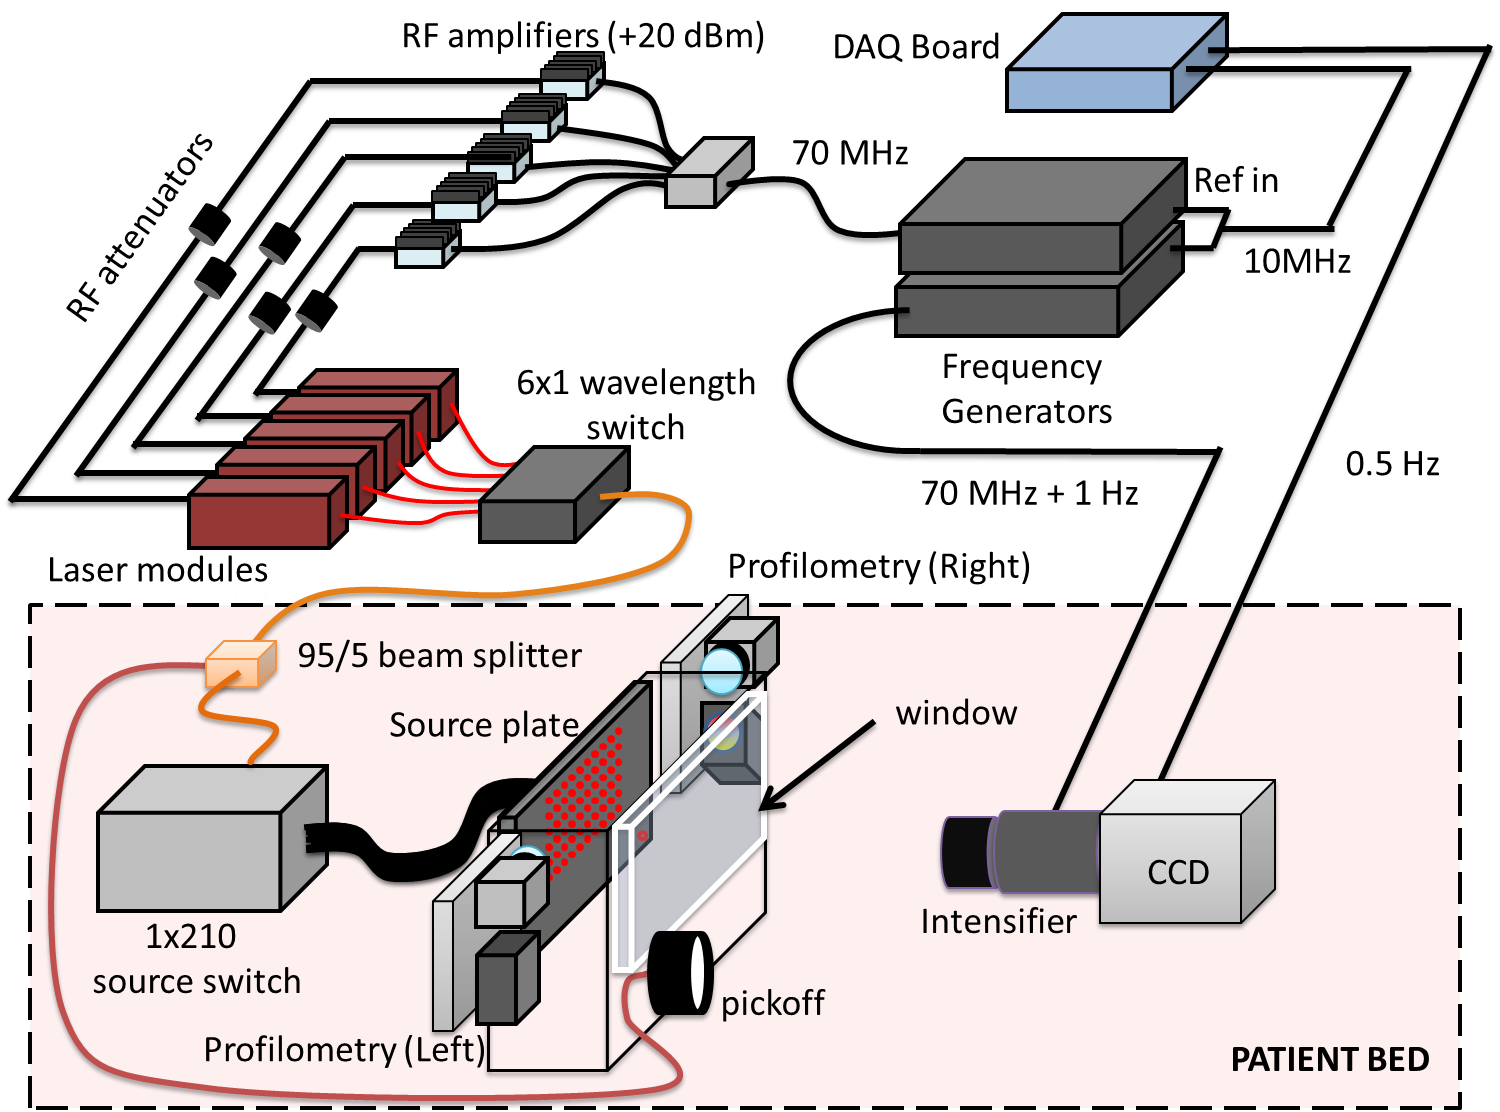
\includegraphics[width=14.5cm]{./figures/4_Gen3/gen3schem.png}
\caption{Schematic of the clinical DOT breast imaging device}
\label{fig:gen3schem}
\end{center}
\end{figure}
The schematic for the clinical breast imaging prototype that I built is shown in Fig.~\ref{fig:gen3schem}. The patient lies prone on a modified biopsy bed while one breast is centered and sagittally compressed between the source plate and window in the breast tank. Typical thickness of compression varies between 56mm and 70mm. The tank is filled with a solution of intralipid and india ink mixture to match the optical properties of tissue of the patient in the NIR wavelength range.

The breast imager comprises of several key components. Briefly, a laser system encompasses optics and electronics for generating frequency-modulated light source at various NIR wavelengths. This light is put through a custom switch to one of 209 source positions inside a breast tank where a breast is inserted. The breast tank has two sets of profilometry cameras and projectors for 3D segmentation. Lastly, we have a gain-modulated detection using an image intensifer mounted CCD. I wil now discuss each of these subsystems in detail in the following sections.

\subsection{Laser System}
Illumination is provided by laser diodes with the wavelength of $660$, $690$, $785$, $808$, and $830\,{\rm nm}$ . Table \ref{fig:lasertable} provides detailed characteristics of each laser module (Fig.~\ref{fig:laserpic}). The laser diodes are mounted on a custom copper block for a TEC cooler and cooled to $-13^{\circ}{\rm C}$. Each laser diode is driven and temperature controlled by a dedicated ILX mainframe module (instrument info). The lasers are amplitude modulated at $70\,{\rm MHz}$ using a an RF signal from a frequency generator (Rhode and Schwartz, SMB100). More specifically, the $70\,{\rm MHz}$ RF signal from the frequency generator is combined with the DC current from the ILX driver for each laser with ??? (minicircuit). The DC and RF voltage input for each laser was optimized using RF amplifiers (?), RF attenuators (?). The laser driver current is optimized for the best modulation depth ($>80 \%$) and a sinusoidal waveform. The frequency modulated light from each fiber coupled laser is then coupled to a 6x1 100 $\mu m$ core optical switch (Optojenna) which allows the system to switch wavelengths in series.
\begin{figure}[ht]
\begin{center}
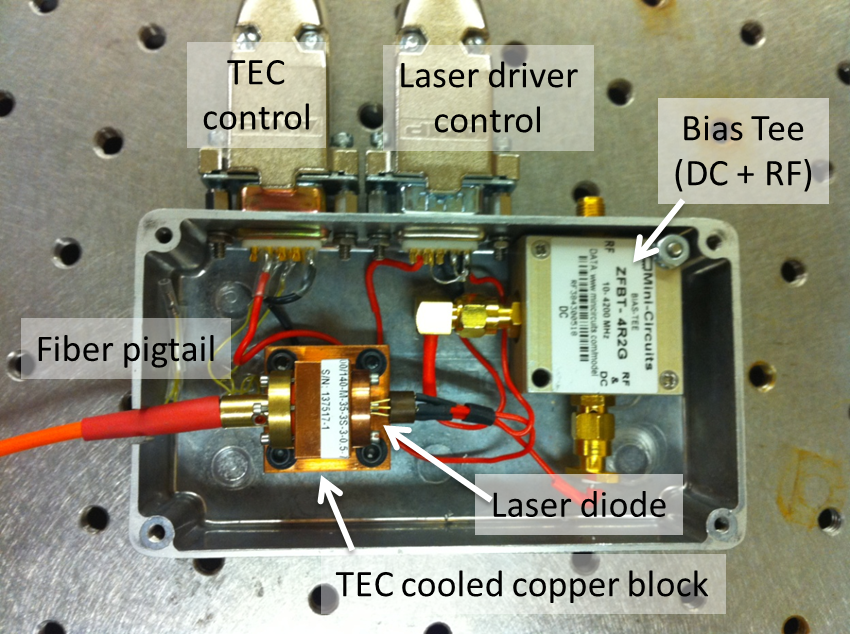
\includegraphics[width=10cm]{./figures/4_Gen3/laserpic.png}
\caption{Schematic of the clinical DOT breast imaging device}
\label{fig:laserpic}
\end{center}
\end{figure}

\subsection{Source Position Switch and Source Plate}
The output fiber from wavelength switch is connected in series to a $95/5$ fiber beam splitter with the $5\%$ going to the the pickoff--to be discussed in Sec. \ref{sec:datanorm}--and $95\5$ going to a custom 1x210 channel optical galvo switch. Switching through 210 channels with a conventional cascade of switches used in the previous system based on mechanical or prism switch mechanisms is costly, slow, and have high throughput losses. The custom switch collimates light from a $100\,\mu{\rm m}$ input fiber and uses galvo controlled mirrors to direct the light into a telecentri lens which then focuses the light onto a bundle with 210 $600\,\mu{\rm m}$ core fibers as shown in Fig \ref{fig:BundleFace.jpg}. Each fiber is connected to a custom hand-polished patch fiber with a metal ferrule tip that connects to the source plate. 209 of the source fibers are arranged in a 11x19 square grid with 8 mm spacing on each side on a black delrin plate. The source plate is moved against the detection window and a picture is taken to determine source positions for reconstruction as shown in Fig \ref{fig:srcplatepic} One of the remaining fiber is used as a calibration source placed far away from the source grid. The purpose of this calibration source will be discussed in Sec. \ref{sec:datanorm}.

%\begin{figure}[t]
%\centering\includegraphics[width=7cm]{./figures/GalvoPic.png}
%\caption{\label{fig:GalvoSwitchPic}
%  Photograph of the (a) galvo switch and the (b) input face of the fiber bundle (c) custom patch cable (d) source plate
%\end{figure}

\begin{figure}[ht]
\begin{center}
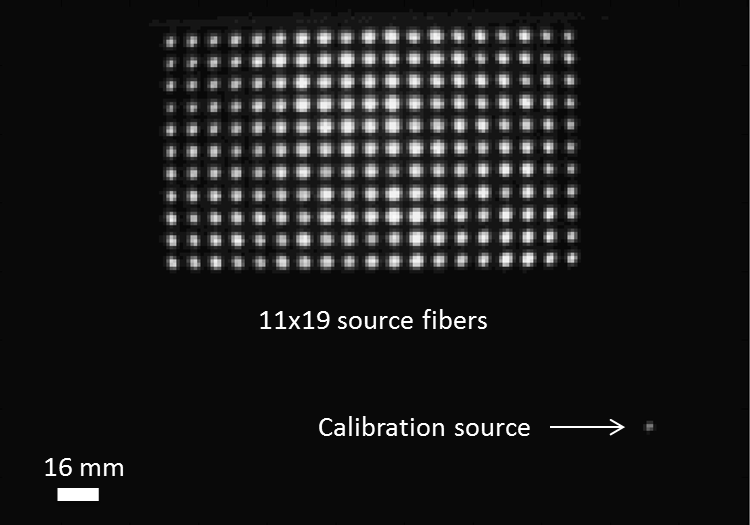
\includegraphics[width=10.5cm]{./figures/4_Gen3/srcplatepic2.png}
\caption{Source plate picture taken by Breast Imager CCD after it has been moved up to the detection window. The fibers are backlit by illuminating the back of the fiber bundle. This picture is used to determine the source position for reconstructions.}
\label{fig:srcplatepic}
\end{center}
\end{figure}


\subsection{Breast Tank and Patient Bed}
The breast imaging system is built around a modified biopsy patient bed. The bed allows for more of the breast to be inserted into the tank for greater breast coverage. The breast tank is located right below the hole in the biopsy patient bed. The tank consists a tank with a rail mounted source plate made out of black delrin to maintain parallel compression between the source plate and window. On the opposite side is an acrylic window with anti-reflective coating. The space between the window and the detection setup is covered by a light box that prevents stray signal from reaching the image intensifier and CCD. The tank is also mounted on ball-bearing surface which allows the breast tank, light box, and detection system to rotate 90 degrees for either sagittal or axial compression of the breast.

%\begin{figure}[t]
%\centering\includegraphics[width=7cm]{./figures/BiopsyBedPic.png}
%\caption{\label{fig:BiopsyBedPic}
%  Photograph of the (a) galvo switch and the (b) input face of the fiber bundle
%\end{figure}

\subsection{Image Intensifier mounted CCD}
The detection system consists of a back-illuminated EMCCD (Andor iXon DV887, Ireland) with quantum efficiency optimized in the $500-700\,{\rm nm}$ range. One of the most attractive features of this CCD was its "frame transfer" function which allows for shutterless continous measurement which would be beneficial for our heterodyne measurement scheme in Sec. \ref{sec:heterodyne}. This CCD is mounted with a gain-modulated image intensifier (Lambert Instruments, II8MD GENIII, Netherlands) with a P43 Phosphor screen with a peak emission at $545\, {\rm nm}$. The lens element in front of the image intensifier is a Xenon $25\,{\rm mm}$ $f/0.95$ C-Mount Lens for 1-Inch CCD (Schneider Optics, Germany). The $512 \times 512$ pixel CCD is cropped to a field of view of the breast tank window with a $2 \times 2$ hardware binning for an image $155 \times 200$ pixels with a dpixel of $0.33\, {\rm mm/pixel}$ with a 16-bit depth. The gain on the image intensifier is modulated at  $70\,{\rm MHz} + 1 {\rm Hz}$

\subsection{Frequency-Domain Heterodyne detection}
\label{sec:heterodyne}
The primary goal of the DOT system is to measure the amplitude attenuation and phase shift of the input light as it transits through the breast tissue. There are two approaches to demodulate a high frequency RF signal to estimate $\delta A$ and $\delta phi$: homodyne and heterodyne. Homodyne systems have been developed for optical imaging \cite{Troy1996,Sevick-Muraca1997,Godavarty2003}, but here we describe the heterodyne approach.

Our system uses the well known optical heterodyne detection scheme [cite] where the input signal $\omega_{s}$ is nonlinearly mixed with a reference signal at the same frequency which is offset by a small cross correlation frequency $\omega_{cc}$ such that $\omega_{g}=\omega_{s}+\omega_{cc}$ and the resulting beat frequency at $\omega_{cc}$ is measured.  In our system, $\omega_{s}$ and  $\omega_{g}$ are produced by a pair of phase-locked frequency generators. The lasers in the devices are modulated at $\omega_{s}=70\,{\rm MHz}$ such that the light source intensity can be described as
\begin{equation}
I(t) = I_{0} + I_{\omega}\cos(\omega_s t+\phi_I)
\end{equation}
where  $I_{0}$ is the DC amplitude, $I_{\omega}$ the AC amplitude and $\phi_I$ is the phase offset of the laser. When the light passes through our breast tank diffusively through breast or intralipid solution the resulting transmitted light has the form
\begin{equation}
T(t) = I_{0}A_{DC}({\bf r}) + I_{\omega}A_{AC}\cos(\omega_s t +\phi_I+ \phi({\bf r}))
\end{equation}
where $A_0$, $A_{AC}$, and $\phi$ are the spatially varying DC, AC, and phase information that we are measuring from the surface of our diffusive breast or intralipid solution. On the detection side, we modulate the gain of the image intensifier at $\omega_{g}=70\,{\rm MHz} + 1 {\rm Hz}$ so that the image intensifier sensitivity is
\begin{equation}
G(t) = G_{0} +G_{\omega} \cos((\omega_s+\omega_{cc})t+\phi_G))
\end{equation}
\noindent
where $G_{0}$ is the DC amplitude, $G_{\omega}$ the AC amplitude and $\phi_G$ is the phase offset of the image intensifier gain. The signal that is detected by the CCD after the image intensifier is then
\begin{equation}
S = I(t) \times G(t) = (I_{0} + I_{\omega}\cos(\omega_s t+\phi_I))(G_{0} +G_{\omega}\cos((\omega_s+\omega_{cc})t+\phi_G)).
\label{4_signal}
\end{equation}
The CCD measures the light intensity out of the image intensifer at rate of $10\, {\rm frames/s}$ with frame transfer mode with an exposure time $\sim100\, {\rm ms}$ which in addition to the phosphor screen response time of the image intensifier of $\sim{\rm ms}$ acts as a low pass filter on the signal. Thus (Eqn \ref{4_signal}) simplifies to
\begin{equation}
\label{eqn:heterodyne}
S  = I_{0}G_{0}A_{DC}({\bf r}) + I_{\omega}G_{\omega}A_{AC}\cos(\omega_{cc}t+\phi_I-\phi_G+\phi({\bf r})).
\end{equation}
where we are able to measure $I_{0}G_{0}A_{DC},\,I_{\omega}G_{\omega}A_{AC}$ and $\phi_I-\phi_G+\phi$ for each CCD pixel.

\subsection{DOT measurement and timing}
The measurement timing is controlled using a National Instruments DAQ board (serial) which has an onboard clock as well as analog and digital I/O which can be programmed via Labview software on a computer. The DAQ board is programmed to put out two syncronized clocked TTL signals at $10\,{\rm MHz}$ and $0.5\,{\rm Hz}$. The $10\,{\rm MHz}$ goes to the reference input of the two frequency generators to phase lock the two together. The 0.5Hz signal is sent to the CCD to trigger the beginning of the 17 sequential measurement series synchronizing to the heterodyne measurement via the frequency generators.

In our measurement protocol we switch through all the source positions for each wavelength in series. The measurement at each source position is two seconds long (each triggered by the $0.5\,{\rm Hz}$ signal) resulting in a total measurement time per scan of $2\,{\rm s} \times 209\,{\rm sources} \times 5$ wavelengths $\sim 35$ minutes. For each two second measurement, 17 exposures are captured at at $10\,{\rm frames/s}$ for a total of $1.7\,s$. The remaining $300 {\rm ms}$ is used to write data from the camera buffer to the computer harddrive and switch to the next source position and/or wavelength. To get the $I_{0}G_{0}A_{DC},\,I_{\omega}G_{\omega}A_{AC}$ and $\phi_I-\phi_G+\phi$ from the heterodyne measurement mentioned in Sec. \ref{sec:heterodyne}, the time series (over 17 frames) light intensity for each pixel is fit to Eqn. \ref{eqn:heterodyne} fitted for these variables as shown in Fig. \ref{fig:timeseries}. 
\begin{figure}[ht]
\begin{center}
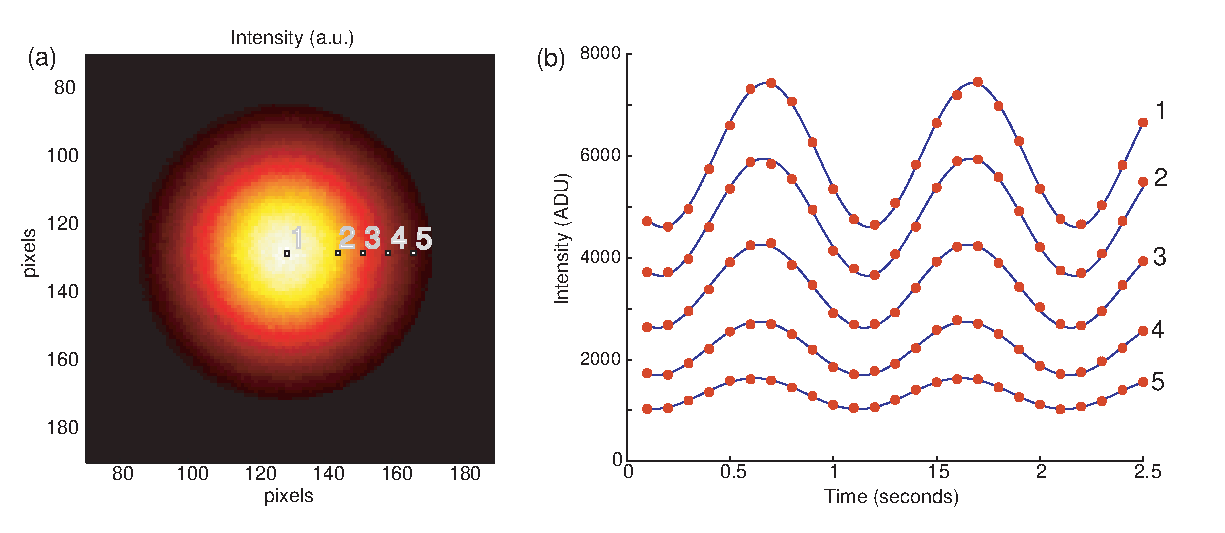
\includegraphics[width=14.5cm]{./figures/4_Gen3/timeseries.eps}
\caption{a) single time frame of light measured by the CCD. b) light intensities for pixels over time. This data is fit for DC, A, and $\phi$.}
\label{fig:timeseries}
\end{center}
\end{figure}

\section{Data Normalization}
\label{sec:datanorm}
A single breast scan will allow us to determine $I_{0}G_{0}A_{DC},\,I_{\omega}G_{\omega}A_{AC}$ and $\phi_I-\phi_G+\phi$ as we saw in Sec. \ref{sec:heterodyne}. However, the quantities that we are interested in are $A_{DC},\,A_{AC}$ and $\phi$ due to the optical properties of the breast. By taking a second reference scan with just the intralipid solution, we can divide out $I_{0}G_{0},\,I_{\omega}G_{\omega}$ and subtract out $\phi_I-\phi_G$.

In addition, we use a pickoff channel shown in Fig \ref{fig:gen3schem} to correct for any changes in amplitude or phase due to laser or RF instabilities before the galvo switch. 5 percent of the light is diverted using a 95/5 optical beam splitter and the fiber is run in front of the window with a 1-inch thick white delrin placed in front of the fiber tip used as a diffuser as shown in Fig \ref{fig:pickoffpic.jpg}. Because it is placed in the FOV of the window, this measurement is taken concurrently with each source measurement. An attenuator has been added to the pickoff so that the light level will be appropriate for the gain and dynamic range of the DOT measurement. 

Finally, we have one additional source of normalization that is used. The device has one additional source channel from the galvo switch which is placed very far from where the breast will be measured as shown in Fig \ref{fig:srcplatepic}. We call this the calibration source. Since it is just another source position fiber, this measurement is not taken concurrently, but rather in series with the DOT measurements. The calibration measurement is typically taken after every 10 sources. The advantage of this source is that is that unlike the pickoff, the calibration source corrects for the galvo and the reference tank and is useful for correcting long-term drifts in the system.

\section{Profilometry}
\label{sec:profilometry}
\subsection{Basics of Profilometry}
\begin{figure}[ht]
\begin{center}
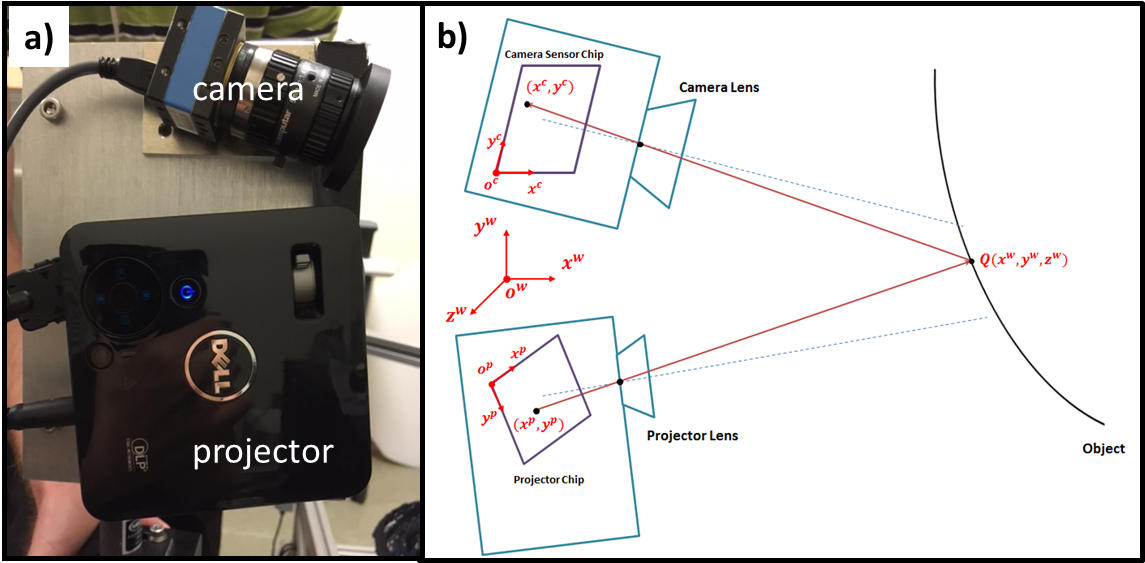
\includegraphics[width=14.5cm]{./figures/4_Gen3/profcoord.png}
\caption{a) Profilometry setup which consist of a ccd camera and a portable projector. b)the schematic with the coordinate systems for the camera, projector, and the world or object coordinate.}
\label{fig:profcoord}
\end{center}
\end{figure}
To improve our reconstruction quality, we have built two sets of imaging devices based on fringe projection profilometry technique. A review on various implementation of this technique can be found in \cite{}. We chose to implement the techniques proposed by Zhang et. al \cite{Zhang2006} with an emphasis on speed, reduced dependance on a need for projector gamma calibrations (which are time consuming). 
Fig. \ref{fig:profcoord} shows the picture of the profilometry device and the corresponding schematic with the related coordinate systems for the camera, projector, and the world or object coordinate. The basic principle of fringe projection profilometry is to project fringe patterns onto an object and to map the phase shift of the patterns to the object height. To accomplish this, one must calibrate the profilometry device to determine the spatial transform function between the camera, projector, and object coordinates. Then a calibration to determine the one-to-one function between the phase shift and object height. The calibration methods for this is detailed in the following references \cite{Peng2007,Zhang2010,Gorthi2010,Geng2011}.

Once the calibrations are set, obtaining the 3D surface profile of an object (in our case the breast surface) requires three steps: 1) projecting fringe patterns onto the object and measure the fringe distortions (Eqn. \ref{eqn:fringe}, 2) convert the distorted images into a phase map, and 3) unwrapping the phase as the phase map is limited to [$-\pi, \pi$].
\noindent
{\bf Step 1:} Project fringe patterns with the following equations:
\begin{eqnarray}
\label{eqn:fringe}
I_{c,1}(x_c,y_c) & = & I_{c,dc}(x_c,y_c)+I_{c,ac}(x_c,y_c)\cos(\phi_c(x_c,y_c)-2\pi/3)\nonumber \\
I_{c,2}(x_c,y_c) & = & I_{c,dc}(x_c,y_c)+I_{c,ac}(x_c,y_c)\cos(\phi_c(x_c,y_c))\nonumber\\
I_{c,3}(x_c,y_c) & = & I_{c,dc}(x_c,y_c)+I_{c,ac}(x_c,y_c)\cos(\phi_c(x_c,y_c)+2\pi/3)
\end{eqnarray}
\noindent
where $I_{c,dc}$ is the average intensity, $I_{c,dc}$ is the modulation amplitude and $\phi_c$ is the phase value to be solved to extract our high information. The subscript $c$ denotes that this is in the camera reference.
\noindent
{\bf Step 2:} convert into phase map by solving for $\phi_c$ using Eqn. \ref{eqn:fringe} which gives us
\begin{equation}
\phi_c(x_c,y_c)=\arctan\big(\frac{\sqrt{3}(I_{c,1}(x_c,y_c)-I_{c,3}(x_c,y_c)}{2I_{c,2}(x_c,y_c)-I_{c,3}(x_c,y_c)}\big).
\end{equation}
\noindent
{\bf Step 3:} Unwrap $\phi_c$ to get the unwrapped phase
\begin{equation}
\Phi_c(x_c,y_c)= \phi_c(x_c,y_c)+2\pi\cdot k(x_c,y_c)
\end{equation}
where $k$ is found by projecting an additional set of images on the object to encode binary information in the image as proposed by Zhang et. al \cite{Zhang2006}. The schematic diagram of the projections used and the binary encoding method is shown in Fig \ref{fig:profunwrap}. Implementing these steps, we are able to unwrap the phase in the steps are shown in Fig \ref{fig:proffringe}.
\begin{figure}[ht]
\begin{center}
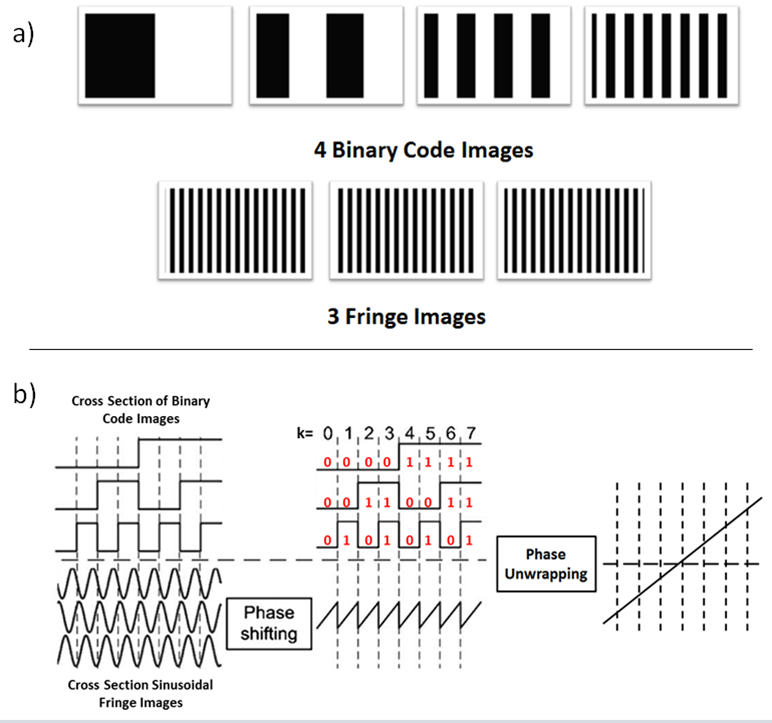
\includegraphics[width=14cm]{./figures/4_Gen3/profunwrap.png}
\caption{a) binary and fringe projections from the projector. b) unwrapping scheme proposed by Zhang et al. using the binary information encoded by the binary projections.}
\label{fig:profunwrap}
\end{center}
\end{figure}
\begin{figure}[ht]
\begin{center}
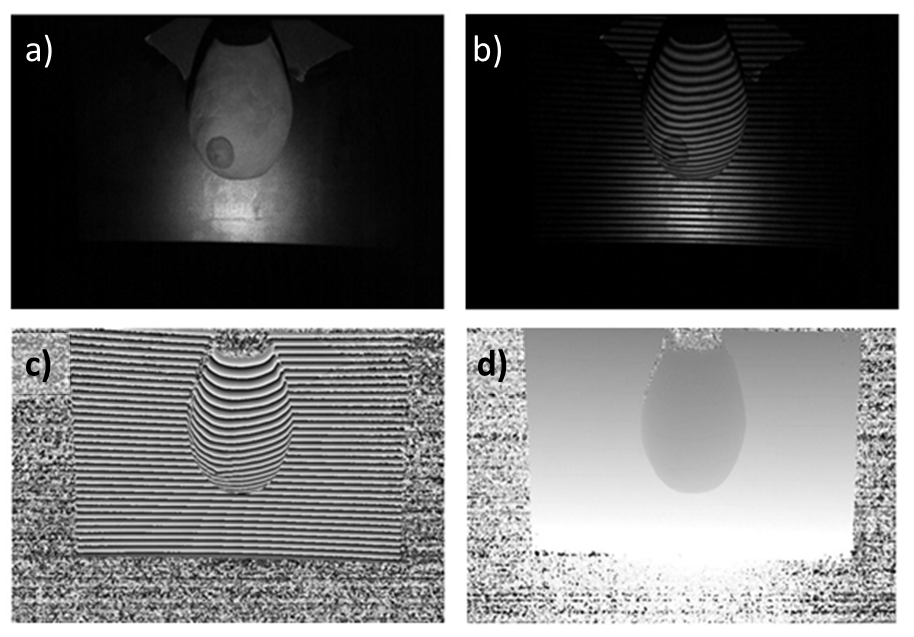
\includegraphics[width=14cm]{./figures/4_Gen3/proffringe.png}
\caption{a) object image b) fringe patterns projected onto object c) phase image d) unwrapped phase image.}
\label{fig:proffringe}
\end{center}
\end{figure}

\subsection{Profilometry for DOT segmentation}
The pair of profilometry devices we built are mounted on the DOT breast imager as show in Fig \ref{fig:proftank}. Fig \ref{fig:profdata} shows data from a human subject. Fringe pattern data is collected from each of the two profilometry devices as well as a sagittal image from the CCD where the outer edge has been traced by hand with a red line. The two surface point cloud generated by the profilometry phase map is combined with the outer trace (red line) of the breast image from the CCD to generate a 3D surface fit to generate a surface on the bottom side of the breast that was not illuminated by the profilometry projectors. This 3D surface fit is then used to generate a tetrahedral mesh to be used in the DOT image reconstruction.

\begin{figure}[ht]
\begin{center}
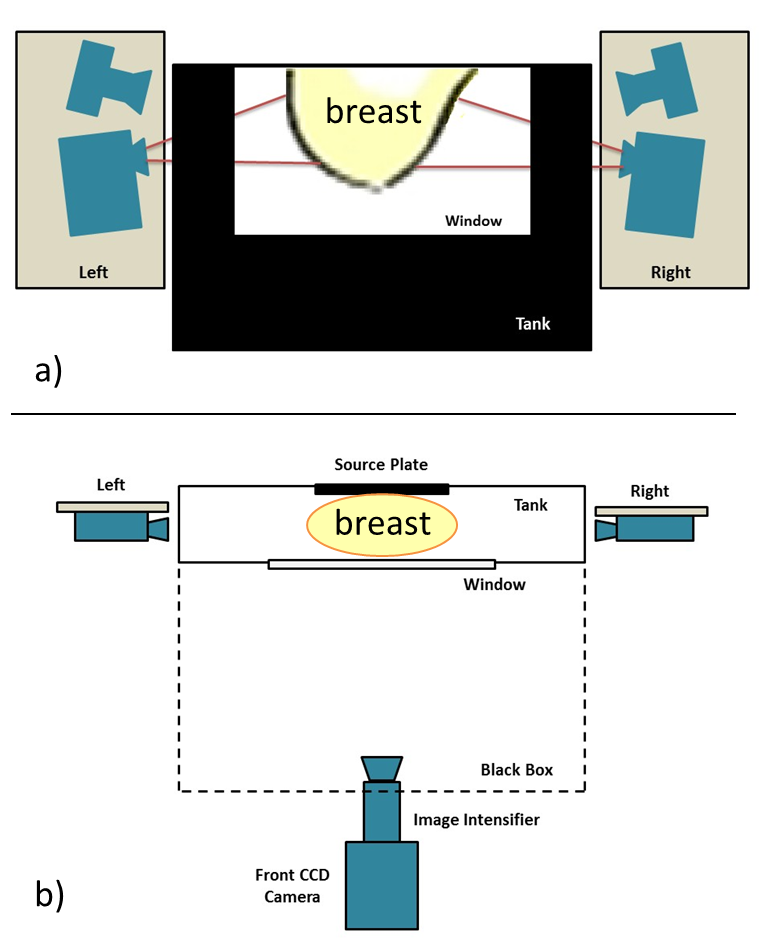
\includegraphics[width=12cm]{./figures/4_Gen3/proftank.png}
\caption{a) Front view of profilometry system with respect to Gen3 breast tank from perspective front CCD camera b) top view}
\label{fig:proftank}
\end{center}
\end{figure}
\begin{figure}[ht]
\begin{center}
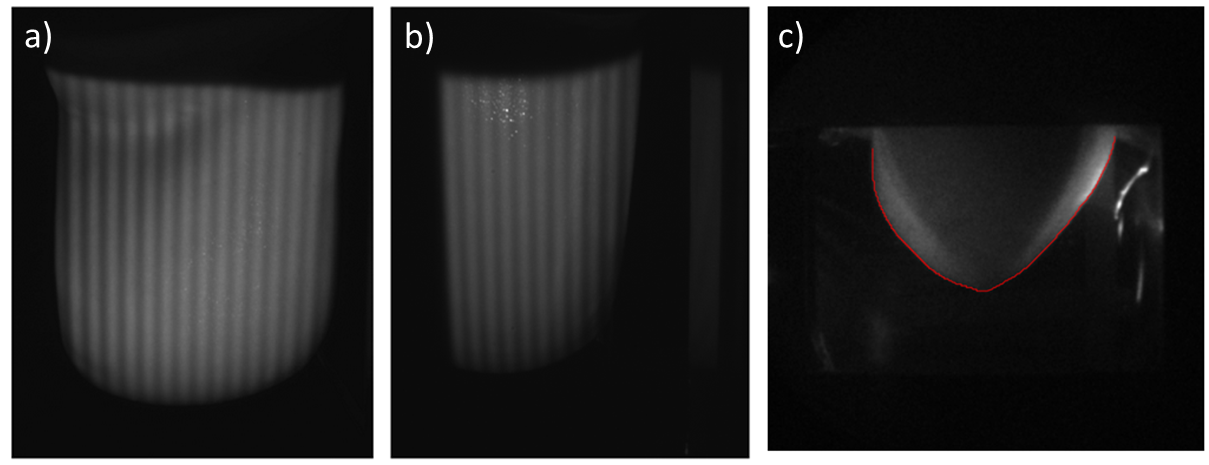
\includegraphics[width=12cm]{./figures/4_Gen3/profdata.png}
\caption{ a) fringe pattern projected on the breast (left side of tank) b) fringe pattern on right side of tank c) sagittal view of breast from front CCD. Red line shows outer edge of breast traced by hand.}
\label{fig:profdata}
\end{center}
\end{figure}
\begin{figure}[ht]
\begin{center}
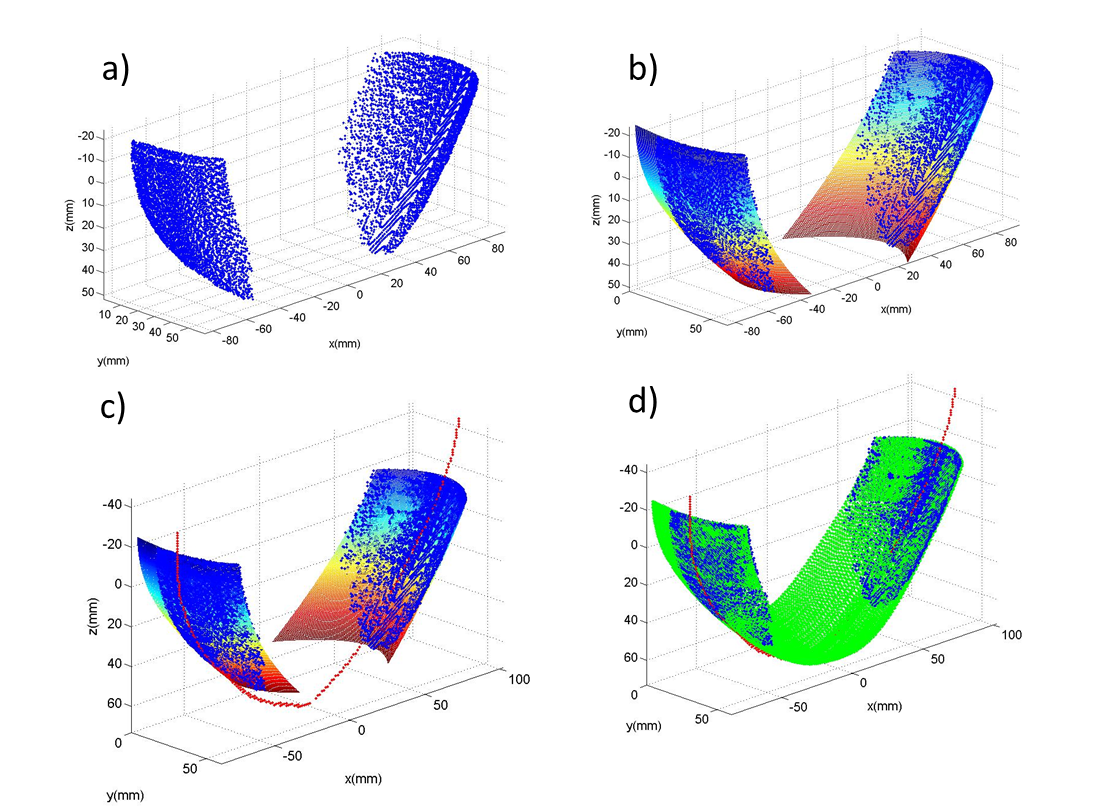
\includegraphics[width=14.5cm]{./figures/4_Gen3/proffit.png}
\caption{ a) 3D point cloud generated by fringe profilometry b)  surface fit of 3D point cloud c) line trace (red) from front CCD camera scaled and translated to match side surfaces d) 3D surface fit of whole breast generated from fringe profilometry data and front image trace.}
\label{fig:proffit}
\end{center}
\end{figure}

\section{Device characterization and testing}

\section{Clinical Results}
\chapter{Summary and Conclusion}

\section{Summary of main results}

\section{Limitations}

\section{Future Directions}
\appendix{Gen3 Software}
%\subappendix{Clinical Software}
\begin{figure}[h]
\centering
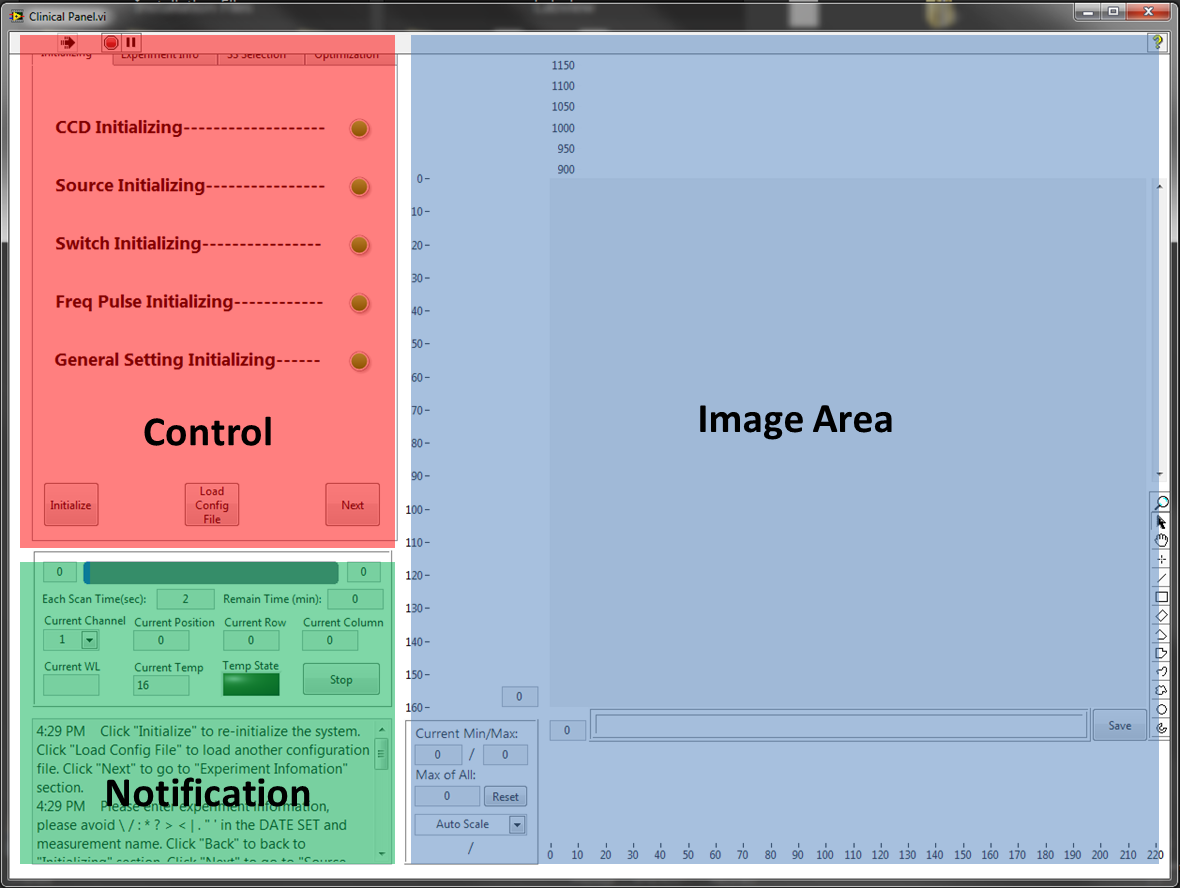
\includegraphics[width=13.5cm]{./figures/A_Gen3Software/Clinical1.png}
\caption[The Gen3 Clinical software written in Labview]{The Gen3 Clinical software written in Labview. The software consist of a control area (red) where the user interacts with the software, the notification area (area) where the instrument status and notifications are displayed, and the imaging area (blue) where the image from the Gen3 CCD is displayed.}
\label{fig:Clinical1}
\end{figure}
The Gen3 Clinical software was written with our clinical collaborators in mind. It minimizes access to the hardware and simplifies the measurement process to reduce user error. Figure~\ref{fig:Clinical1} shows the general layout of the software. The upper left area has the polymorphic interface controls (indicated in red) where the user mainly interacts with the software. Right below is the notification area (indicated in green) which displays the status of the instrument and various errors and notifications. Finally on the right is the image display (indicated in blue) where images from the Gen3 CCD is displayed.

The first panel that displays (Figure~\ref{fig:Clinical2}) is the initialization screen. Pressing the initialization button will do a system check of the CCD and the DAQ module.
\vspace{2mm}
\begin{figure}[bh]
\centering
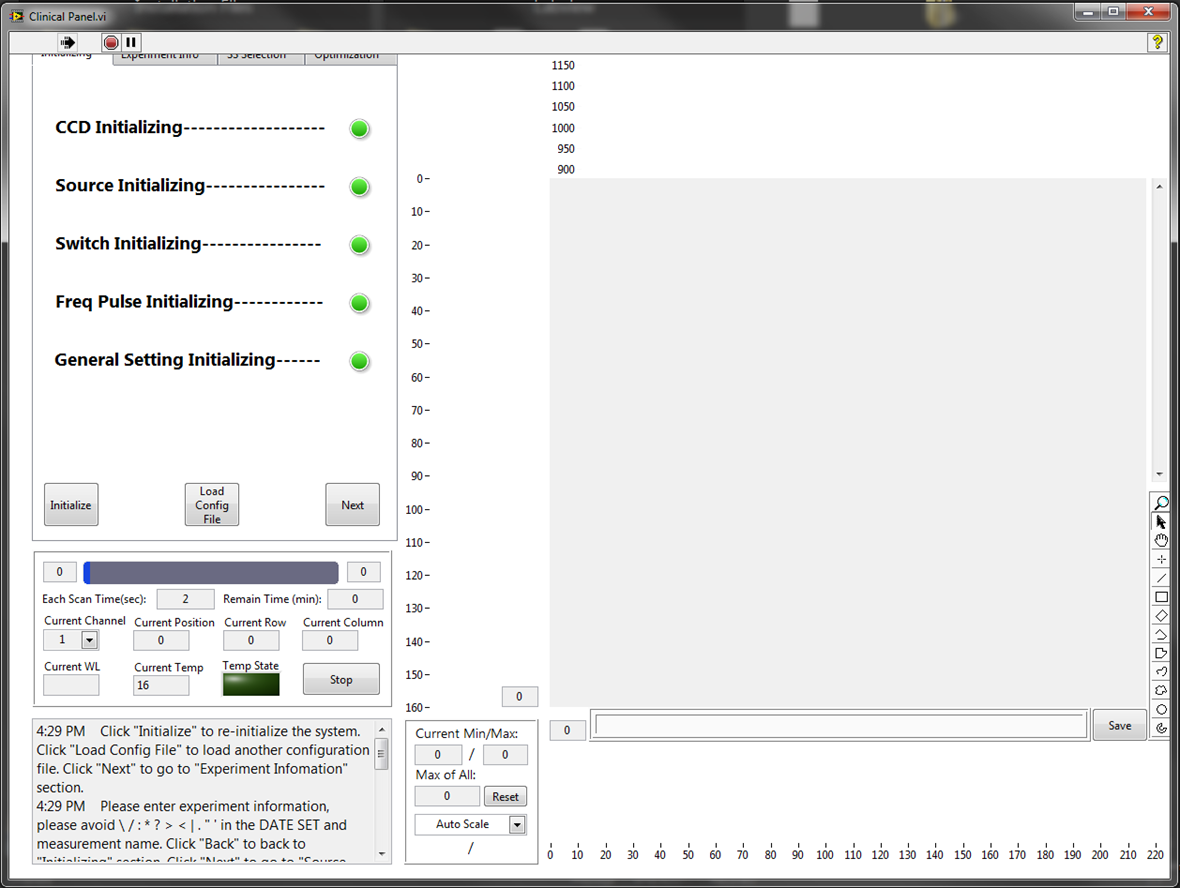
\includegraphics[width=13.5cm]{./figures/A_Gen3Software/Clinical2.png}
\caption[Initialization panel in the clinical software]{The first screen in the software is the initialization configuration screen. At this step, the hardware connection and statuses are checked before allowing the user to proceed. After the hardware status is checked, the user can load a preconfigured config file or proceed without one. The user can then continue onto the next step.}
\label{fig:Clinical2}
\end{figure}
If there are any errors or if these parts are disconnected, it will be indicated in the notification area. If all checks are successful and all green indicators are lit, the user can then load a configuration file (that has already been created in the Gen3 Experimental Software). Once a configuration file is loaded successfully, the user may proceed by clicking ``next". 

The proceeding screen is the Data input screen where the measurement details are recorded. The current date is automatically loaded and the control panel asks the user for the experiment number and the number of measurements. The minimum number of measurements is two: 1) one for the reference, and 2) one for a single breast measurement. The user can set up to 12 independent measurements before clicking ``next".
\begin{figure}[h]
\centering
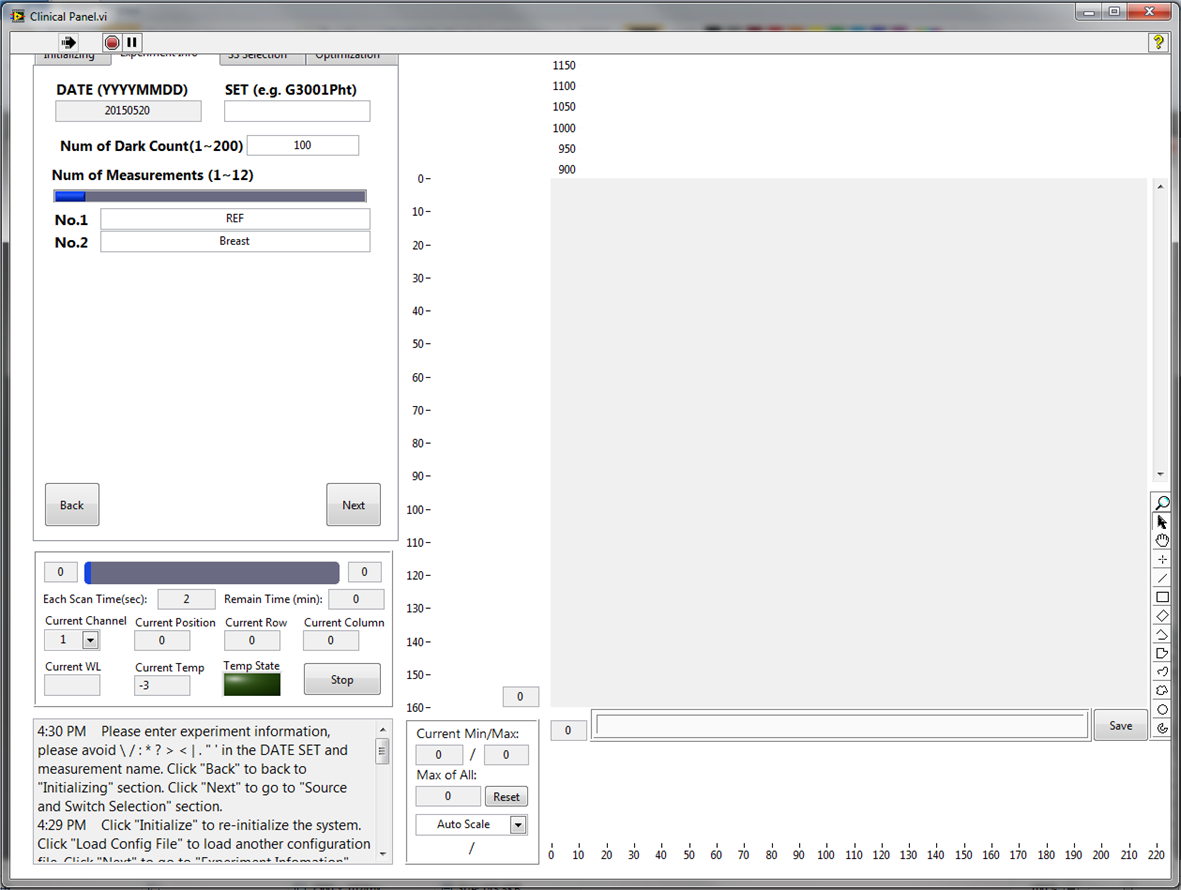
\includegraphics[width=13.5cm]{./figures/A_Gen3Software/Clinical3.png}
\caption[Measurement record panel in the clinical software]{The second panel is the Data input screen where the details of the measurement is entered. The patient number and the number of measurements can be indicated. The minimum number of measurements is two (typically for reference and a single breast measurement) but can be increased to 12.}
\label{fig:Clinical3}
\end{figure}

The third panel (Figure~\ref{fig:Clinical4}) in the clinical software is the source configuration screen. Here the user can choose the sources and wavelengths that will be used for the measurement. The first $11\times19$ indicators are for the source position. The second $11\times19$ grid is the calibration source grid. The user can indicate after which source the calibration measurement is taken. In Figure~\ref{fig:Clinical4}, for example, the calibration source is set to be taken after every 10th source. The sources sequence during the measurement moves from top left to the bottom right (this is hard coded). The last pair of $1\times 5$ indicator allow the user to choose the wavelengths for the sources and calibration sources respectively.

The fourth panel of the software shown in Figure~\ref{fig:Clinical5} the optimization panel. This panel is the first panel where the CCD and lasers can be controlled by the user. 
\begin{figure}[h]
\centering
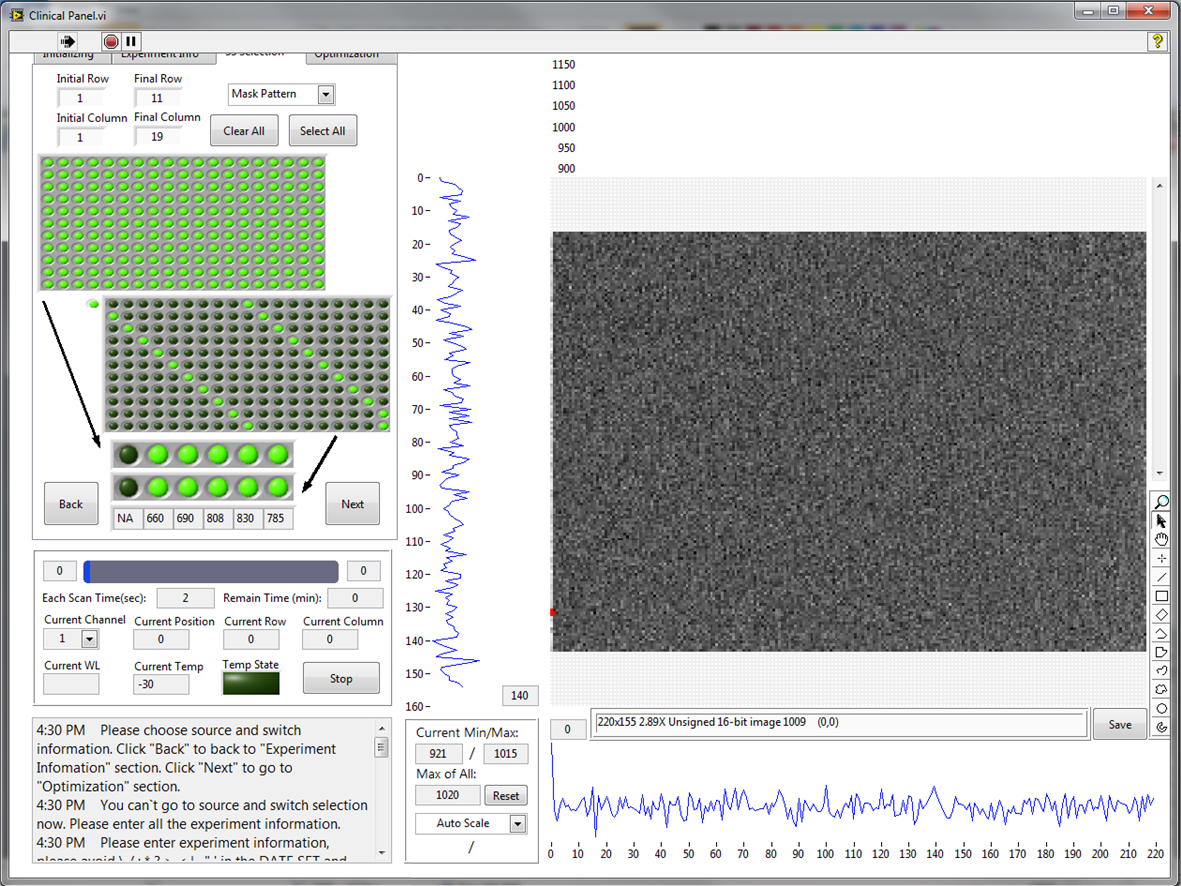
\includegraphics[width=13.5cm]{./figures/A_Gen3Software/Clinical4.png}
\caption[Measurement setup panel in the clinical software]{The third control panel is the source configuration screen. Here the source positions, the calibration measurements, and wavelengths used in the experiment can be chosen.}
\label{fig:Clinical4}
\end{figure}
At this panel, the detection gain and the laser intensities are adjusted so that the CCD not saturated for the particular breast or sourceplate detection window separation distance. The pickoff light level is adjusted at this stage. Note that the pickoff does not go through the imaging tank, so it must be adjusted independently of the laser sources.

The last panel in the clinical software is the measurement panel. At this point, the user can begin the measurements. The steps displayed on this screen is dependent on the entries in the previous panels. The user simply takes the measurement from the top to the bottom. The green light after each measurement description lights up indicating that the measurement is completed.
\vspace{3mm}
\begin{figure}[h]
\centering
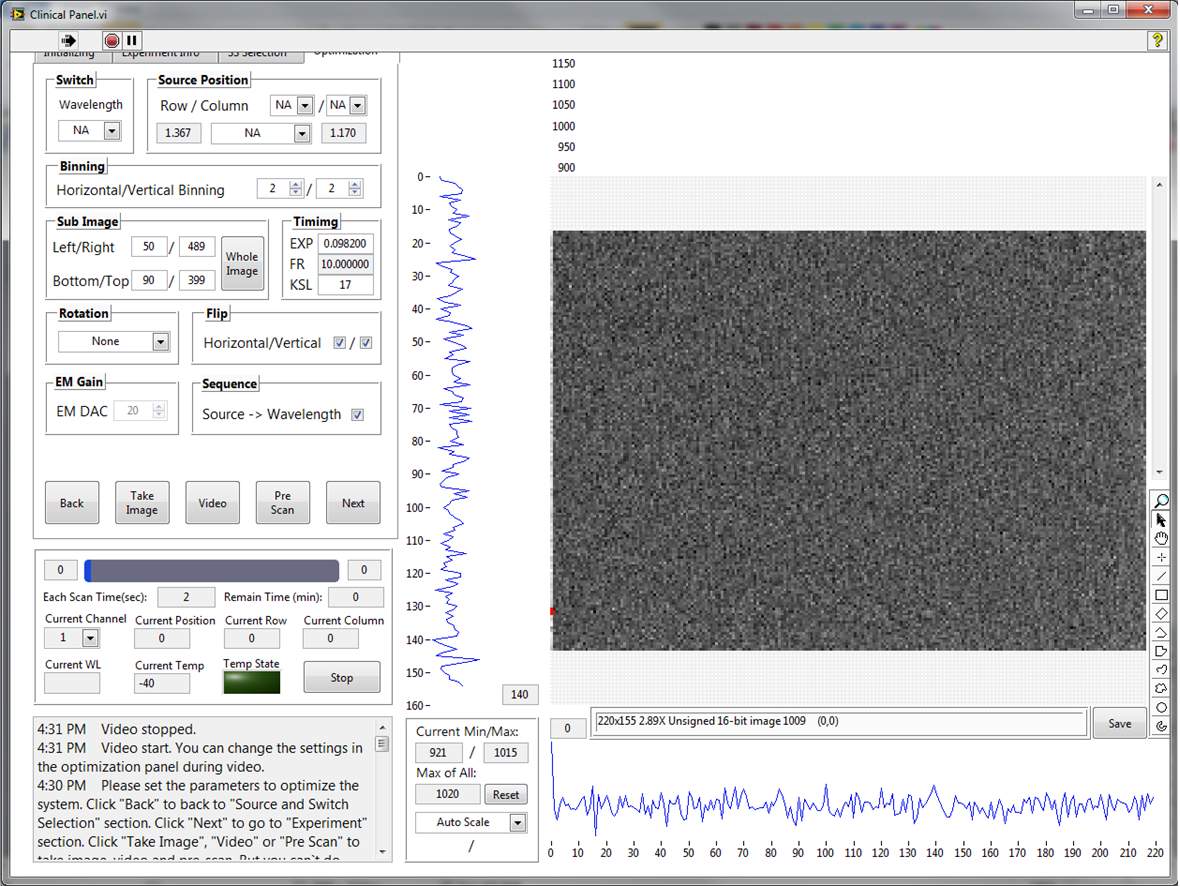
\includegraphics[width=13.5cm]{./figures/A_Gen3Software/Clinical5.png}
\caption[The optimization panel in the clinical software]{The measurement optimization screen. At this stage, the CCD can be run in video mode with the same exposure used in the actual measurements. The laser light level and detection gain is adjusted so that the CCD is not saturated or so that the light level is adequate for the current experiment.}
\label{fig:Clinical5}
\end{figure}
\begin{figure}[t]
\centering
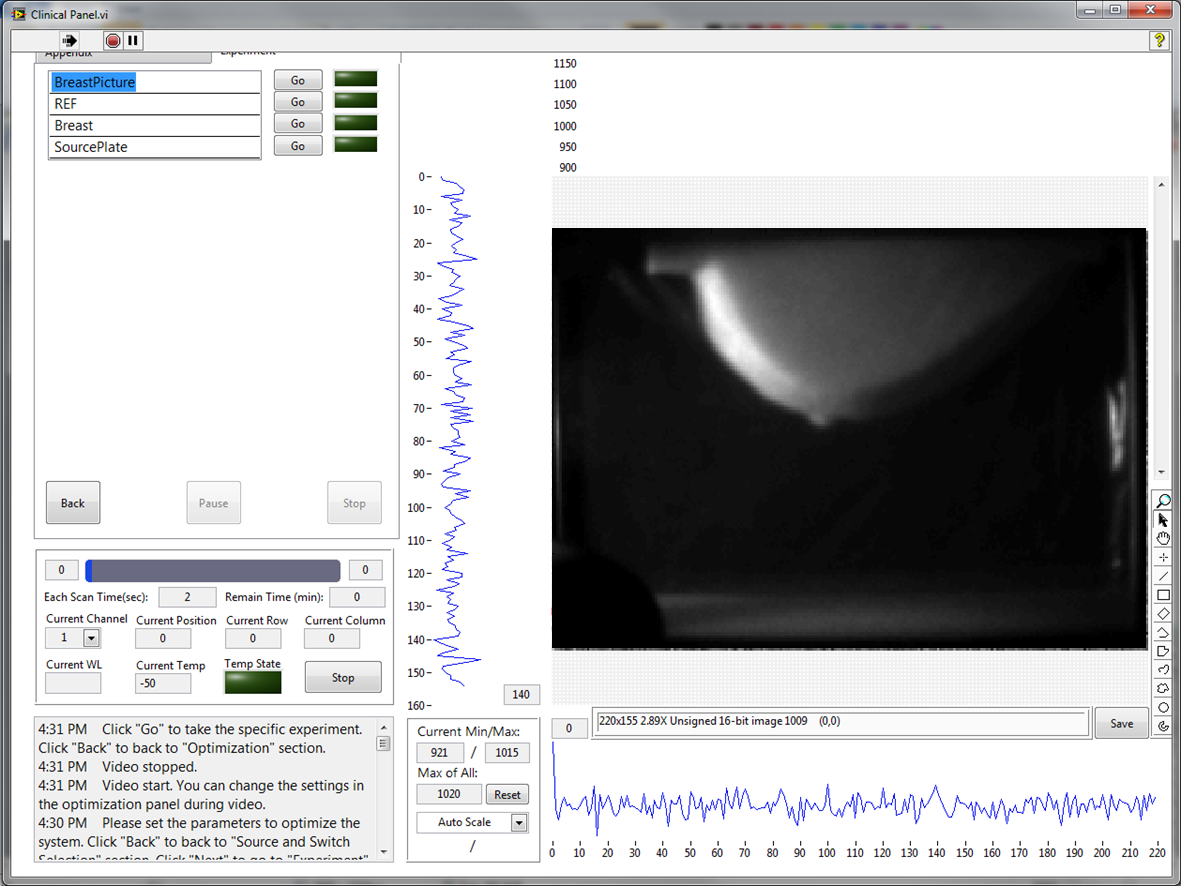
\includegraphics[width=13.5cm]{./figures/A_Gen3Software/Clinical6.png}
\caption[The measurement panel in the clinical software]{The measurement screen of the Gen3 clinical software. After setting up the experiment, the user takes the measurements in series on this screen by pressing the measurement buttons in sequence from top to bottom.}
\label{fig:Clinical6}
\end{figure}



\printgloss{../../../bibtexdatabase/glossarymastercopy}

\addcontentsline{toc}{chapter}{Bibliography}
\bibliographystyle{unsrt}
\bibliographystyle{plain}
\bibliography{Thesis}

\end{document}
